%%
%% Copyright (c) 2019 Weitian LI <liweitianux@sjtu.edu.cn>
%% Creative Commons BY 4.0
%%

\documentclass{beamer}

%%
%% Copyright (c) 2019 Weitian LI <liweitianux@sjtu.edu.cn>
%% Creative Commons BY 4.0
%%

\usetheme{metropolis}
\metroset{progressbar=foot}

\setbeamertemplate{section in toc}[sections numbered]
% Numbered sections in section page
% Credit: https://github.com/matze/mtheme/issues/271#issuecomment-292799444
\makeatletter
\setbeamertemplate{section page}{
  \centering
  \begin{minipage}{25em}
    \raggedright
    \usebeamercolor[fg]{section title}
    \usebeamerfont{section title}
    \thesection.~\insertsectionhead\\[-1ex]
    \usebeamertemplate*{progress bar in section page}
    \par
    \ifx\insertsubsectionhead\@empty\else%
      \usebeamercolor[fg]{subsection title}%
      \usebeamerfont{subsection title}%
      \thesection.\thesubsection.~\insertsubsectionhead
    \fi
  \end{minipage}
  \par
  \vspace{\baselineskip}
}
\makeatother

\setbeamertemplate{frametitle continuation}{(\insertcontinuationcount)}
\setbeamertemplate{bibliography item}{\insertbiblabel}

\setbeamertemplate{itemize items}[circle]
\setbeamertemplate{itemize subitem}[triangle]
% Suppress itemize indentation
% Credit: https://tex.stackexchange.com/a/450317
\settowidth{\leftmargini}{\usebeamertemplate{itemize item}}
\addtolength{\leftmargini}{\labelsep}
\settowidth{\leftmarginii}{\usebeamertemplate{itemize subitem}}
\addtolength{\leftmarginii}{\labelsep}

%\usepackage{pgfpages}
%\setbeameroption{hide notes}  % only slides
%\setbeameroption{show only notes}  % only notes
%\setbeameroption{show notes on second screen=right}  % both

% Solarized theme
% Credit: https://ethanschoonover.com/solarized/
\definecolor{SolBase02}{HTML}{073642}
\definecolor{SolBase3}{HTML}{fdf6e3}
\definecolor{SolOrange}{HTML}{cb4b16}
\definecolor{SolGreen}{HTML}{859900}
%
\setbeamercolor{normal text}{fg=SolBase02, bg=SolBase3}
%\setbeamercolor{normal text}{bg=white}  % for print
\setbeamercolor{alerted text}{fg=SolOrange}
\setbeamercolor{example text}{fg=SolGreen}

\setsansfont{Fira Sans Light}[
  BoldFont={Fira Sans Medium}
]
\setmonofont{Fira Code Light}[
  BoldFont={Fira Code Medium}
]

\usepackage{bm}
\usepackage{newtxsf}
\newcommand{\R}[1]{\text{#1}}  % text math alphabets
\newcommand{\Ce}{\R{e}}  % constant e
\newcommand{\Ci}{\R{i}}  % constant i
\newcommand{\Cpi}{\piup}  % upright 'pi', provided by 'newtxsf' package
\newcommand{\B}[1]{\bm{\mathsf{#1}}}  % single-letter bold math
\newcommand{\D}[1]{\R{d}#1}
\newcommand{\diff}[2]{\frac{\D{#1}}{\D{#2}}}
\newcommand{\pdiff}[2]{\frac{\partial #1}{\partial #2}}

\usepackage{xeCJK}
\setCJKsansfont{Source Han Sans SC Light}[
  BoldFont={Source Han Sans SC Medium}
]

\usepackage{hyperref}
\hypersetup{
  pdfstartview={Fit}
}

\usepackage{appendixnumberbeamer}
\usepackage{booktabs}
\usepackage{csquotes}

\usepackage{caption}
\captionsetup{%
  figurename={图},
  format=plain,
  labelformat=simple,
  labelsep=period,
  justification=centering,
  textfont={footnotesize},
  labelfont={footnotesize},
}

\usepackage{keyval}
\usepackage{etoolbox}

\makeatletter
% Set the keys (arguments) for including a figure
\newlength{\myfigure@width}
\newlength{\myfigure@height}
\newtoggle{myfigure@vertcap}
\define@key{myfigure}{width}{\setlength\myfigure@width{#1}}
\define@key{myfigure}{height}{\setlength\myfigure@height{#1}}
\define@key{myfigure}{vertcap}[true]{\toggletrue{myfigure@vertcap}}
%
% Custom command to include a figure with a horizontal/vertical caption
\NewDocumentCommand{\myfigure}{m m m}{
  \setkeys{myfigure}{width=0pt, height=0pt, #1}
  %
  % Get the size that a figure is being rendered
  % Credit: https://tex.stackexchange.com/a/3664
  \newsavebox{\myfigure@box}
  \ifdimequal{\myfigure@height}{0pt}{
    \savebox{\myfigure@box}{%
      \includegraphics[width=\myfigure@width]{#2}}
  }{%
    \savebox{\myfigure@box}{%
      \includegraphics[height=\myfigure@height]{#2}}
  }
  \settowidth{\myfigure@width}{\usebox{\myfigure@box}}
  \settoheight{\myfigure@height}{\usebox{\myfigure@box}}
  %
  \begin{figure}[!h]
    \centering
    \usebox{\myfigure@box}
    \iftoggle{myfigure@vertcap}{%
      \hspace{-0.5em}%
      % Credit: https://tex.stackexchange.com/a/44433
      \rotatebox{90}{%
        \begin{minipage}{\myfigure@height}
          \caption{#3}
        \end{minipage}
      }
    }{%
      \caption{#3}
    }
  \end{figure}
  % Credit: https://tex.stackexchange.com/a/18174
  \global\let\myfigure@box\relax
}
%
\makeatother

\usepackage{xparse}
% Credit: https://tex.stackexchange.com/a/376366
\ExplSyntaxOn
\NewDocumentCommand{\cspace}{O{1em}}{%
  \tl_map_inline:nn {空} { \makebox[#1]{\phantom{##1}} }
}
\ExplSyntaxOff

\usepackage{siunitx}
% siunitx settings and new units
\sisetup{
  range-phrase=\text{--},
  range-units=single,
  product-units=repeat,
  list-separator={, },
  list-final-separator={, and },
  separate-uncertainty=true,
  detect-all,  % detecting fonts
}
%
\DeclareSIUnit\arcsec{arcsec}
\DeclareSIUnit\arcmin{arcmin}
\DeclareSIUnit\cMpc{cMpc}  % comoving Mpc
\DeclareSIUnit\cGpc{cGpc}  % comoving Gpc
\DeclareSIUnit\deg{deg}
\DeclareSIUnit\dyne{dyn}
\DeclareSIUnit\erg{erg}
\DeclareSIUnit\esu{esu}
\DeclareSIUnit\franklin{Fr}
\DeclareSIUnit\gauss{G}
\DeclareSIUnit\hubble{\ensuremath{\mathit{h}}}
\DeclareSIUnit\jansky{Jy}
\DeclareSIUnit\lightyear{ly}
\DeclareSIUnit\parsec{pc}
\DeclareSIUnit\rayleigh{Rayleigh}
\DeclareSIUnit\solarmass{\ensuremath{\text{M}_{\odot}}}
\DeclareSIUnit\statcoulomb{statC}
\DeclareSIUnit\year{yr}
%
\DeclareSIUnit\kpc{\kilo\parsec}
\DeclareSIUnit\mJy{\milli\jansky}
\DeclareSIUnit\mK{\milli\kelvin}
\DeclareSIUnit\Gpc{\giga\parsec}
\DeclareSIUnit\Gyr{\giga\year}
\DeclareSIUnit\Mpc{\mega\parsec}
\DeclareSIUnit\Myr{\mega\year}
\DeclareSIUnit\uG{\micro\gauss}

\usepackage{journalabbrv}

\usepackage[%
  backend=biber,
  style=authoryear-comp,
]{biblatex}

\AtBeginBibliography{
  \linespread{1.0}
  \footnotesize
}
\addbibresource{../references.bib}

\graphicspath{
  {./}
  {figures/}
  {../figures/}
  {../figures/self/}
  {../sjtuthesis/}
}

% Change 'emph' style to bold face
\let\emph\relax  % there's no \RedeclareTextFontCommand
\DeclareTextFontCommand{\emph}{\boldmath\bfseries}

\newcommand{\email}[1]{\href{mailto:#1}{\texttt{#1}}}
\newcommand{\doi}[1]{\href{https://doi.org/#1}{\textsc{doi}:#1}}
\newcommand{\ads}[1]{\href{http://adsabs.harvard.edu/abs/#1}{\textsc{ads}:#1}}
\newcommand{\arxiv}[1]{\href{https://arixv.org/abs/#1}{\textsc{arXiv}:#1}}

\endinput



%=====================================================================

\subject{博士学位论文答辩}
\titlegraphic{%
  
\includegraphics[height=0.75cm]{sjtubadge}%
  \hspace{2mm}%
  
\includegraphics[height=0.75cm]{sjtulogo}%
}
\title{%
  SKA EoR 探测实验的射电晕前景建模以及\texorpdfstring{\\}{ }%
  EoR 信号分离算法的研究%
}
\author{%
  答辩人:李维天\texorpdfstring{\\}{ / }
  导师:徐海光~教授\texorpdfstring{\\}{ / }
  专业:物理学
}
\institute{%
  物理与天文学院\\%
  上海交通大学%
}
\date{\small 2019 年 9 月 6 日}


%=====================================================================

\begin{document}

\maketitle

\begin{frame}{提\cspace{}纲}
  \tableofcontents[hideallsubsections]
\end{frame}


%=====================================================================
\section{研究背景和内容}

%............
\begin{frame}{什么是 EoR ?}
  \begin{itemize}
    \item \alert{再电离时期 (EoR)}:大爆炸之后约 \numrange{3}{10} 亿年,
      红移约 \numrange{6}{15}
    \item \alert{重要意义}:第一代恒星和星系、宇宙早期结构形成、
      宇宙演化关键环节之一
    \item 亟待深入理解的一个重要时期
  \end{itemize}

  \vspace{-1ex}
  \begin{figure}
    \centering
    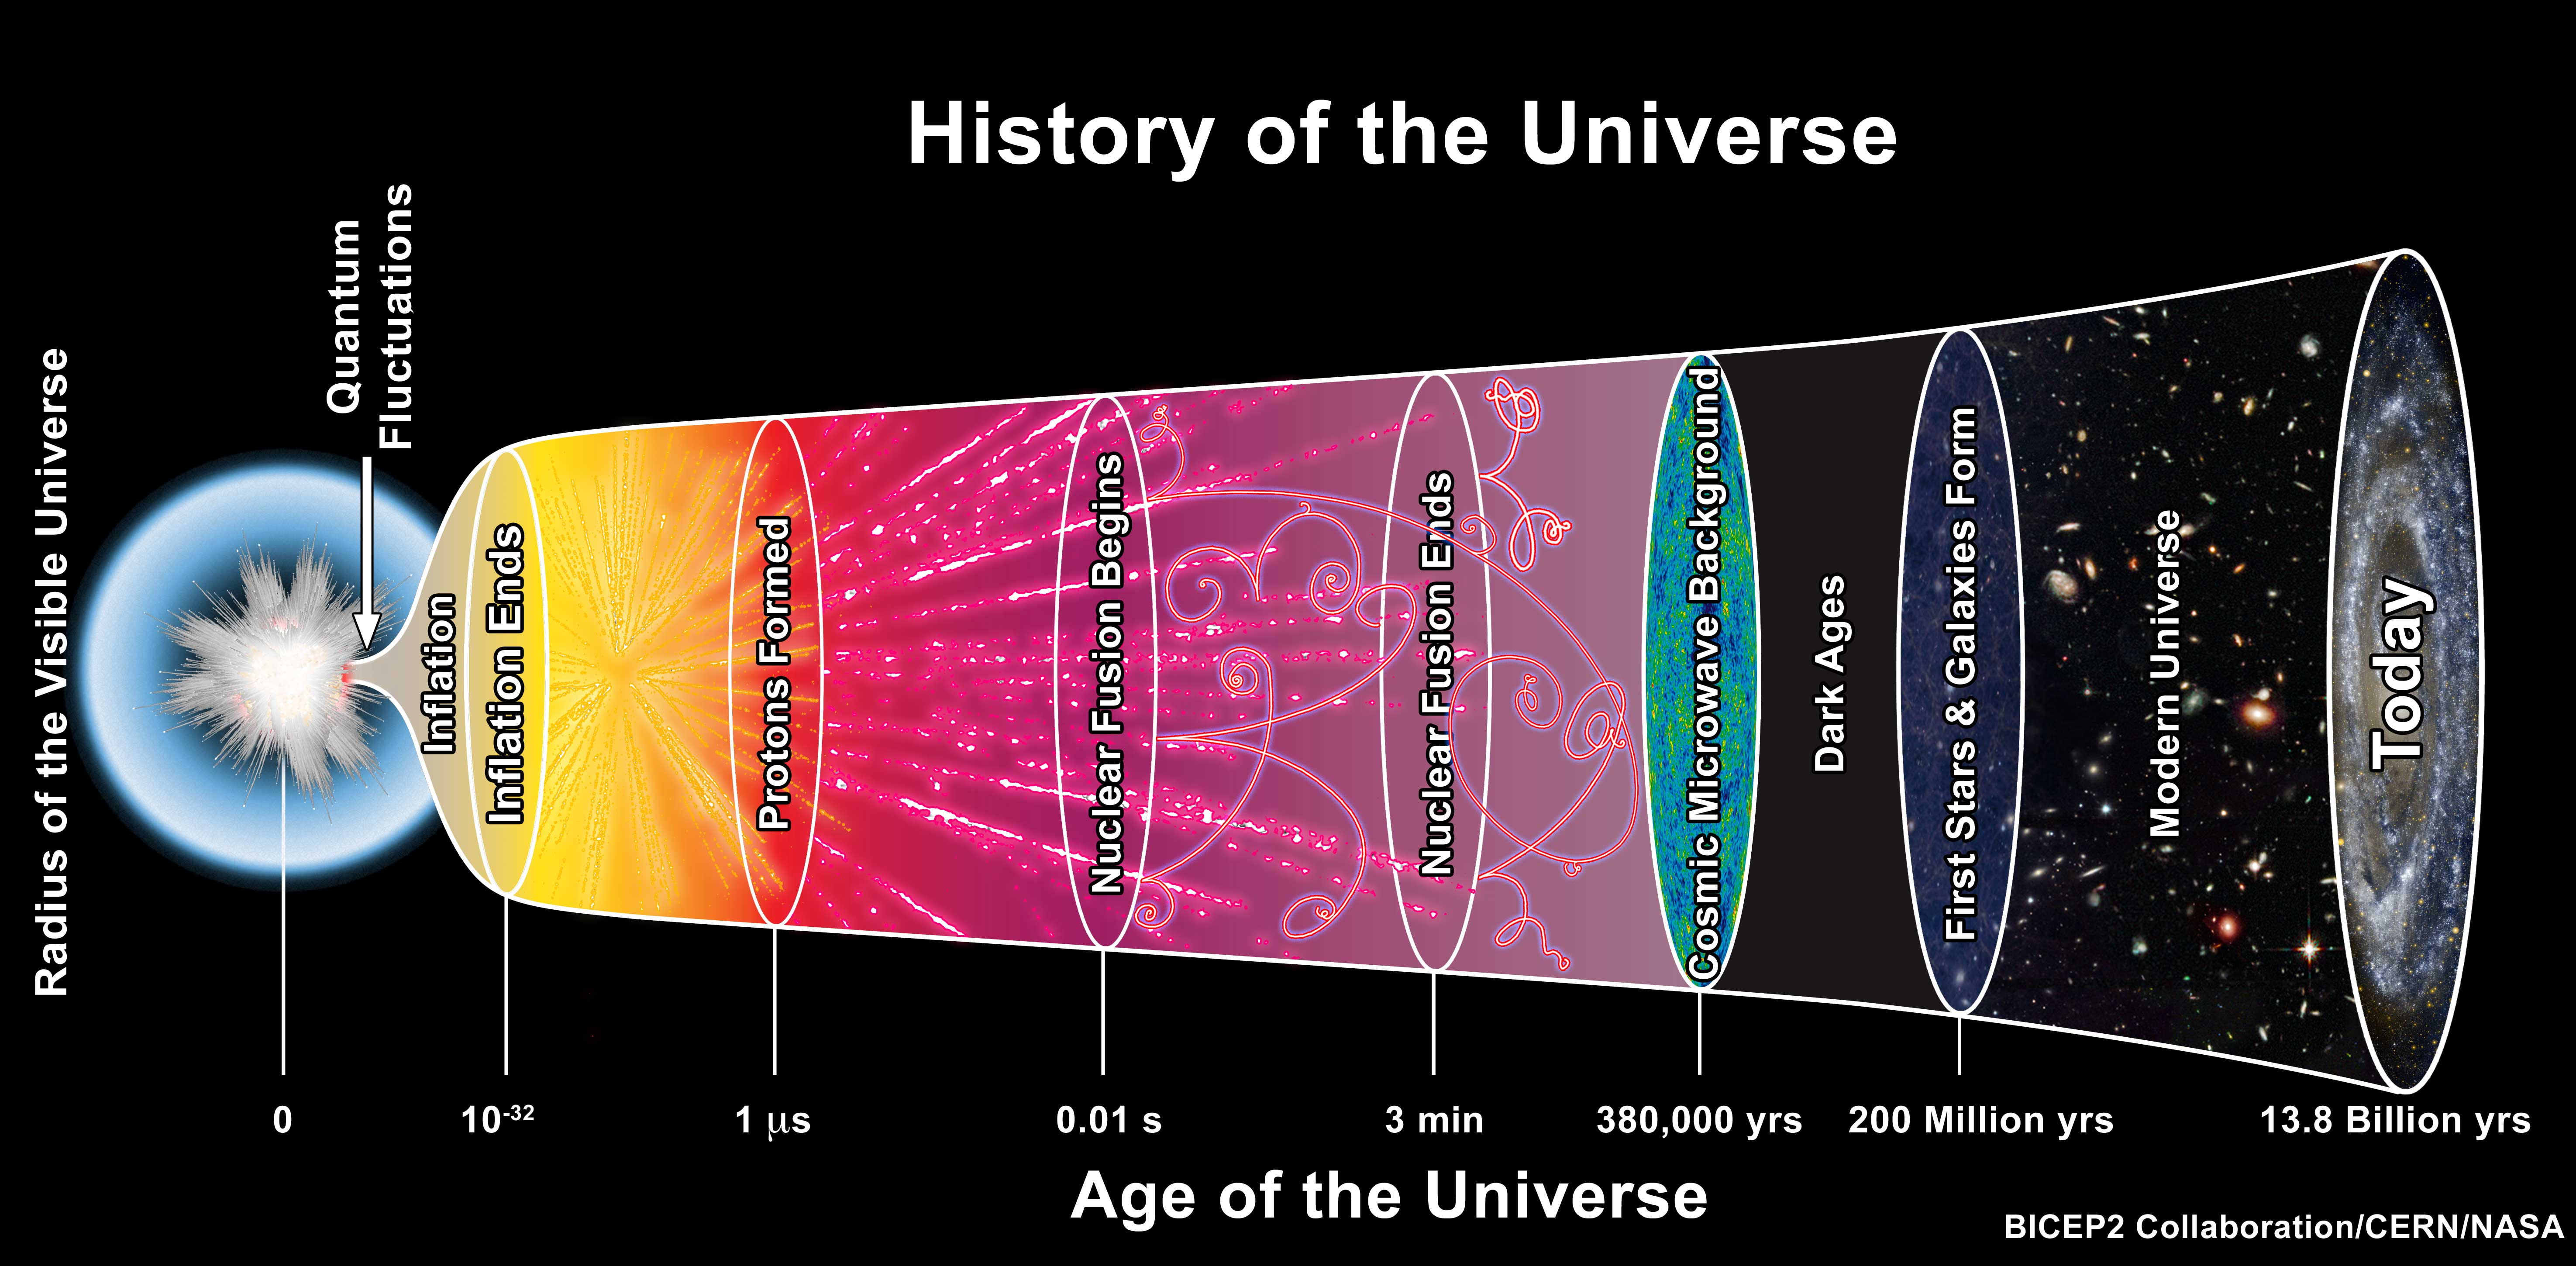
\includegraphics[width=0.95\textwidth]{universe-history}
  \end{figure}

  \blfootnote{图片来源: BICEP2/CERN/NASA (CC0)}
\end{frame}

%............
\begin{frame}{如何探测 EoR ?}
  \begin{columns}[onlytextwidth]
    \column{0.7\textwidth}
    \begin{itemize}
      \item \alert{中性氢 21\,cm 谱线}:EoR 最直接有效的探针
      \item 氢原子自旋翻转跃迁,本征频率 $\sim$\,\SI{1420}{\MHz}
      \item EoR 信号将出现在 $\sim$\,\SIrange{90}{200}{\MHz}
        的\alert{低频射电波段}
    \end{itemize}

    \column{0.3\textwidth}
    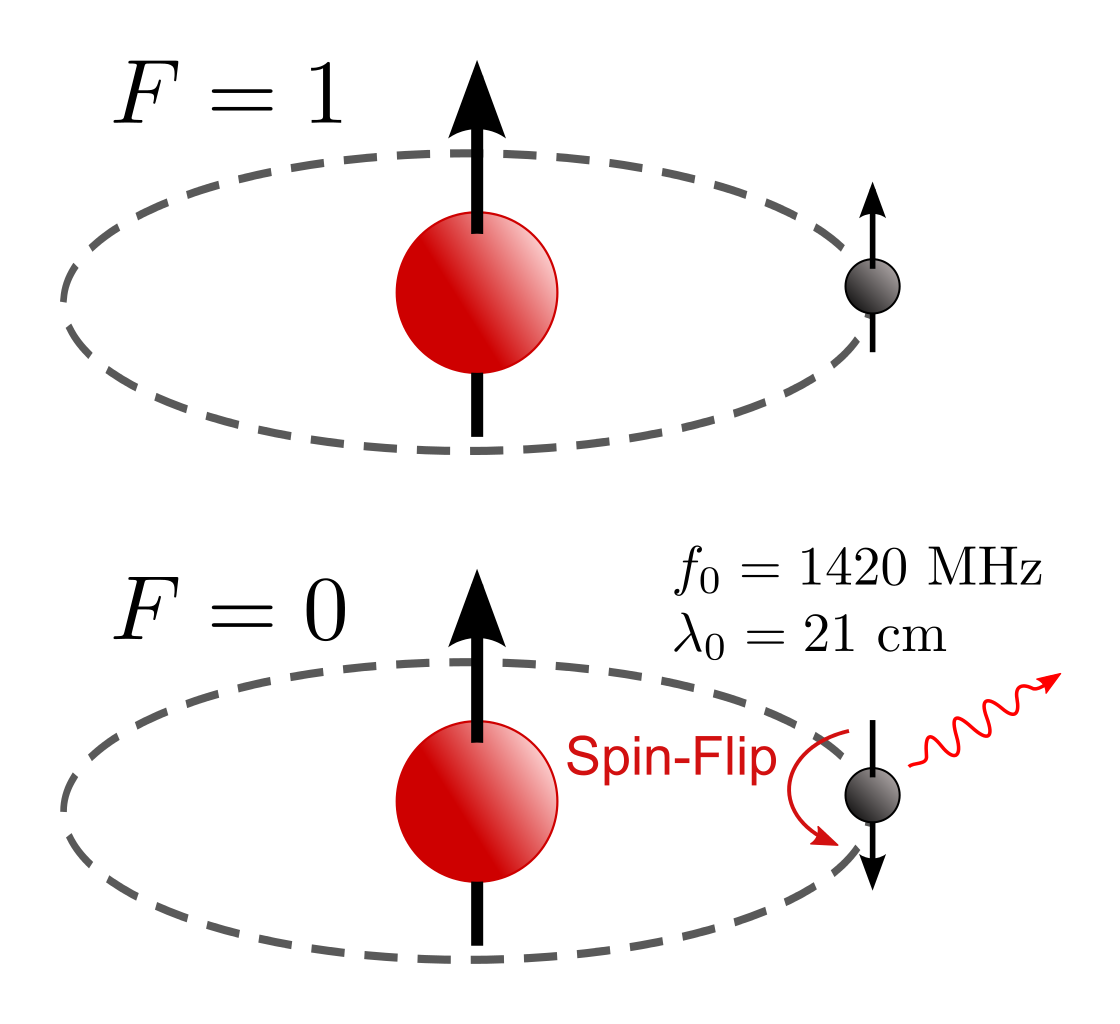
\includegraphics[width=\columnwidth]{hydrogen-spinflip}
  \end{columns}

  \vspace{-1ex}
  \begin{figure}
    \centering
    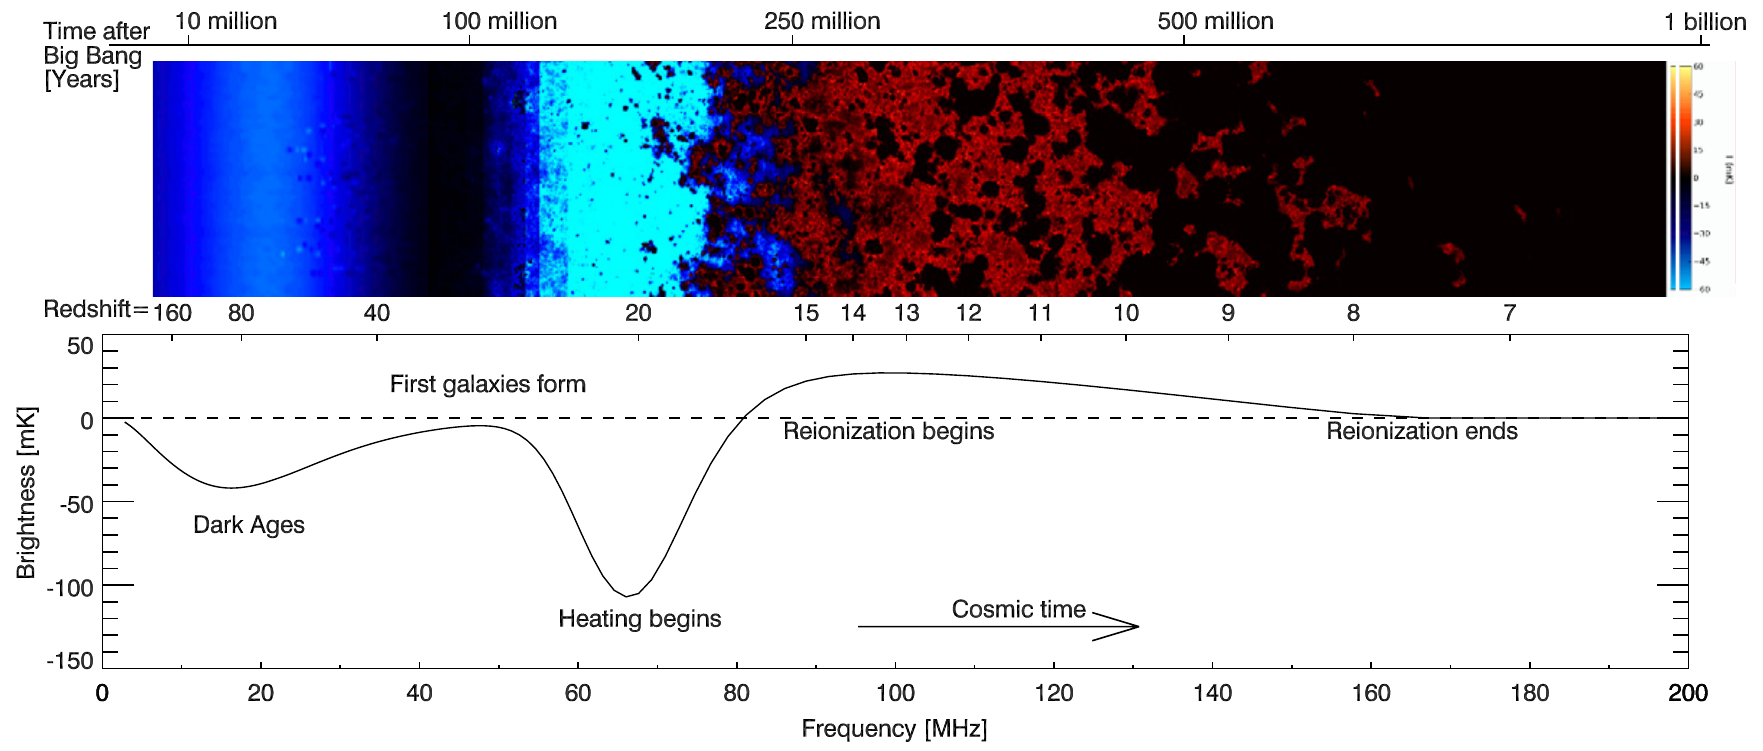
\includegraphics[width=0.95\textwidth]{eor-signal-evolution}
  \end{figure}
  \vspace{1ex}
  \blfootnote{图片来源: (1) Wikipedia; (2) \cite{pritchard2012}}
\end{frame}

%............
\begin{frame}{前景干扰:EoR 探测主要困难之一}
  \begin{itemize}
    \item EoR 信号非常微弱 ($\sim$\,\SI{10}{\mK} @ \SI{150}{\MHz})
    \item \alert{多种前景干扰},比待测信号强 $\sim$\,4--5 个数量级
    \item \alert{对策}:深入理解前景干扰,构建准确的前景模型,
      研发有效的前景处理和 EoR 信号分离算法
  \end{itemize}

  \vspace{-1ex}
  \begin{figure}
    \centering
    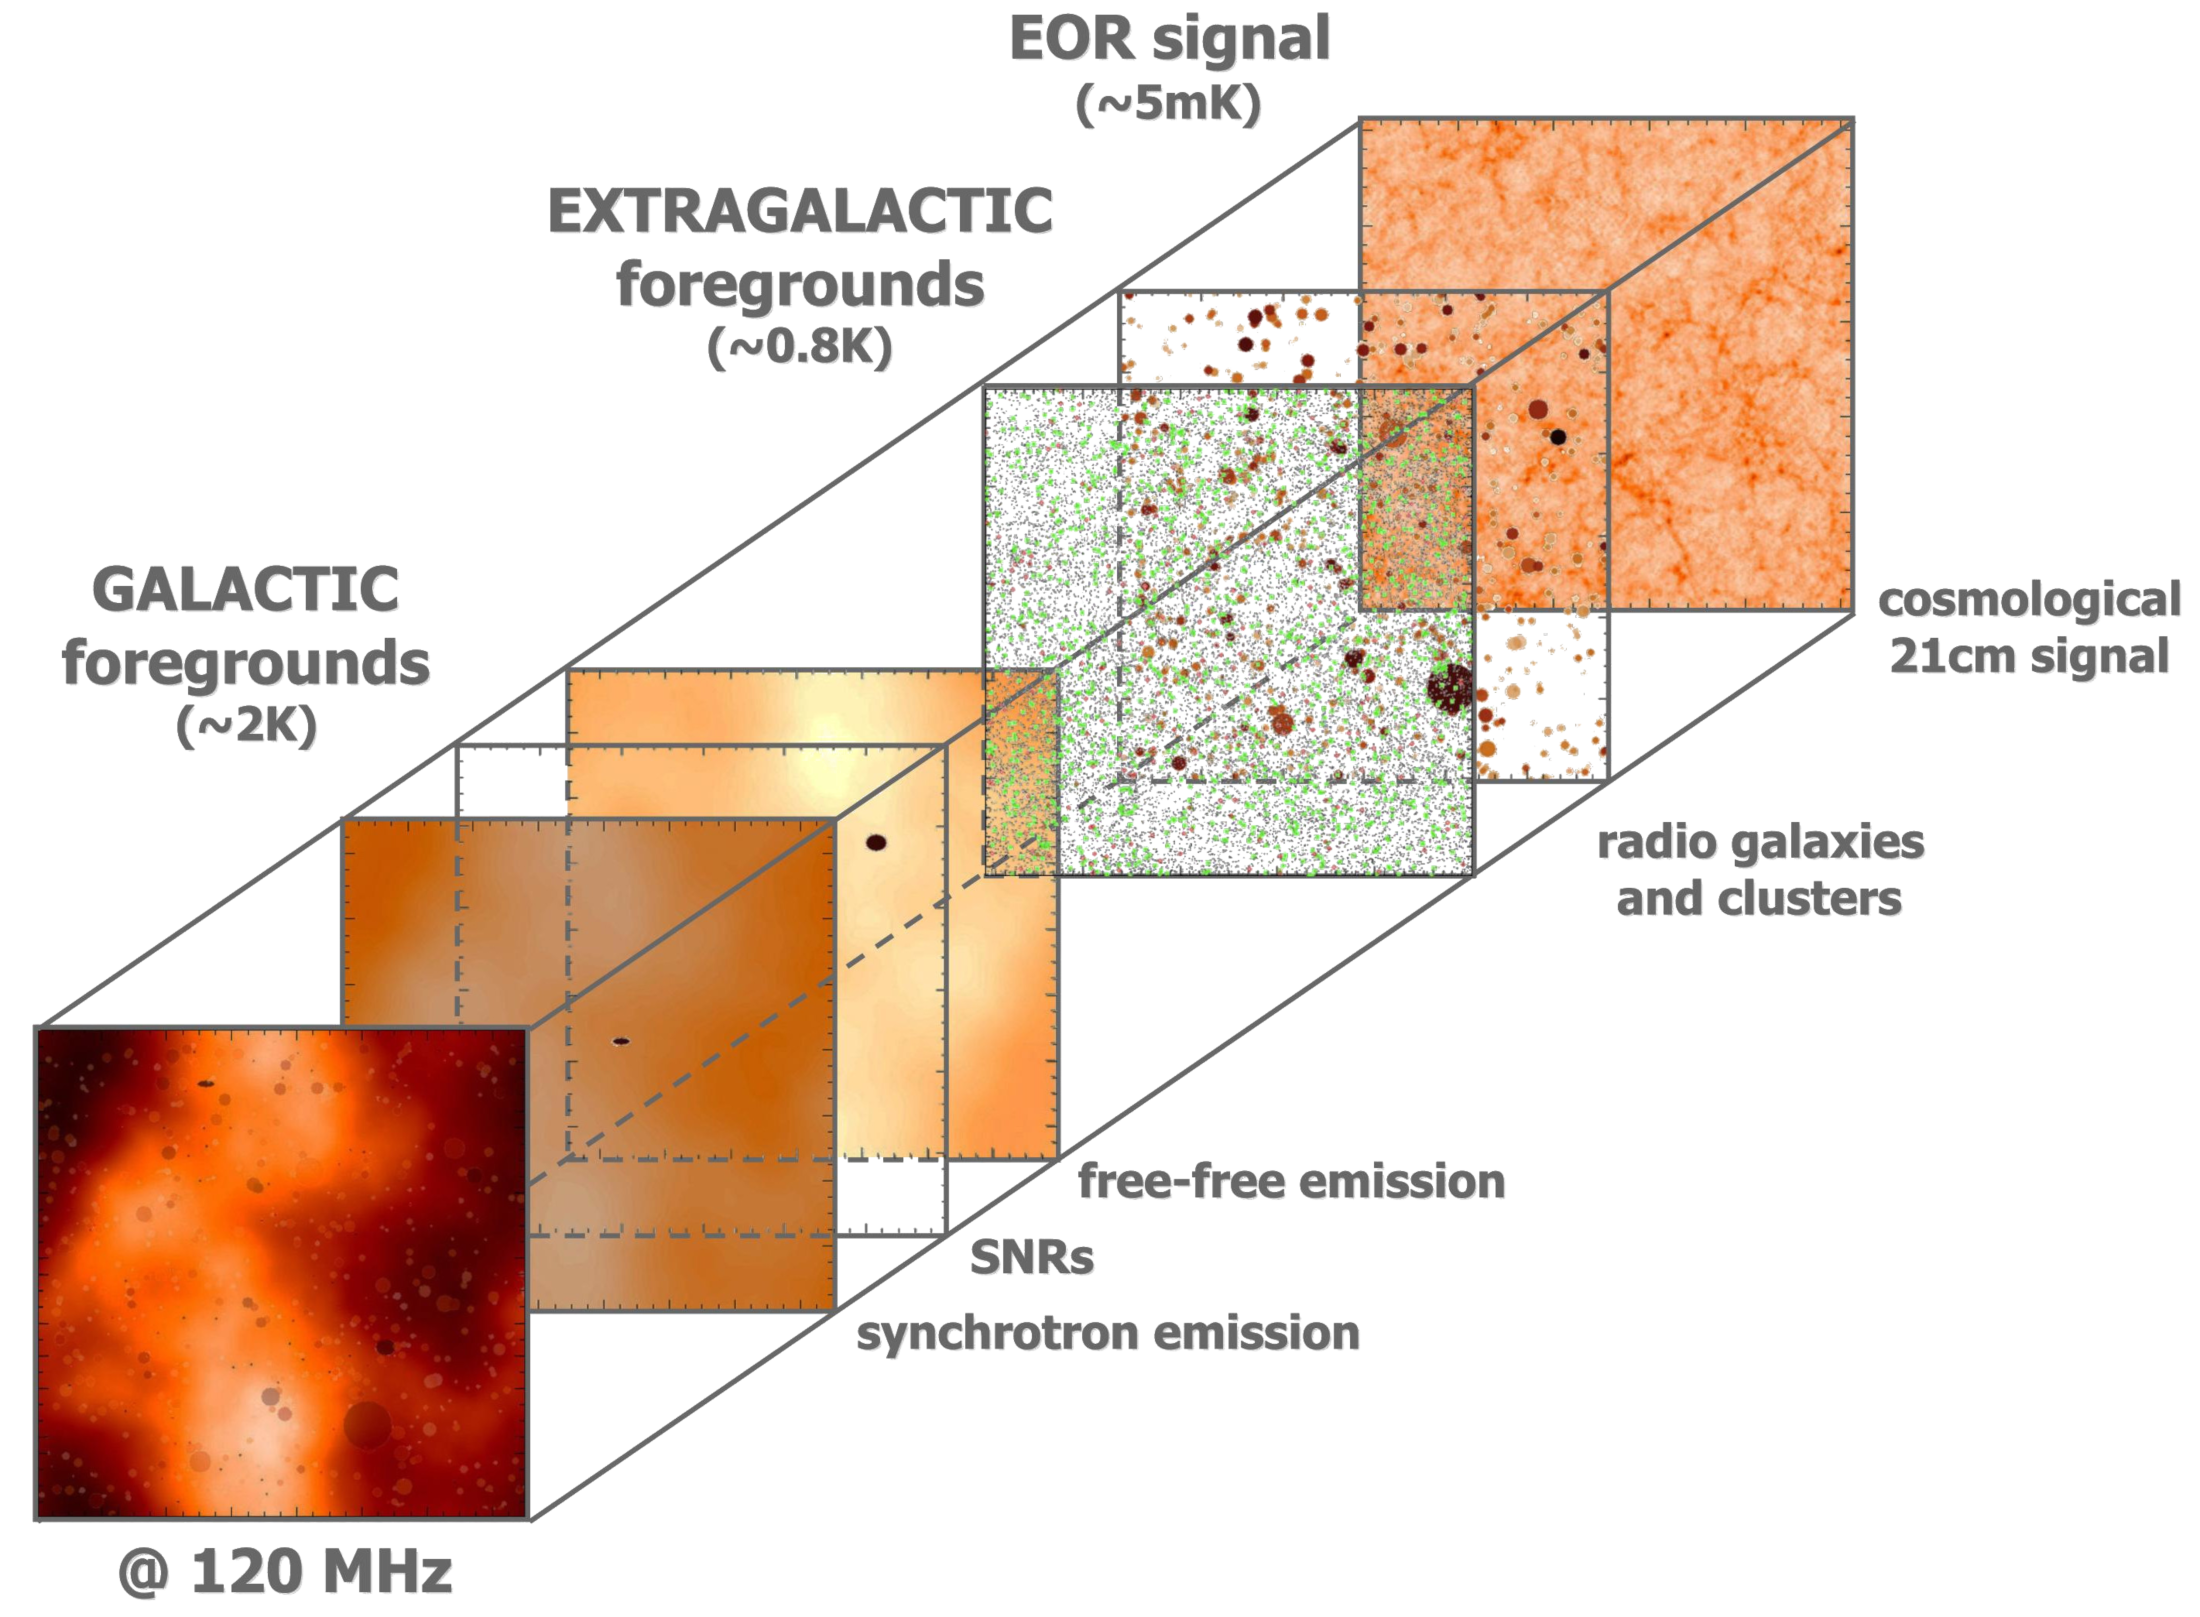
\includegraphics[width=0.7\textwidth]{eor-foregrounds}
  \end{figure}

  \blfootnote{图片来源: \cite{zaroubi2013}}
\end{frame}

%............
\begin{frame}{本文研究内容}
  \begin{alertblock}{1. 射电晕建模的改进以及对 EoR 探测影响的评估}
    \begin{itemize}
      \item 星系团射电晕:常见的射电展源,
        尺度较大,形态相对复杂,数目较多
      \item 已有研究不多,且比较粗糙,值得深入探讨
      \item 课题组研究星系团的丰富经验
    \end{itemize}
  \end{alertblock}

  \begin{alertblock}{2. EoR 信号分离算法的研发}
    \begin{itemize}
      \item 利用上述改进的模拟结果,研究仪器波束效应对 EoR 信号分离的影响
      \item 基于深度学习研发 EoR 信号分离算法,尝试克服波束效应的影响
    \end{itemize}
  \end{alertblock}
\end{frame}

%............
\begin{frame}{本文框架}
  \begin{figure}
    \makebox[\textwidth][c]{%
      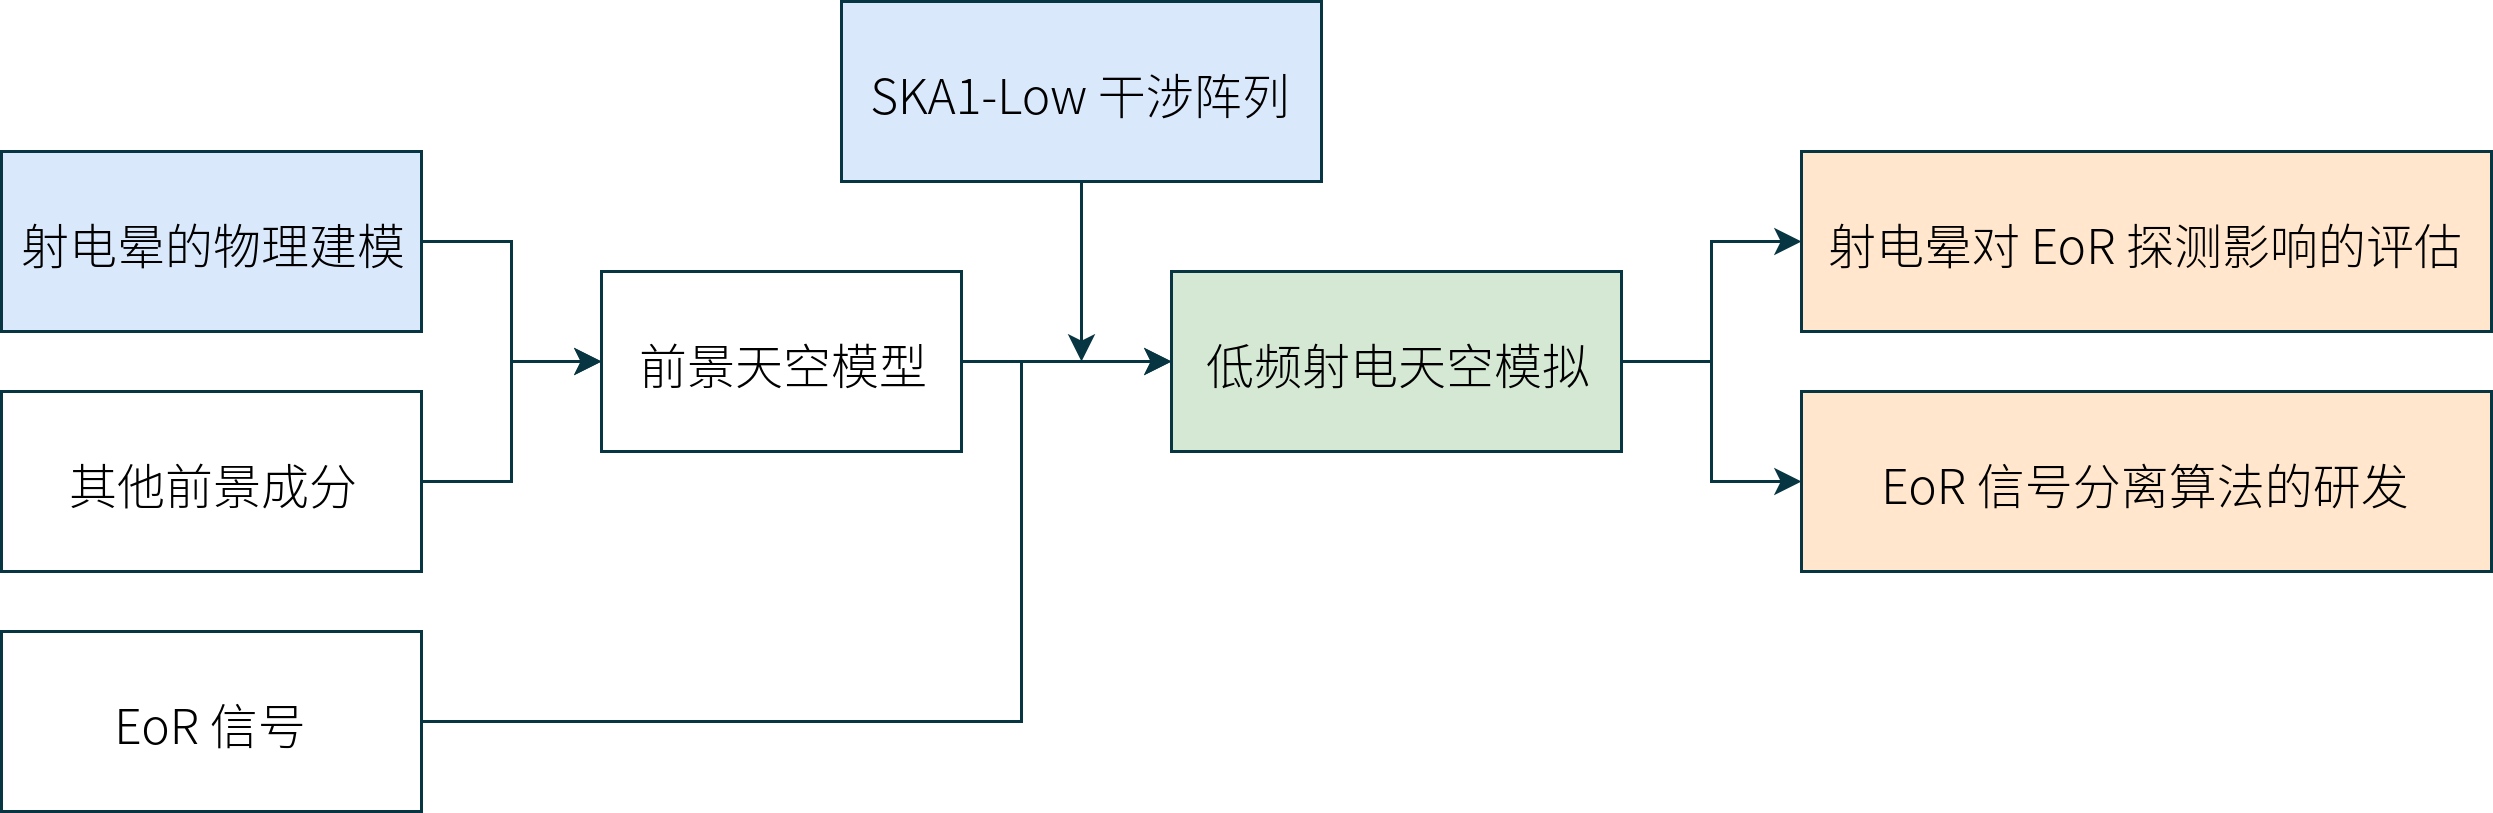
\includegraphics[width=1.1\textwidth]{flow-thesis}}
  \end{figure}
\end{frame}


%=====================================================================
\section{低频射电天空建模的改进}

\begin{frame}
  \begin{block}{主要流程}
    \vspace{-1ex}
    \begin{figure}
      \makebox[\textwidth][c]{%
        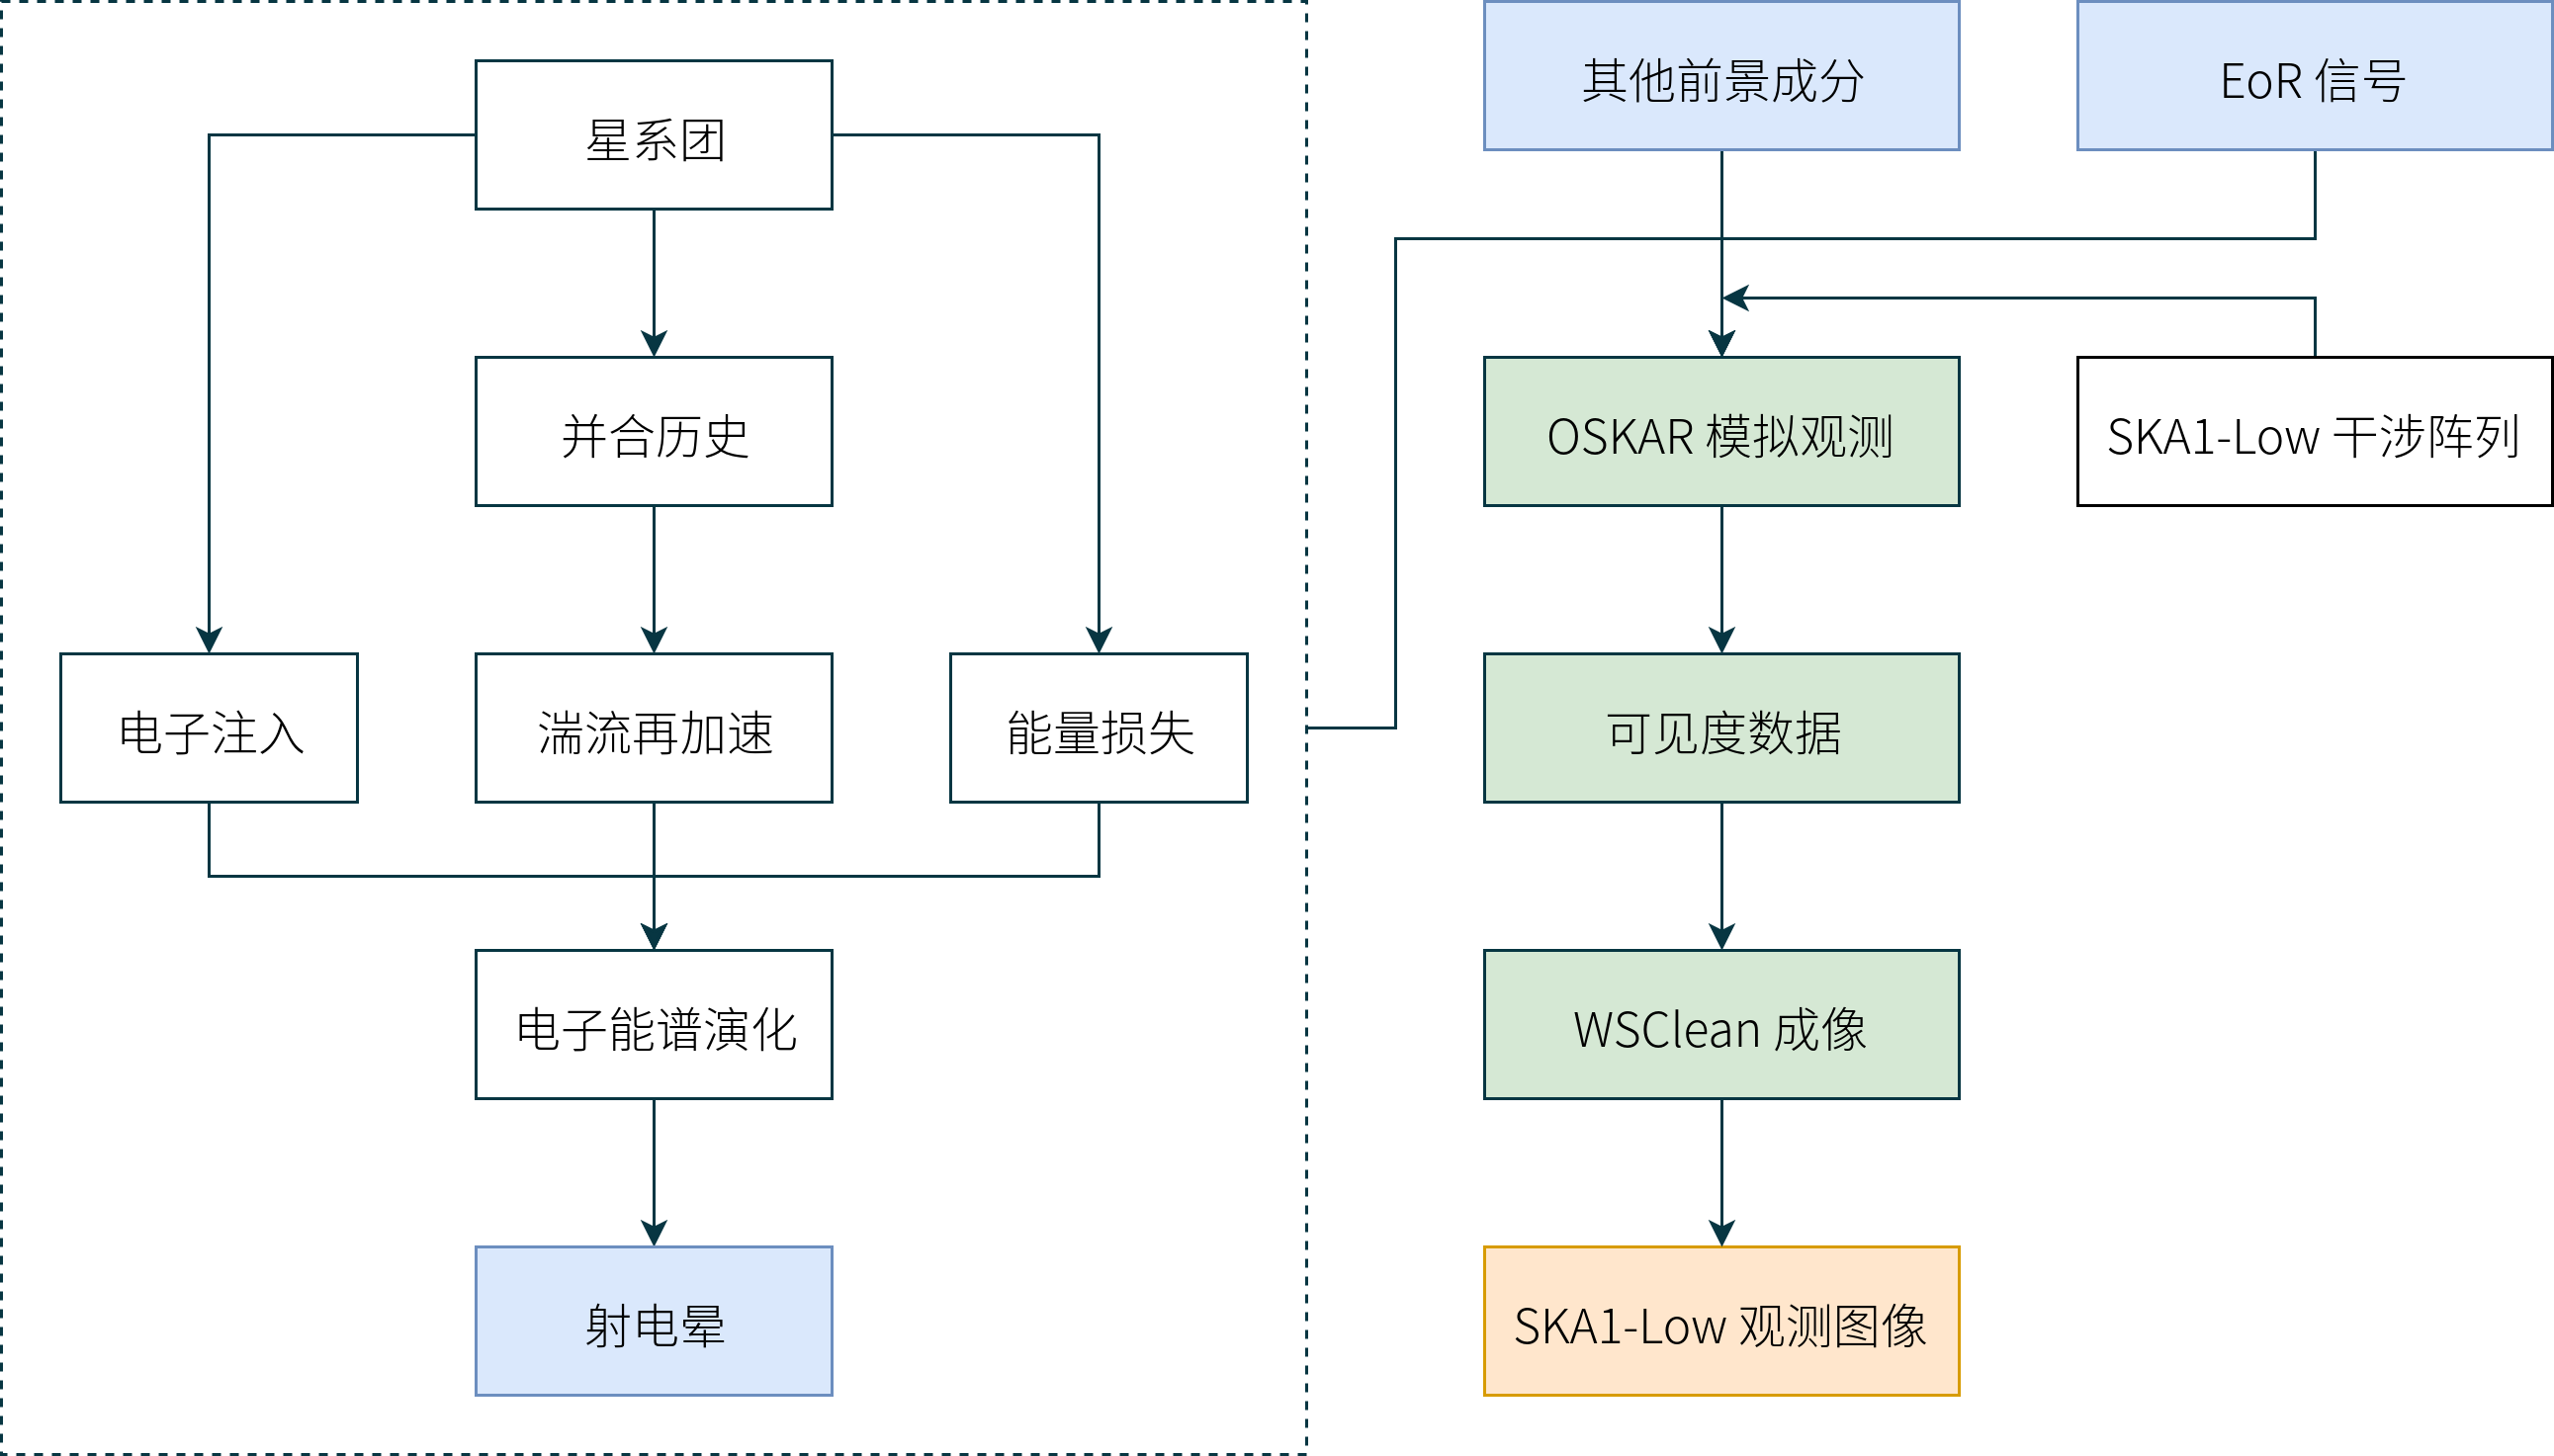
\includegraphics[width=1.1\textwidth]{flow-simulation}}
    \end{figure}
  \end{block}
\end{frame}

%---------------------------------------------------------------------
\subsection{射电晕的建模及天图模拟}

%............
\begin{frame}{2.1 射电晕的建模及天图模拟}
  \begin{alertblock}{主要步骤}
    \begin{enumerate}
      \item 模拟星系团的质量和红移分布
      \item 模拟星系团的并合历史
      \item 计算高能电子能谱的时间演化
      \item 计算射电晕的性质并生成图像
    \end{enumerate}
  \end{alertblock}
\end{frame}

%............
\begin{frame}[subsec]
  \frametitle{(1) 星系团的质量和红移分布}
  \begin{columns}[t,onlytextwidth]
    \column{0.48\textwidth}
    \begin{itemize}
      \item Press--Schechter (PS) 理论:
        任意红移时刻星系团的质量分布
      \item 从 PS 质量函数随机生成 $(M, z)$ 样本
    \end{itemize}

    \column{0.5\textwidth}
    \begin{figure}
      \centering
      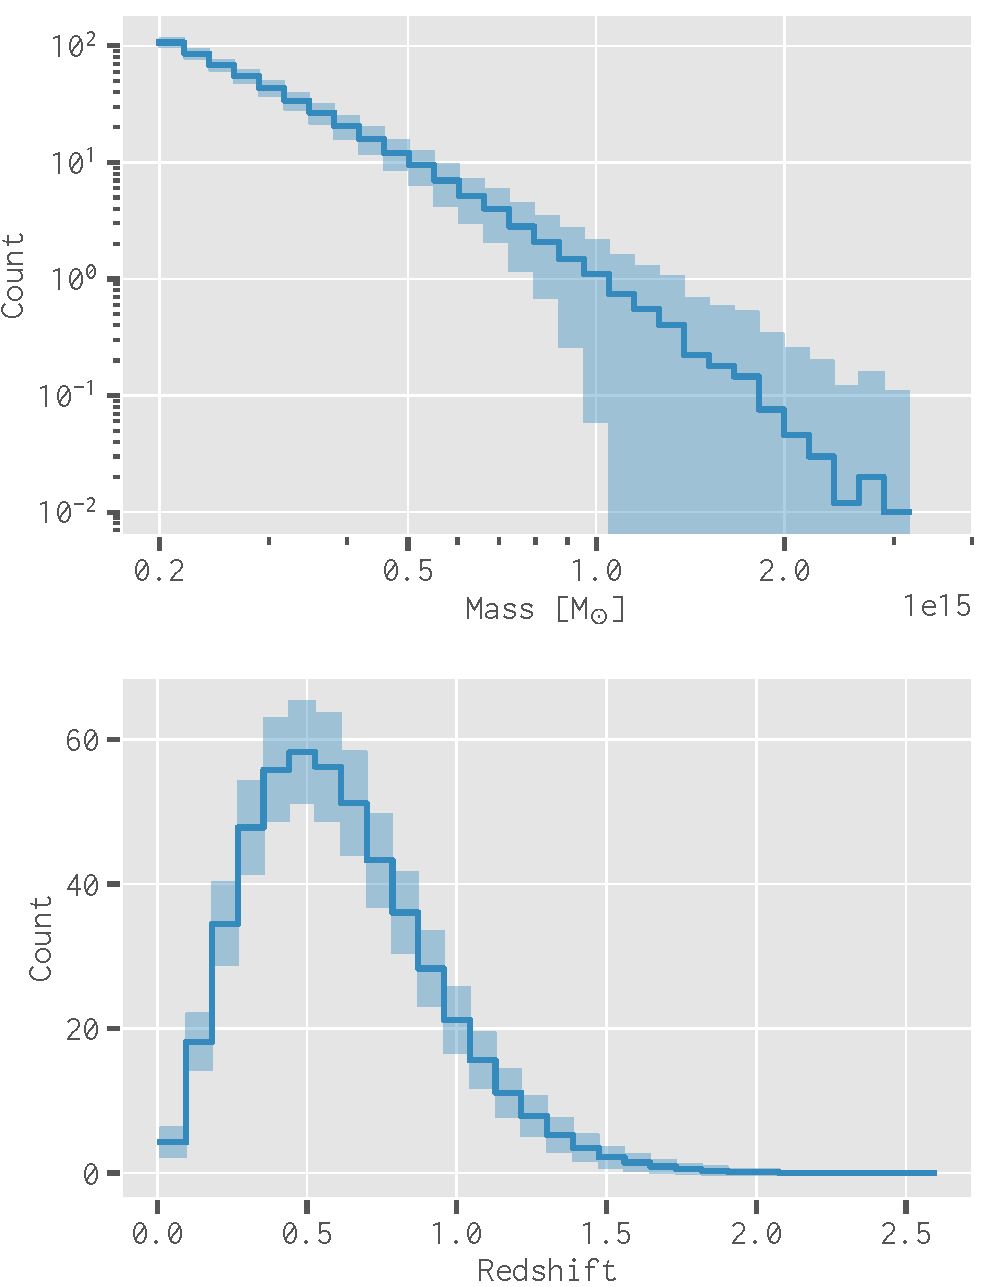
\includegraphics[width=\columnwidth]{mass-z-dist}
    \end{figure}
  \end{columns}
\end{frame}

%............
\begin{frame}[subsec]
  \frametitle{(2) 星系团的并合历史}
  \begin{columns}[t,onlytextwidth]
    \column{0.48\textwidth}
    \begin{itemize}
      \item 扩展 PS 理论:星系团的前身质量的条件概率分布
      \item Monte Carlo 模拟并合树
    \end{itemize}

    \column{0.5\textwidth}
    \begin{figure}
      \centering
      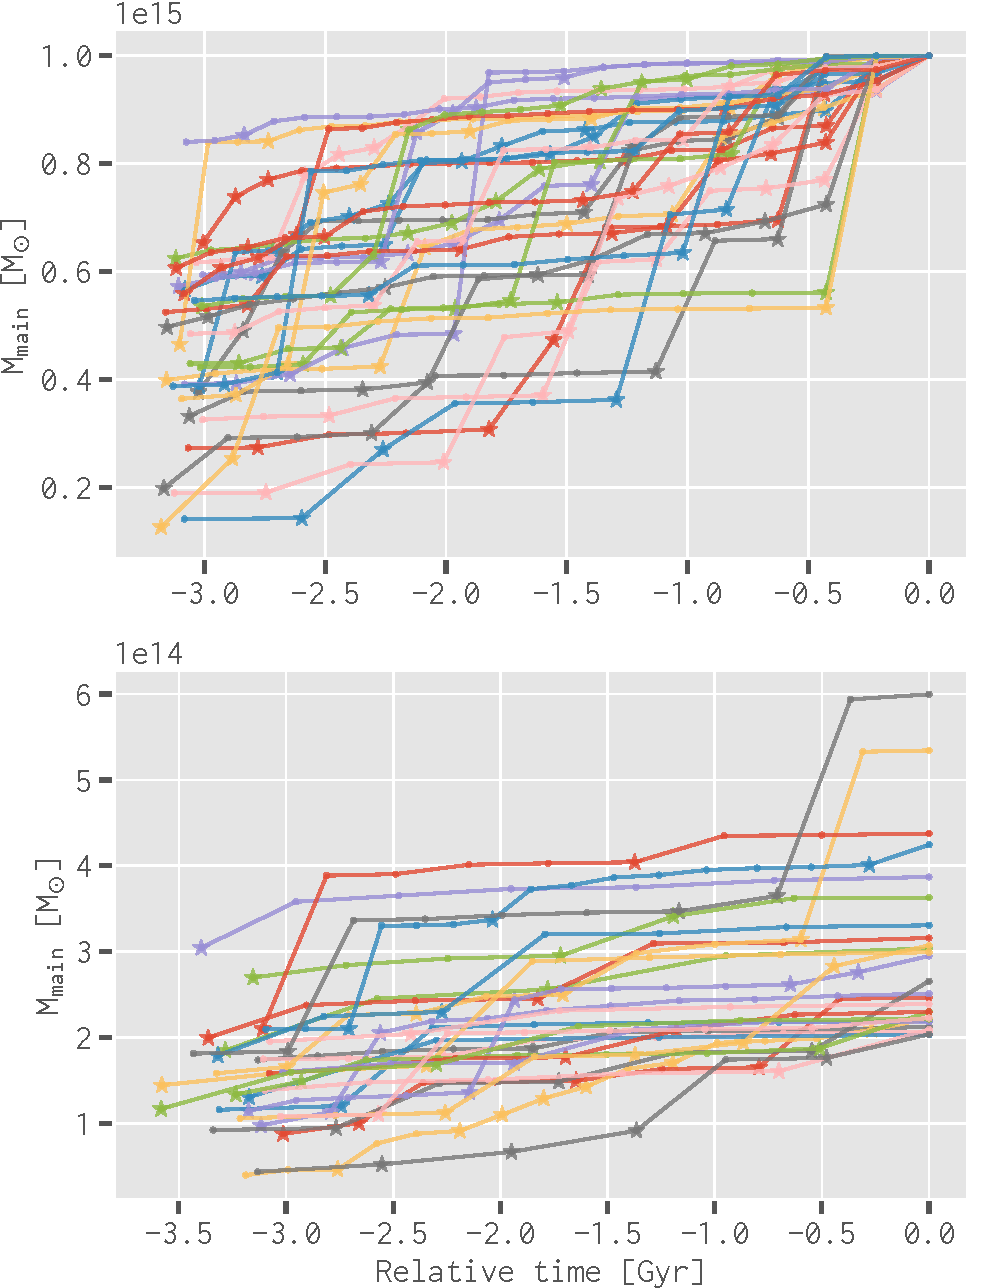
\includegraphics[width=\columnwidth]{merging-history}
    \end{figure}
  \end{columns}
\end{frame}

%............
\begin{frame}[subsec]
  \frametitle{(3) 高能电子的演化模型}
  \begin{itemize}
    \item 构建演化模型:
      \begin{itemize}
        \item 电子注入过程
        \item 并合湍流再加速过程
        \item 能量损失过程
      \end{itemize}
    \item 数值求解 Fokker--Planck 方程:
      \begin{multline}
        \pdiff{n_e(\gamma, t)}{t} =
          \pdiff{}{\gamma} \left[ n_e(\gamma, t) \left(
            \left| \diff{\gamma}{t} \right| -
            \frac{2}{\gamma} D_{\gamma\gamma}(\gamma, t) \right) \right] + \\
          \pdiff{}{\gamma} \left[
          D_{\gamma\gamma} \pdiff{n_e(\gamma, t)}{\gamma} \right]
          + Q_e(\gamma, t)
      \end{multline}
  \end{itemize}
\end{frame}

%............
\begin{frame}[t]
  \begin{block}{湍流再加速示例
    {\normalfont(1\,$\oplus$\,\SI{0.6e15}{\solarmass},
      \SIrange{10.3}{11.8}{\Gyr})}
  }
    \begin{figure}
      \centering\footnotesize
      \hspace{2.5em} 电子能谱 \hspace{9em} 辐射频谱 \\
      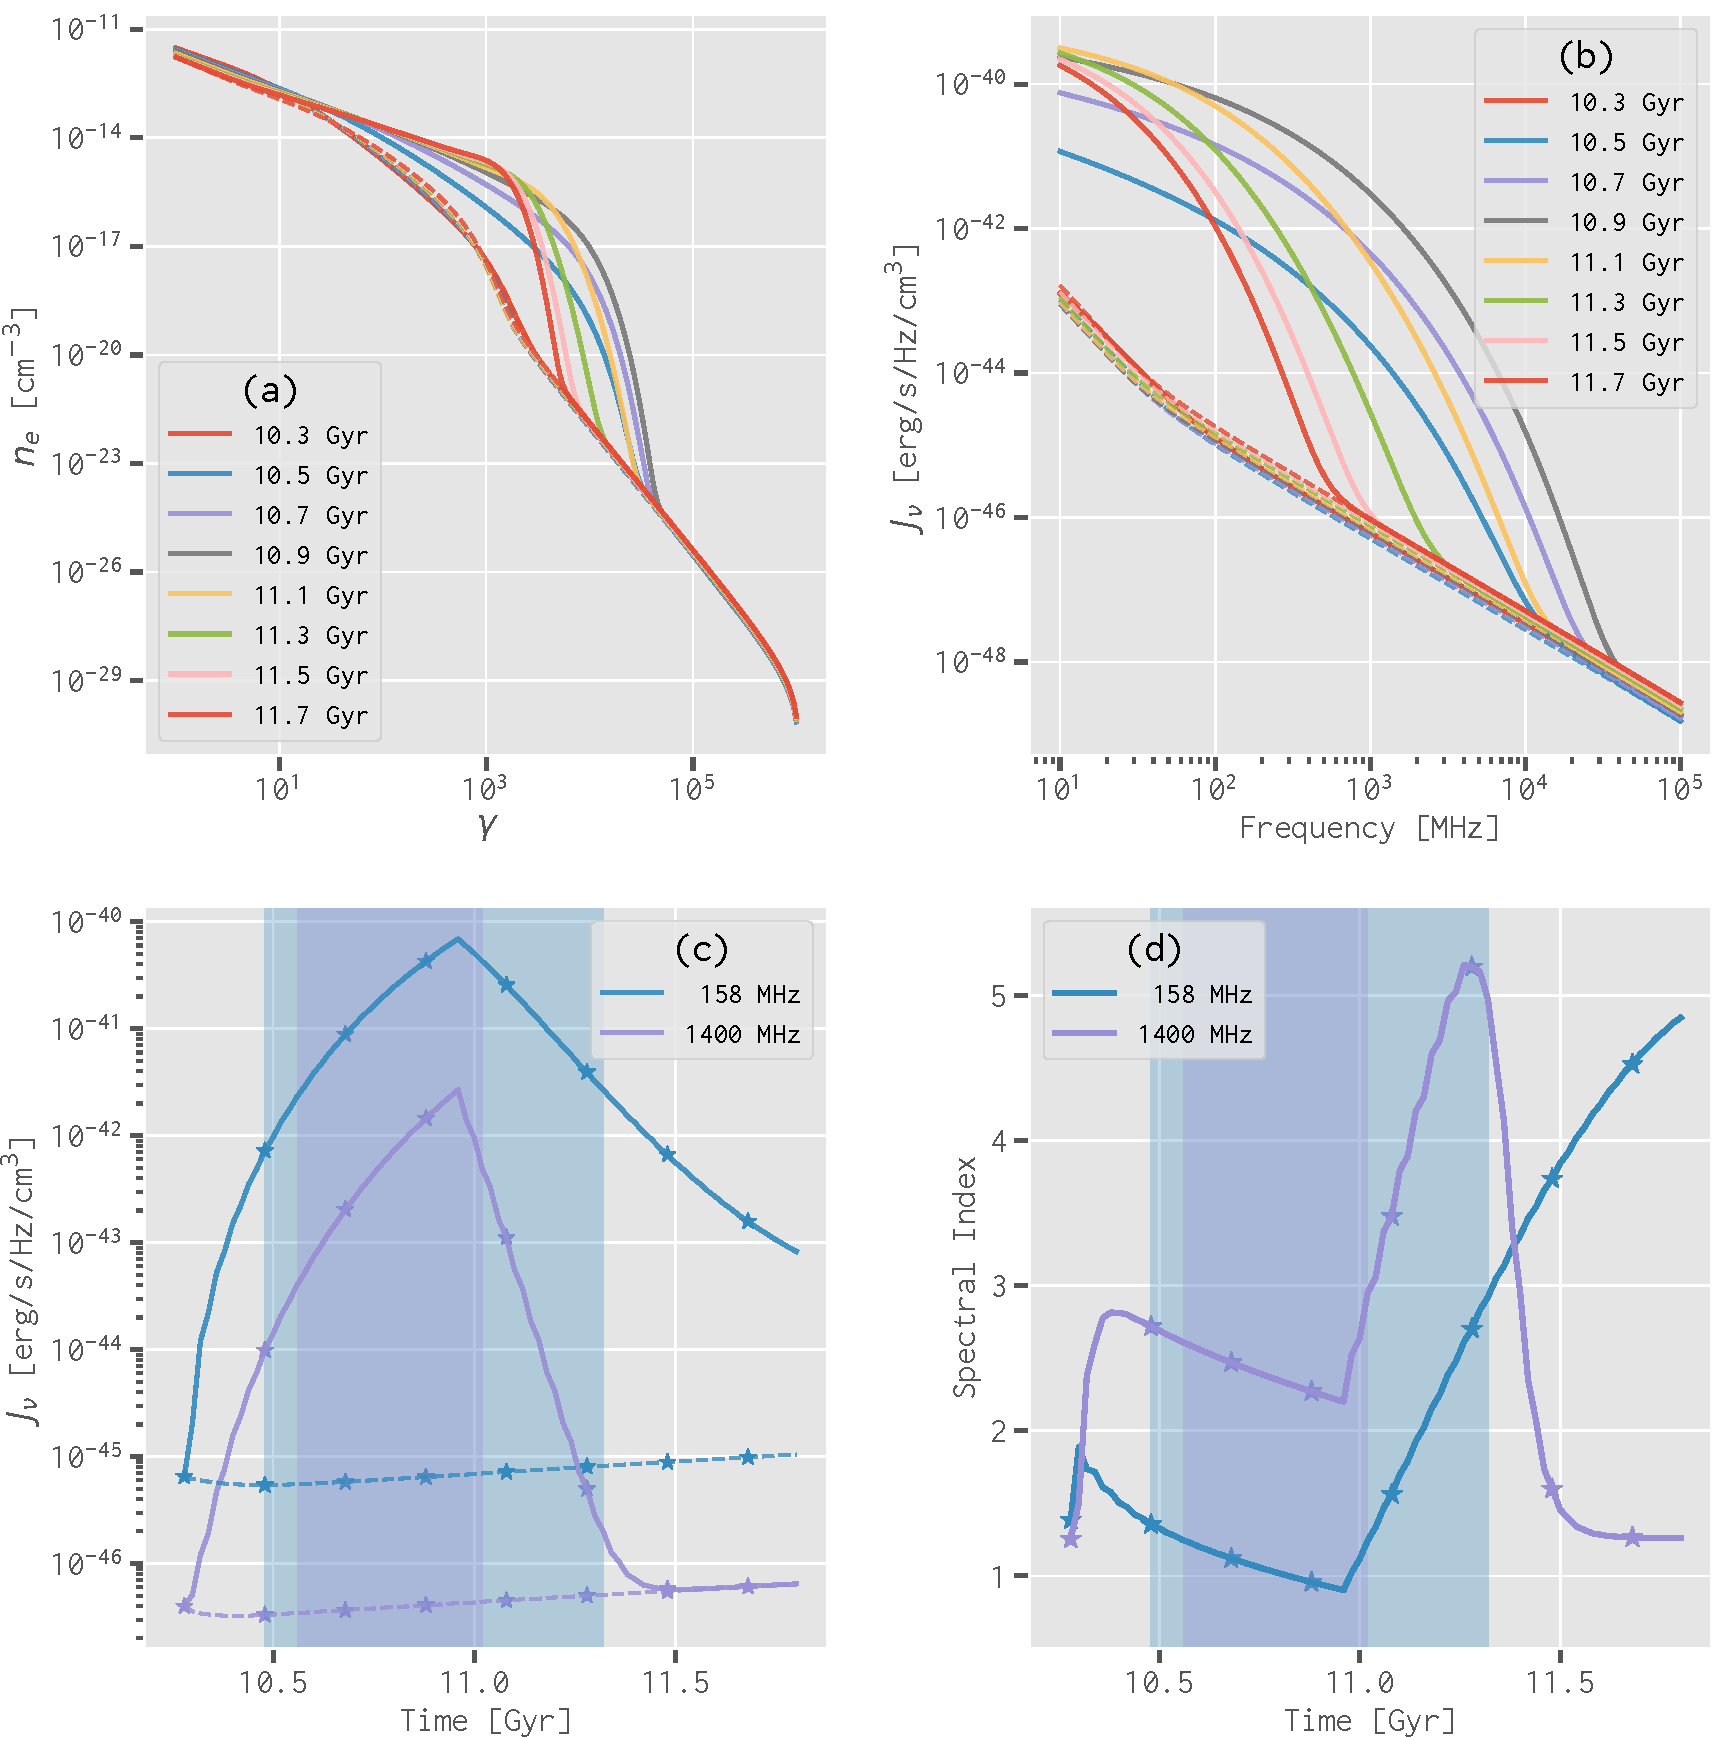
\includegraphics[width=0.8\textwidth]{spec-evo-example} \\
      \hspace{2.5em} 同步辐射发射率 \hspace{7em} 同步辐射谱指数
    \end{figure}
  \end{block}
\end{frame}

%............
\begin{frame}[subsec]
  \frametitle{(4) 射电晕天图生成}
  \begin{columns}[t,onlytextwidth]
    \column{0.4\textwidth}
    \vspace{-1ex}
    \begin{table}
      \centering\small
      \begin{tabular}{cc}
        \toprule
        参数 & 取值 \\
        \midrule
        频带 & 120--128\,MHz \\
            & 154--162\,MHz \\
            & 192--200\,MHz \\
        带宽 & \SI{8}{\MHz} \\
        频率分辨率 & \SI{160}{\kHz} \\
        天区大小 & \SI{10 x 10}{\degree} \\
        图像大小 & \num{1800 x 1800} \\
        像素大小 & \SI{20}{\arcsecond} \\
        \bottomrule
      \end{tabular}
    \end{table}

    \column{0.55\textwidth}
    \begin{figure}
      \centering\footnotesize
      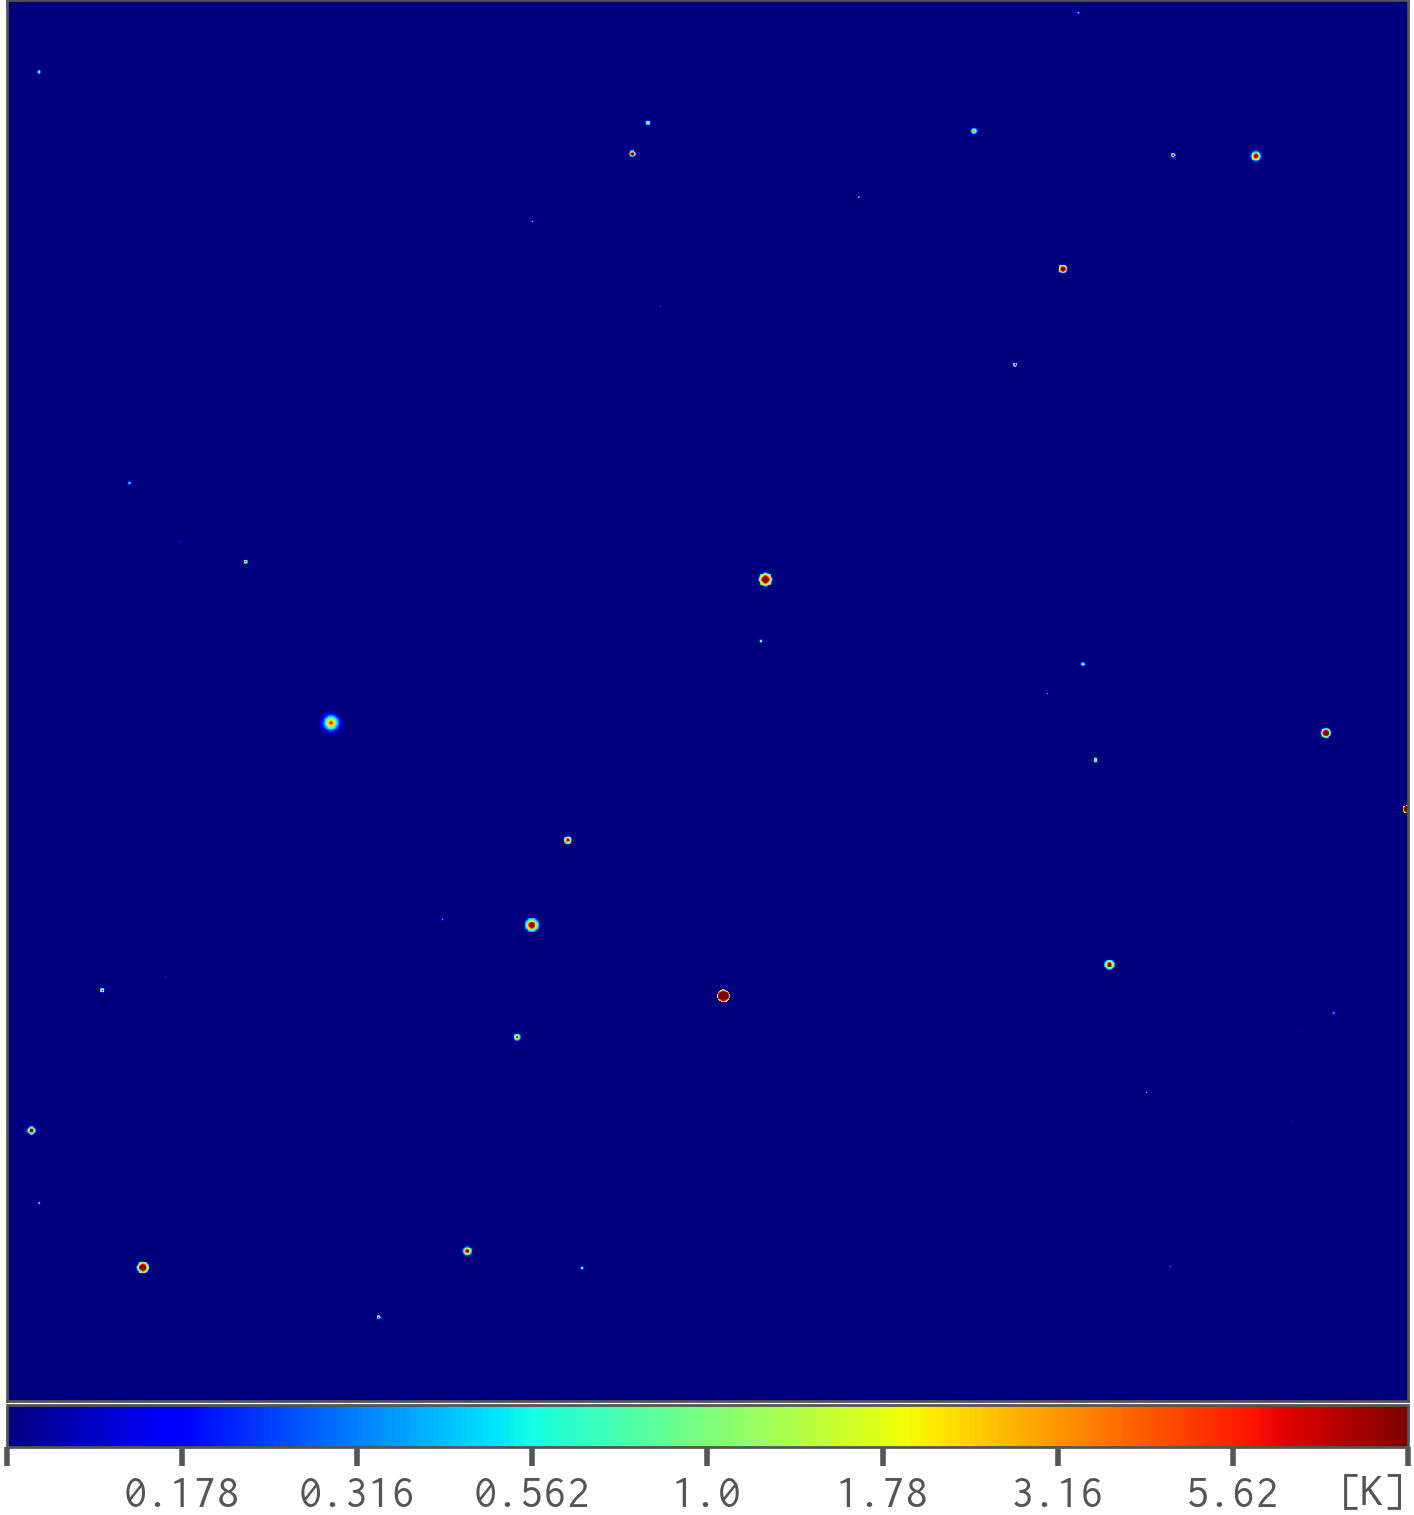
\includegraphics[width=\columnwidth]{skymap-halos-f158}
      射电晕 \SI{158}{\MHz} 天图示例
    \end{figure}
  \end{columns}
\end{frame}

%---------------------------------------------------------------------
\subsection{其他前景成分的天图模拟}

%............
\begin{frame}{2.2 其他前景成分的天图模拟}
  \begin{alertblock}{银河系同步辐射}
    \begin{itemize}
      \item 以 Haslam \SI{408}{\MHz} 全天图为模板向低频外延
      \item 考虑了谱指数随天空位置的变化
    \end{itemize}
  \end{alertblock}

  \begin{alertblock}{银河系自由—自由辐射}
    \vspace{1ex}
    从 Hα 辐射导出,修正了尘埃吸收
  \end{alertblock}

  \begin{alertblock}{河外点源}
    \begin{itemize}
      \item 继承自我们之前的一项工作:\cite{wang2010}
      \item 模拟了 4 类点源:
        (1) FR I 型和 II 型射电星系、
        (2) 恒星形成星系、
        (3) 射电宁静 AGN、
        (4) GHz 倒转谱和致密陡谱 AGN
    \end{itemize}
  \end{alertblock}
\end{frame}

%............
\begin{frame}[c]
  \begin{alertblock}{\SI{158}{\MHz} 天图示例}
  \end{alertblock}
  \begin{columns}
    \column{0.37\textwidth}
    \begin{figure}
      \centering\footnotesize
      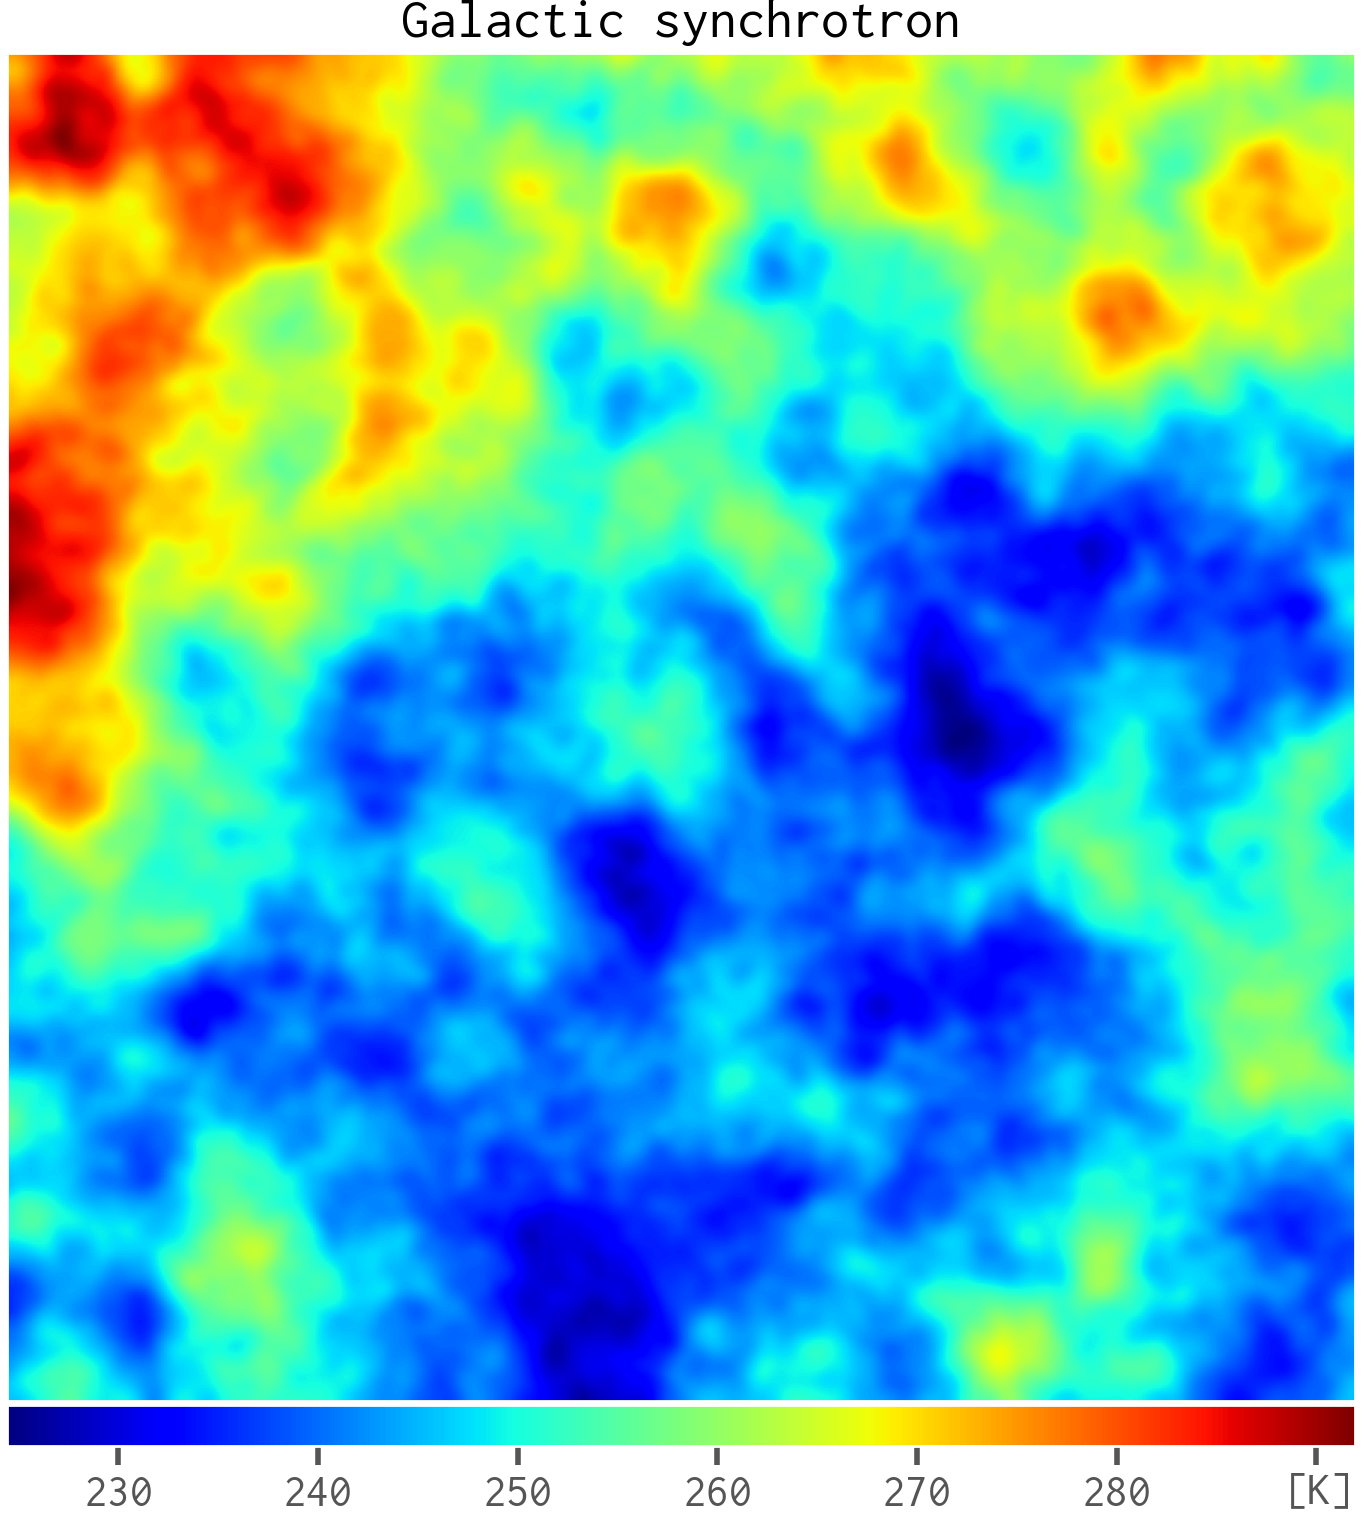
\includegraphics[width=\columnwidth]{skymap-gsyn-f158}
      银河系同步辐射
    \end{figure}

    \column{0.37\textwidth}
    \begin{figure}
      \centering\footnotesize
      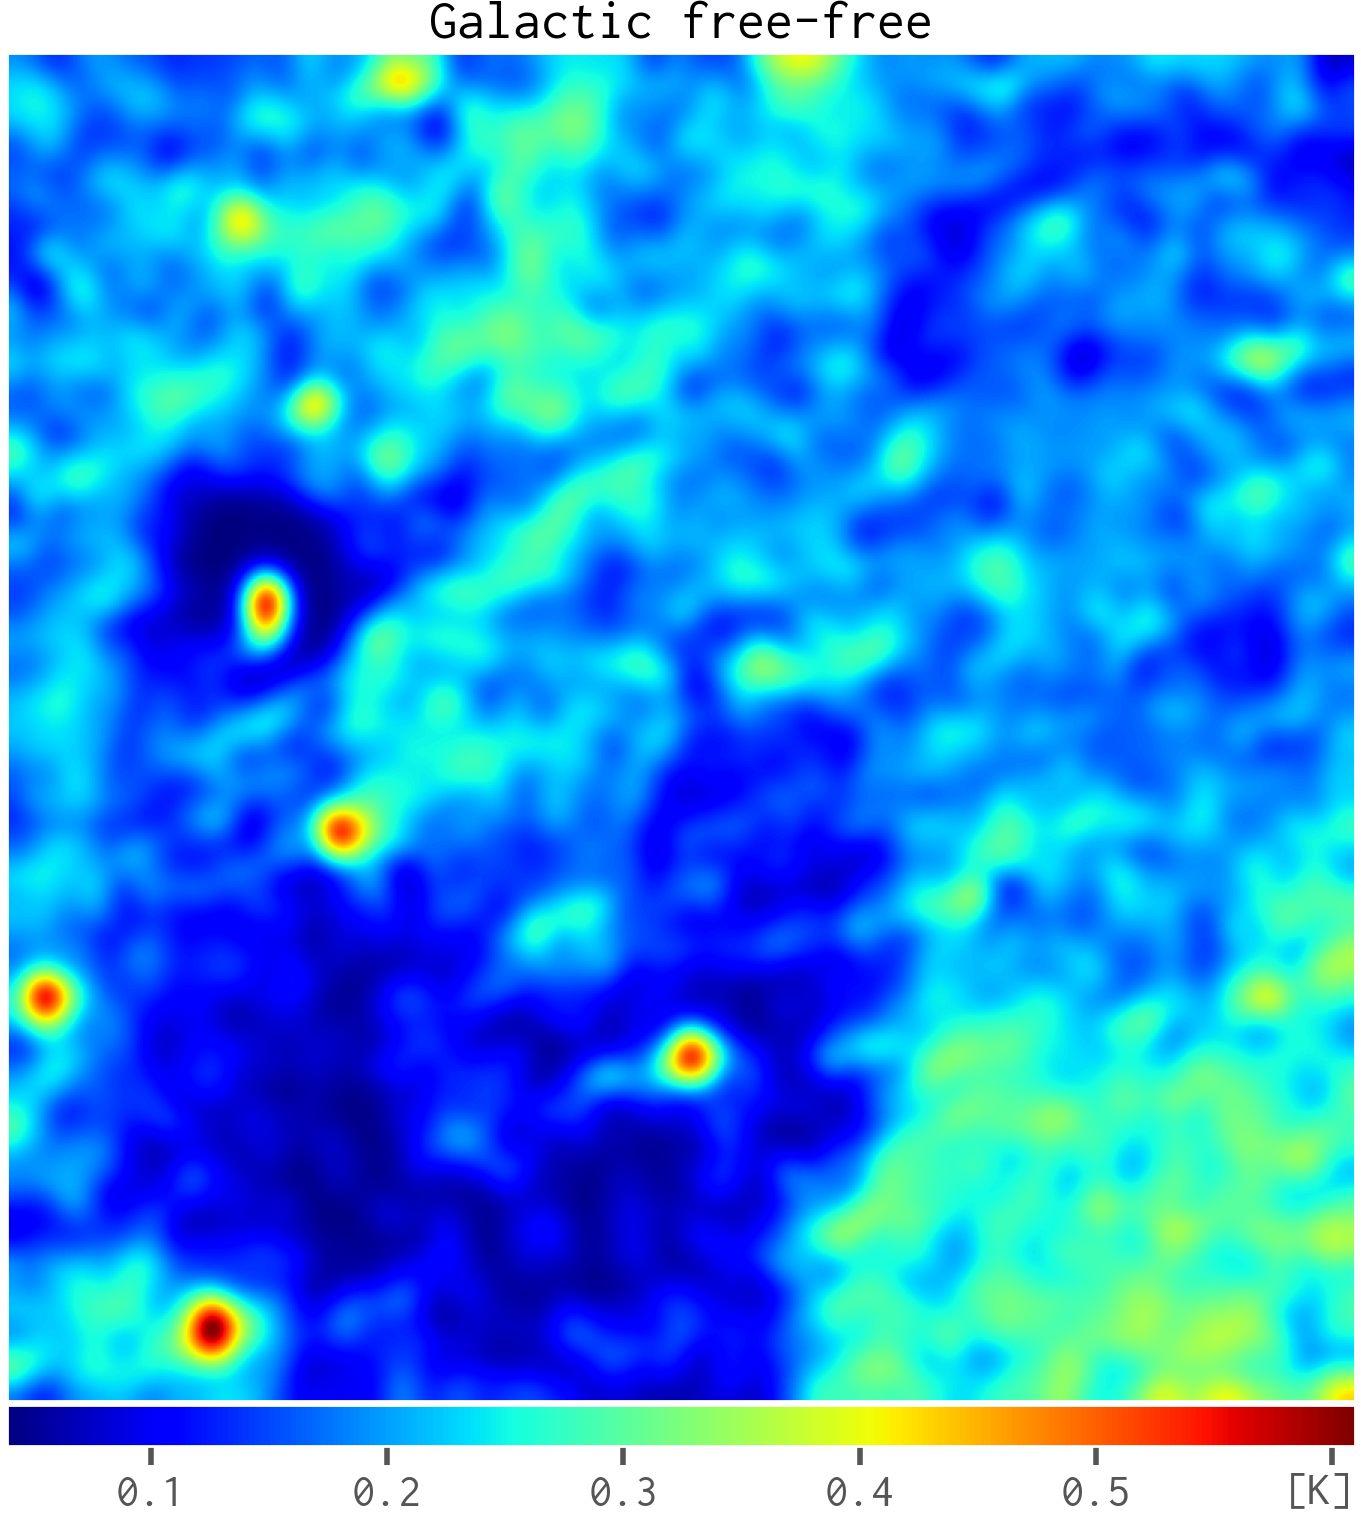
\includegraphics[width=\columnwidth]{skymap-gff-f158}
      银河系自由—自由辐射
    \end{figure}

    \column{0.37\textwidth}
    \begin{figure}
      \centering\footnotesize
      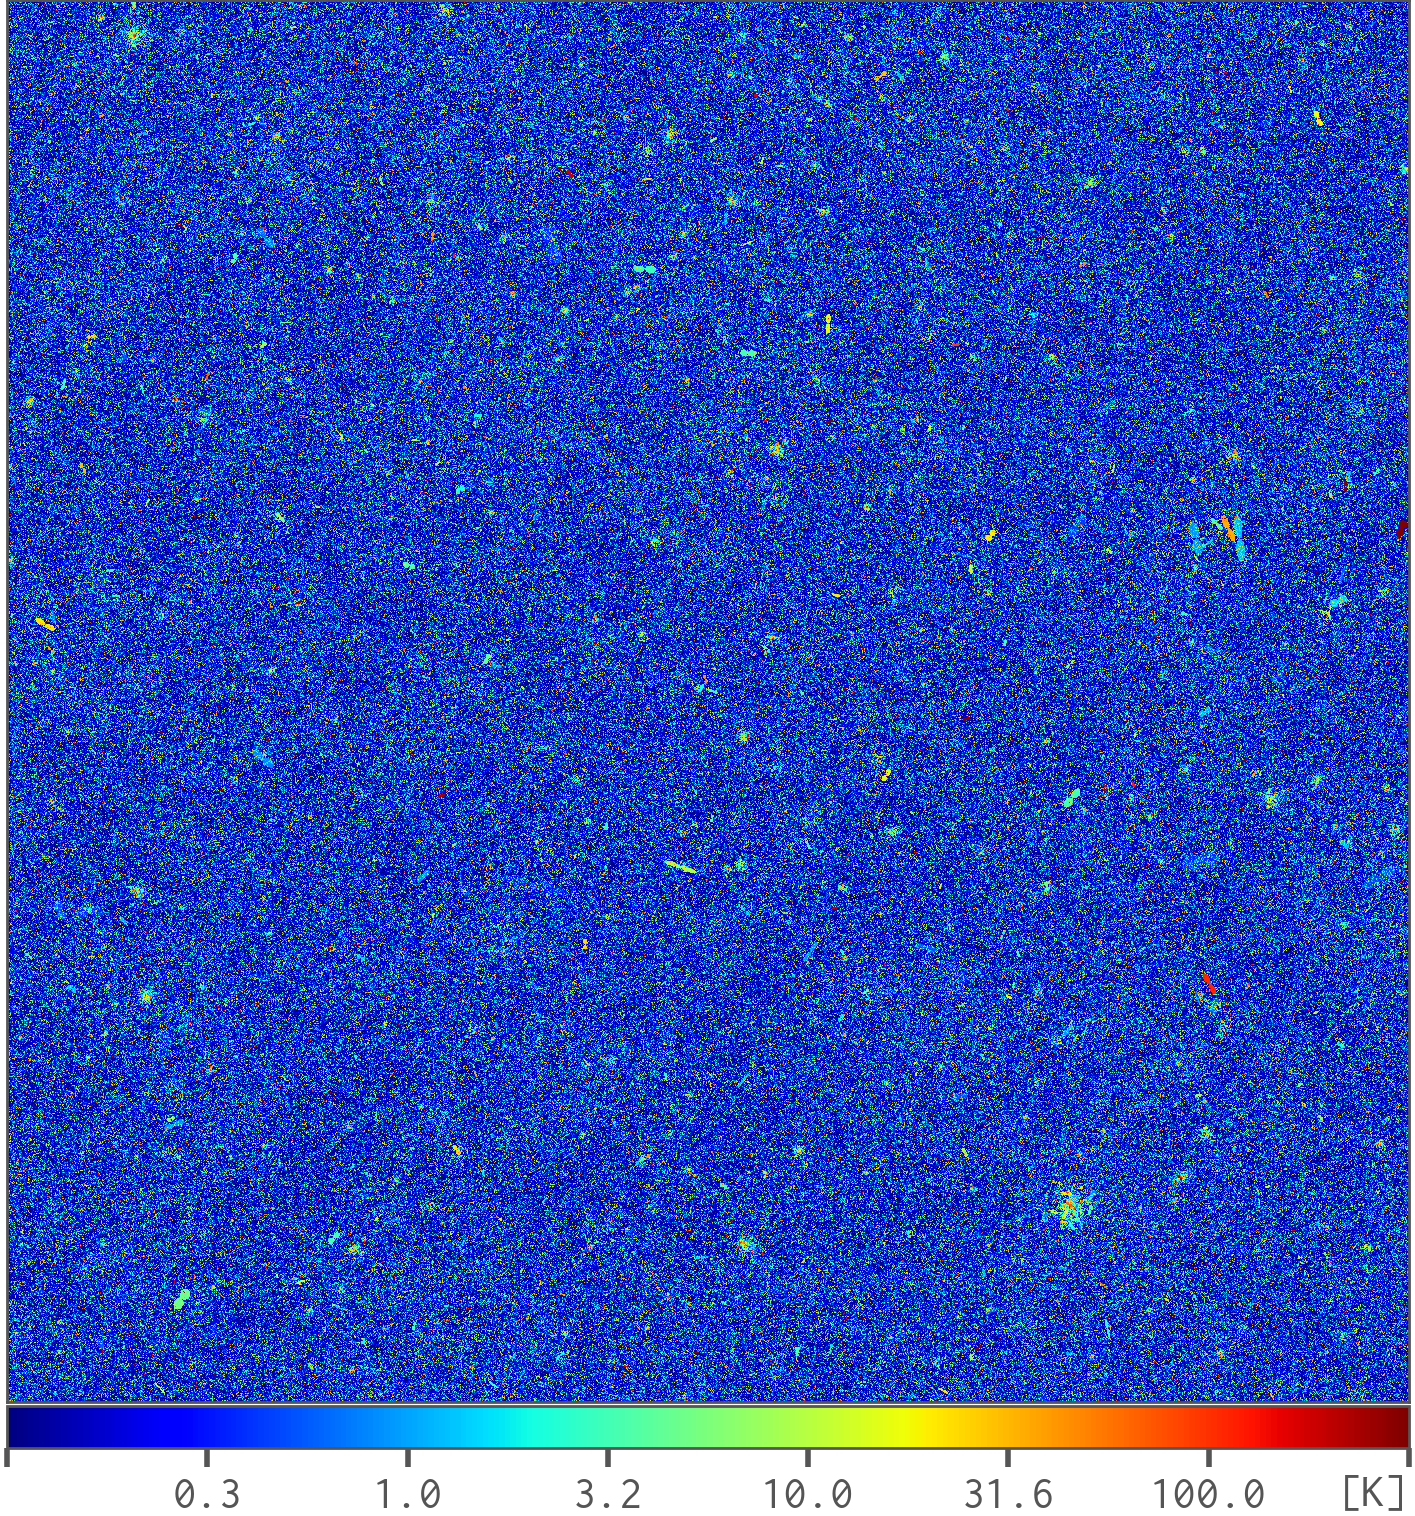
\includegraphics[width=\columnwidth]{skymap-ptrsrc-f158}
      河外点源
    \end{figure}
  \end{columns}
\end{frame}

%---------------------------------------------------------------------
\subsection{EoR 信号天图模拟}

%............
\begin{frame}{2.3 EoR 信号天图模拟}
  \begin{columns}[t,onlytextwidth]
    \column{0.48\textwidth}
    \begin{itemize}
      \item 使用了 \href{http://homepage.sns.it/mesinger/EOS.html}{\textit{Evolution Of 21\,cm Structure}}
        项目公开的 EoR 模拟数据
      \item 提取所需红移(即频率)处的图像切片,平铺和缩放,
        与前景天图的大小和分辨率一致
    \end{itemize}

    \column{0.5\textwidth}
    \begin{figure}
      \centering\footnotesize
      \includegraphics[width=\columnwidth]{skymap-eor-f158}
      EoR 信号 \SI{158}{\MHz} 天图
    \end{figure}
  \end{columns}
\end{frame}

%---------------------------------------------------------------------
\subsection{SKA1-Low 观测图像的模拟}

%............
\begin{frame}{2.4 SKA1-Low 观测图像的模拟}
  \begin{alertblock}{主要步骤}
  \begin{enumerate}
    \item 采用 \alert{SKA1-Low 阵列布局} (2016-05-31)
    \item 使用 \href{https://github.com/OxfordSKA/OSKAR}{\texttt{OSKAR}}
      模拟天图的\alert{可见度数据}
    \item 使用 \href{https://sourceforge.net/projects/wsclean/}{\texttt{WSClean}}
      从可见度数据生成\alert{观测图像}
  \end{enumerate}
  \end{alertblock}
\end{frame}


%=====================================================================
\section{射电晕辐射对 EoR 信号探测的影响}

\begin{frame}
  \begin{block}{本节提纲}
    \vspace{2ex}
    \tableofcontents[
      sections=\value{section},
      sectionstyle=hide,
    ]
  \end{block}
\end{frame}

%---------------------------------------------------------------------
\subsection{为什么使用功率谱?}

\begin{frame}{3.1 为什么使用功率谱?}
  \begin{itemize}
    \item 对灵敏度、空间分辨率要求较低
    \item 压缩信息,提高 EoR 信号的信噪比
    \item 测量及数据处理相对容易
    \item 分析 EoR 信号和前景干扰的最常用工具
  \end{itemize}
\end{frame}

%............
\begin{frame}[subsec]
  \frametitle{功率谱的计算}
  \begin{columns}[t,onlytextwidth]
    \column{0.55\textwidth}
    \begin{itemize}
      \item \alert{图像立方} $I(\B{\theta}, \nu)$,
        三维 Fourier 变换,得到\alert{三维功率谱} $P(\B{k})$
      \item 按球壳对 $P(\B{k})$ 平均,得到\alert{一维功率谱} $P(k)$
      \item 按 $k_{\parallel}$ 平面内的圆环平均,
        得到\alert{二维功率谱} $P(k_{\perp}, k_{\parallel})$
    \end{itemize}

    \column{0.4\textwidth}
    \begin{figure}
      \centering
      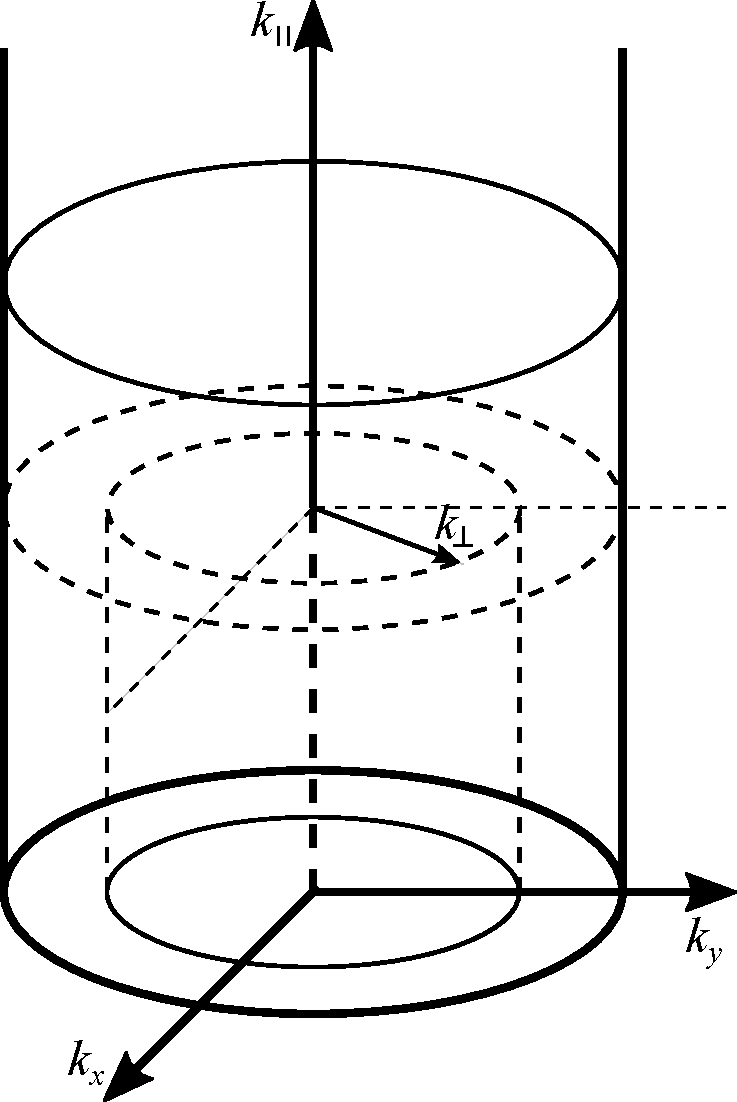
\includegraphics[width=\columnwidth]{ps2d-annuli-diagram}
    \end{figure}
  \end{columns}
\end{frame}

%............
\begin{frame}[t]
  \begin{alertblock}{各成分的二维功率谱
    {\normalfont (\SIrange{154}{162}{\MHz})}
  }
    \vspace{-1ex}
    \begin{figure}
      \centering
      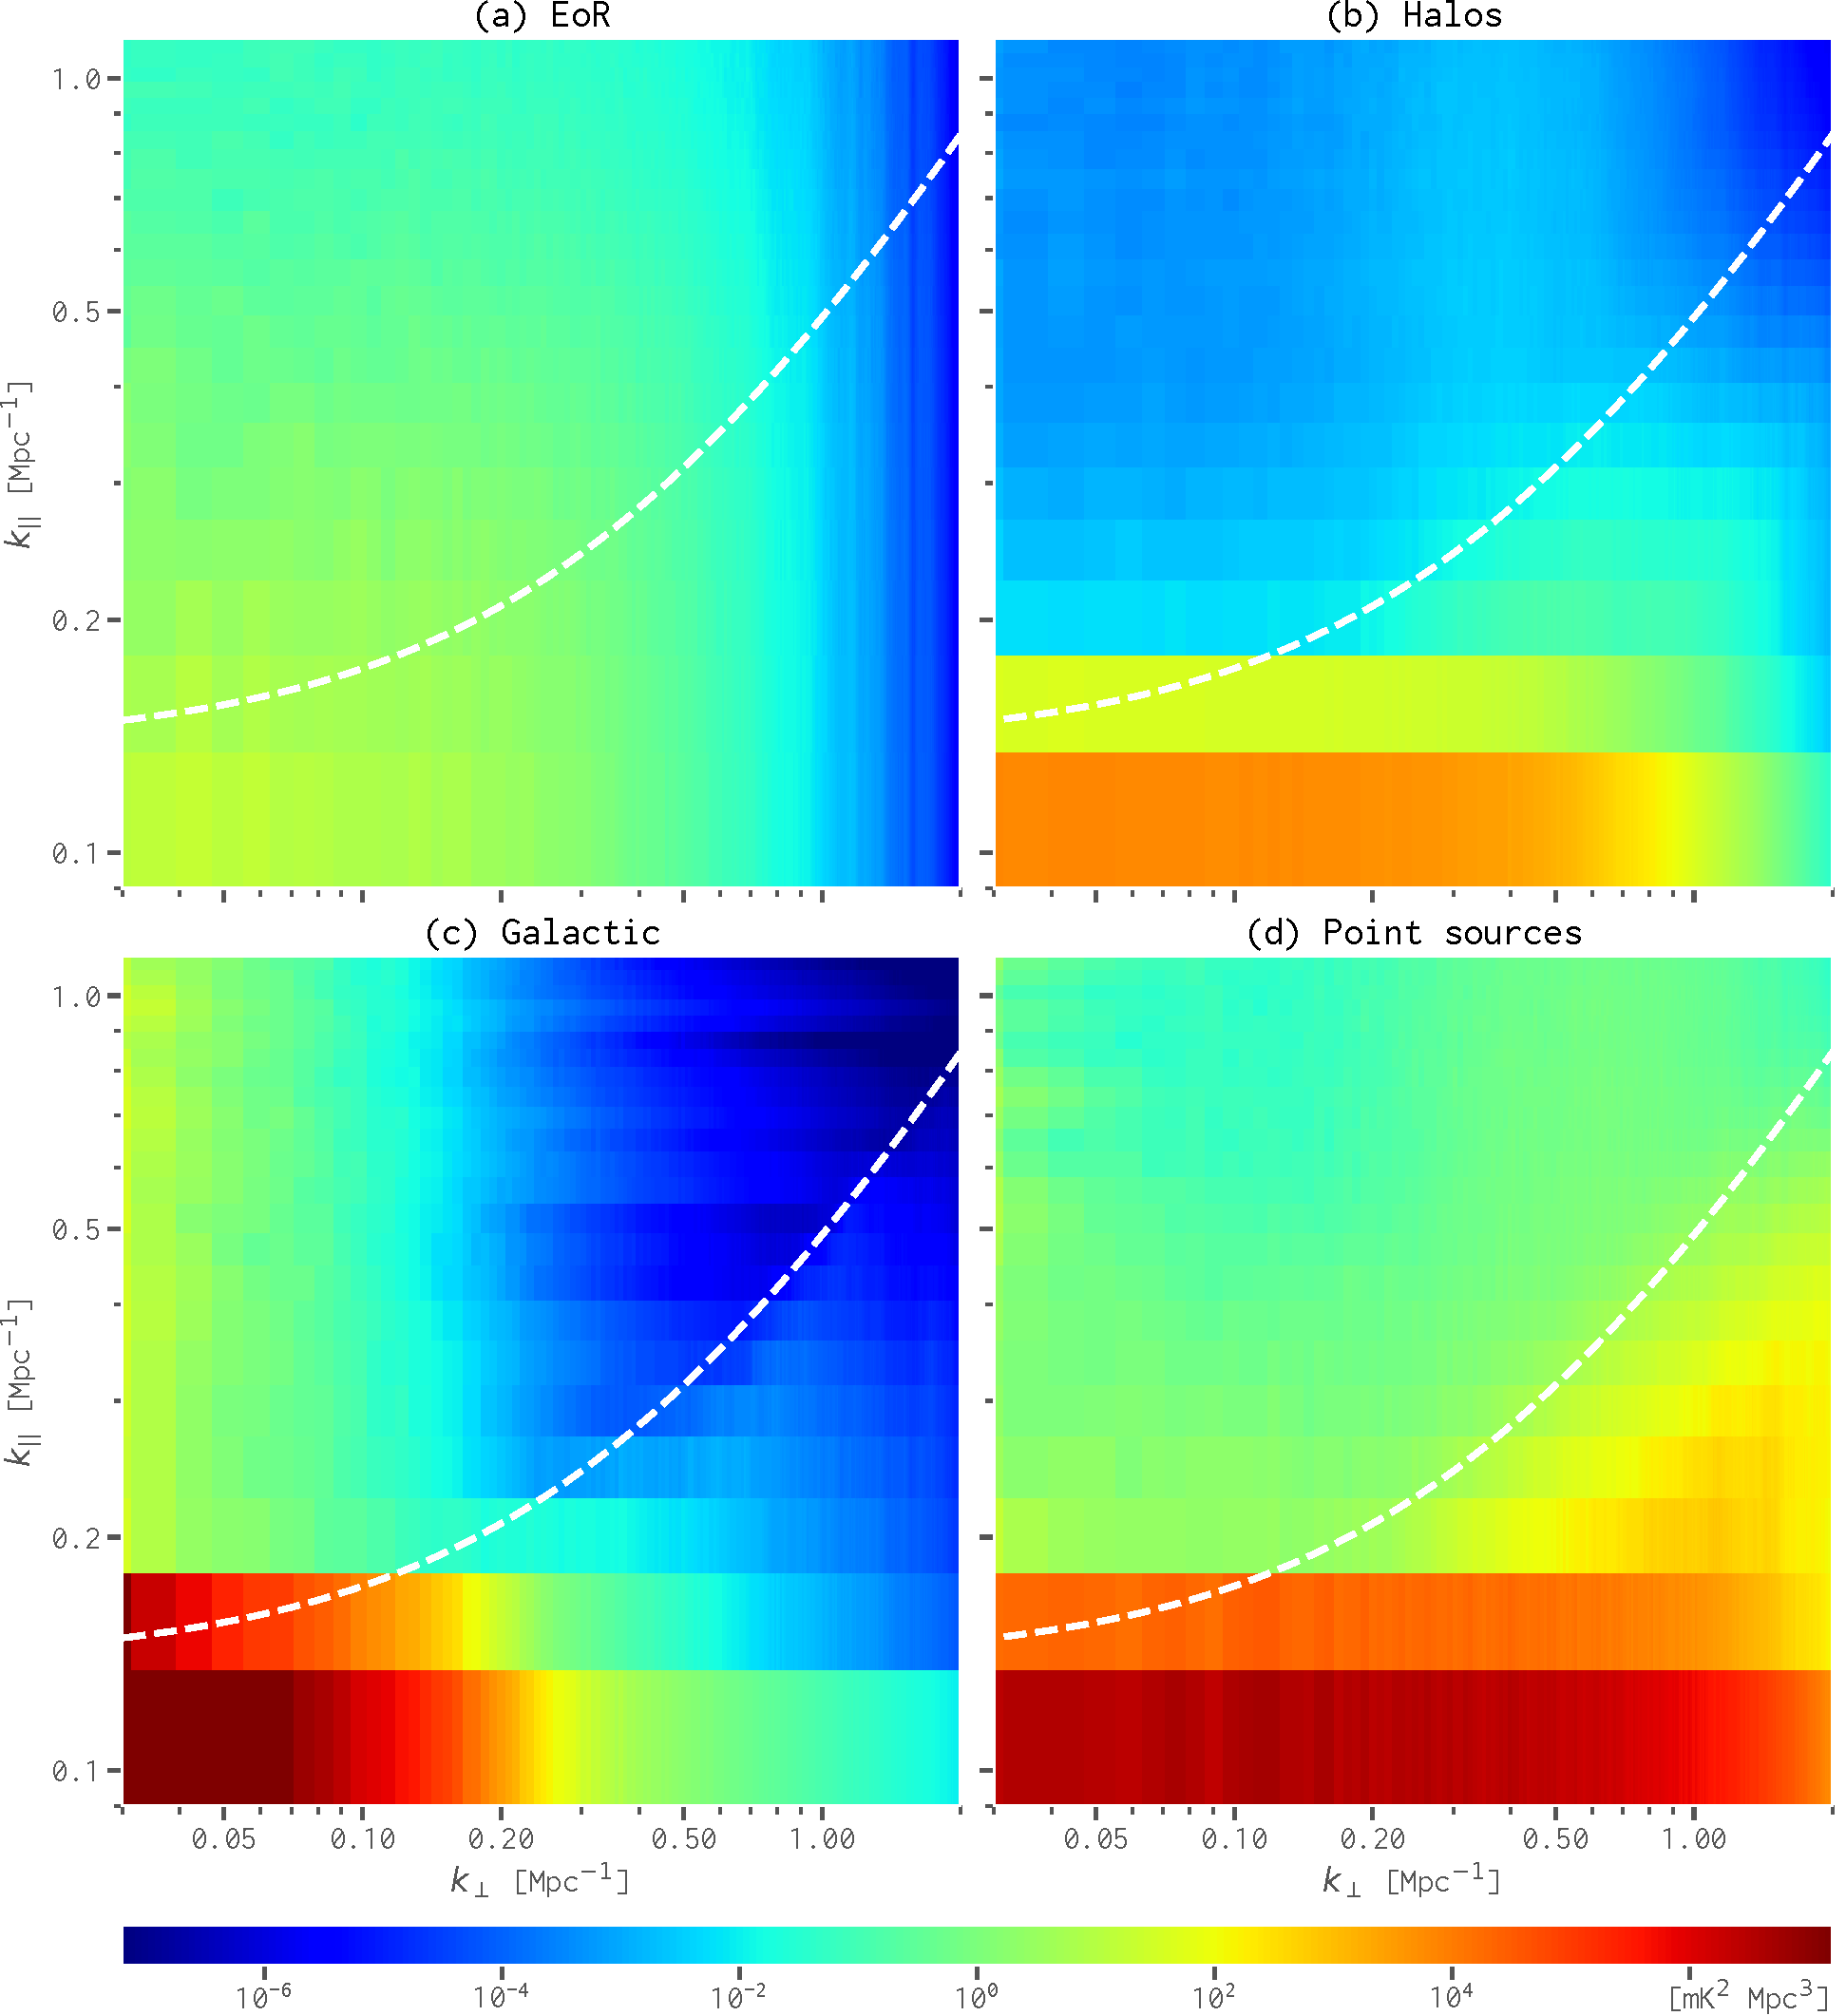
\includegraphics[height=0.95\textheight]{ps2d-band158}
    \end{figure}
  \end{alertblock}
\end{frame}

%............
\begin{frame}[subsec]
  \frametitle{EoR 窗口和前景楔形}
  仪器的色彩效应 $\rightarrow$
  $k_{\perp}$ 模式的功率混合到 $k_{\parallel}$ 模式里 $\rightarrow$
  前景楔形
  \begin{figure}
    \centering
    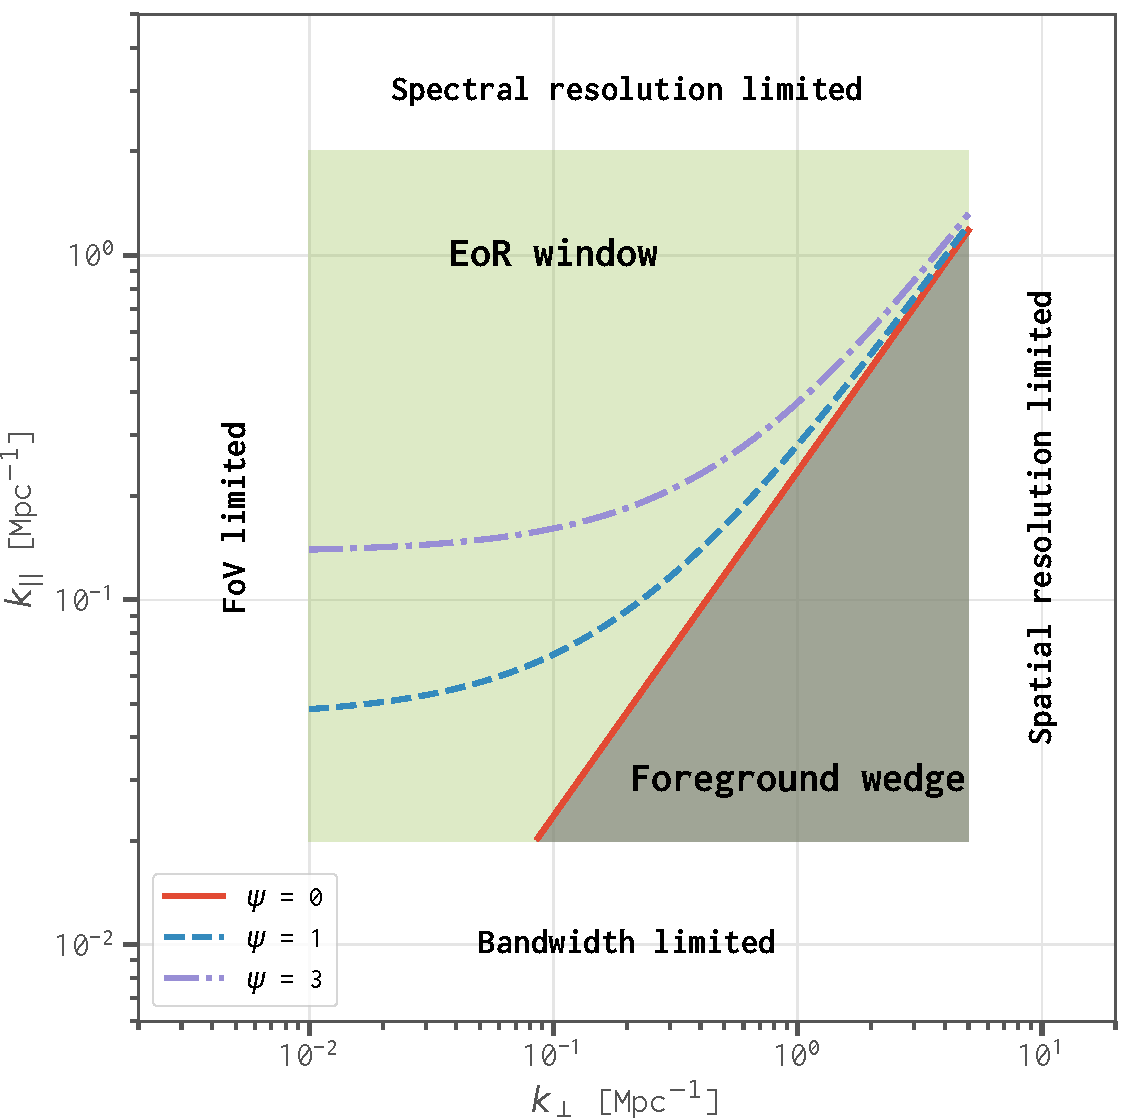
\includegraphics[height=0.8\textheight]{EoR-window}
  \end{figure}
\end{frame}

%---------------------------------------------------------------------
\subsection{一维功率谱的结果}

%............
\begin{frame}{3.2 一维功率谱的结果}
  \begin{figure}
    \centering
    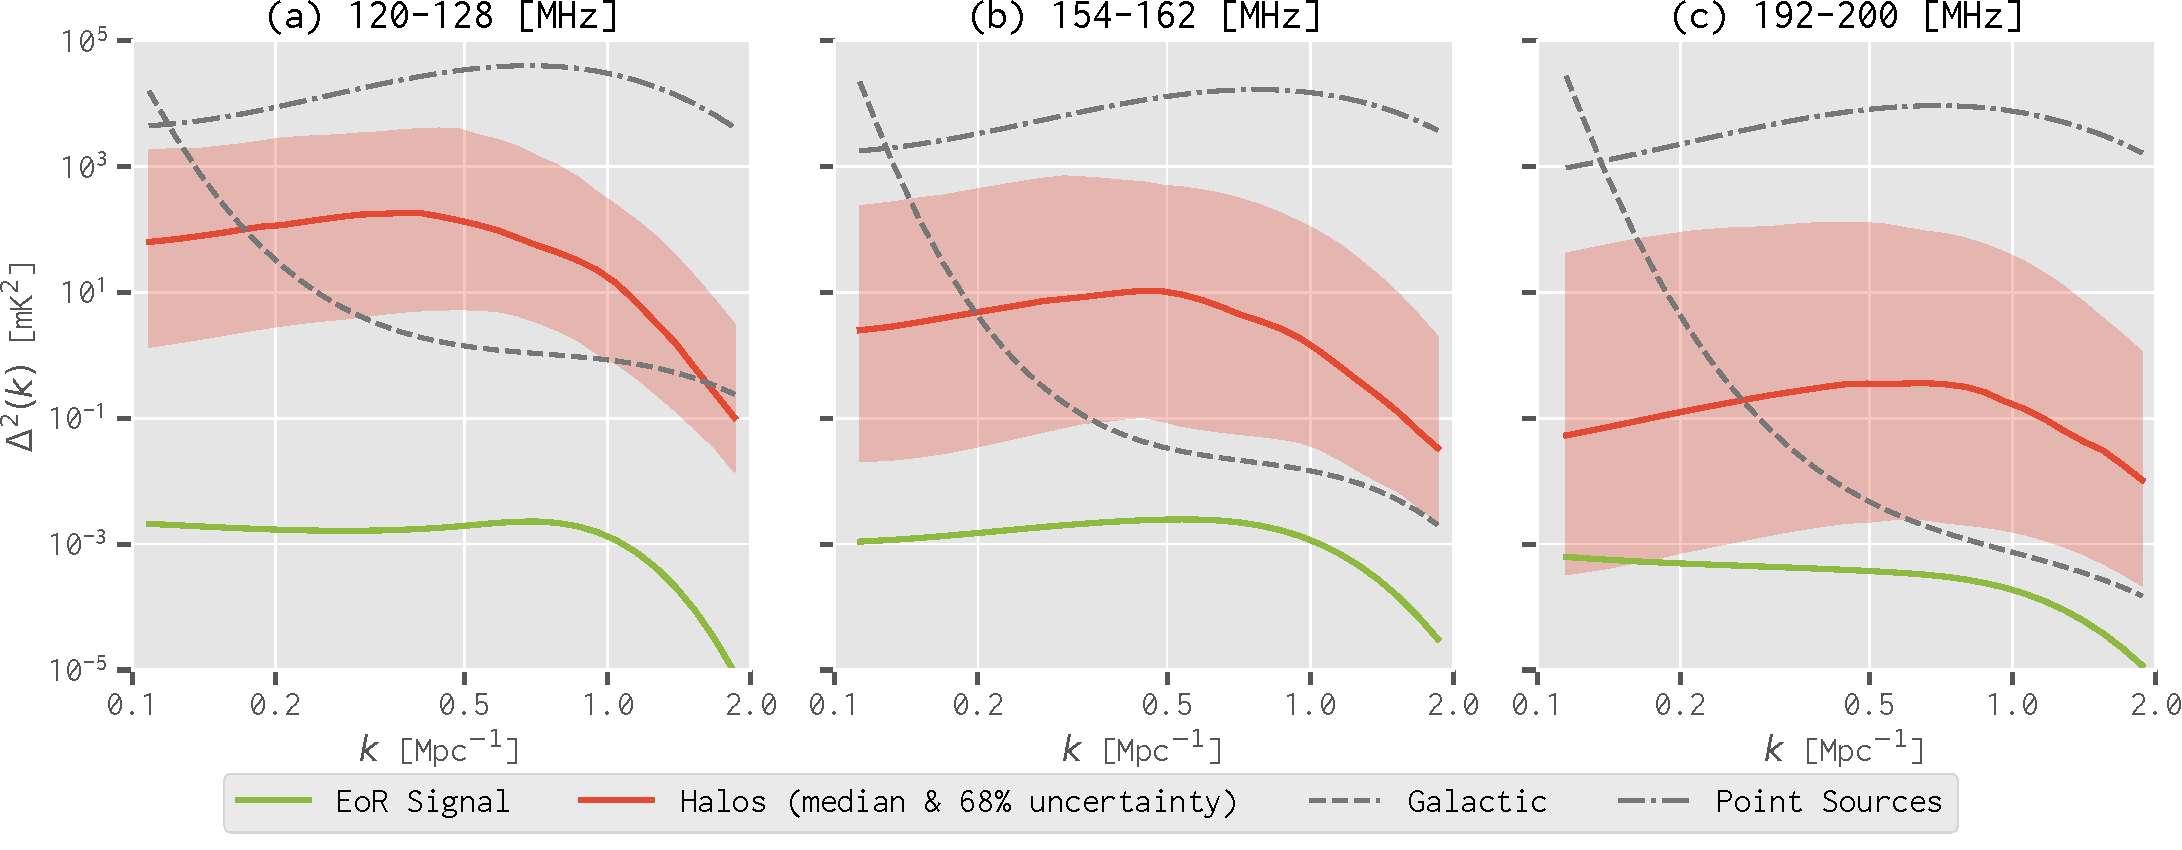
\includegraphics[width=\textwidth]{ps1d-3bands}
  \end{figure}
  \vspace{-1ex}
  尺度 \SI{1.2}{\arcminute}--\SI{24}{\arcminute}
  ($k \sim \SIrange{0.1}{2}{\per\Mpc}$):
  \vspace{-0.5ex}
  \begin{table}
    \centering
    \begin{tabular}{cc}
      \toprule
      频带 (\si{\MHz}) & $P_{\R{halo}} / P_{\R{eor}}$ \\
      \midrule
      120--128 & $\sim$\,\num{10000} \\
      154--162 & $\sim$\,1000 \\
      192--200 & $\sim$\,300 \\
      \bottomrule
    \end{tabular}
  \end{table}
\end{frame}

%---------------------------------------------------------------------
\subsection{二维功率谱的结果}

%............
\begin{frame}{3.3 二维功率谱的结果}
  \begin{figure}
    \centering
    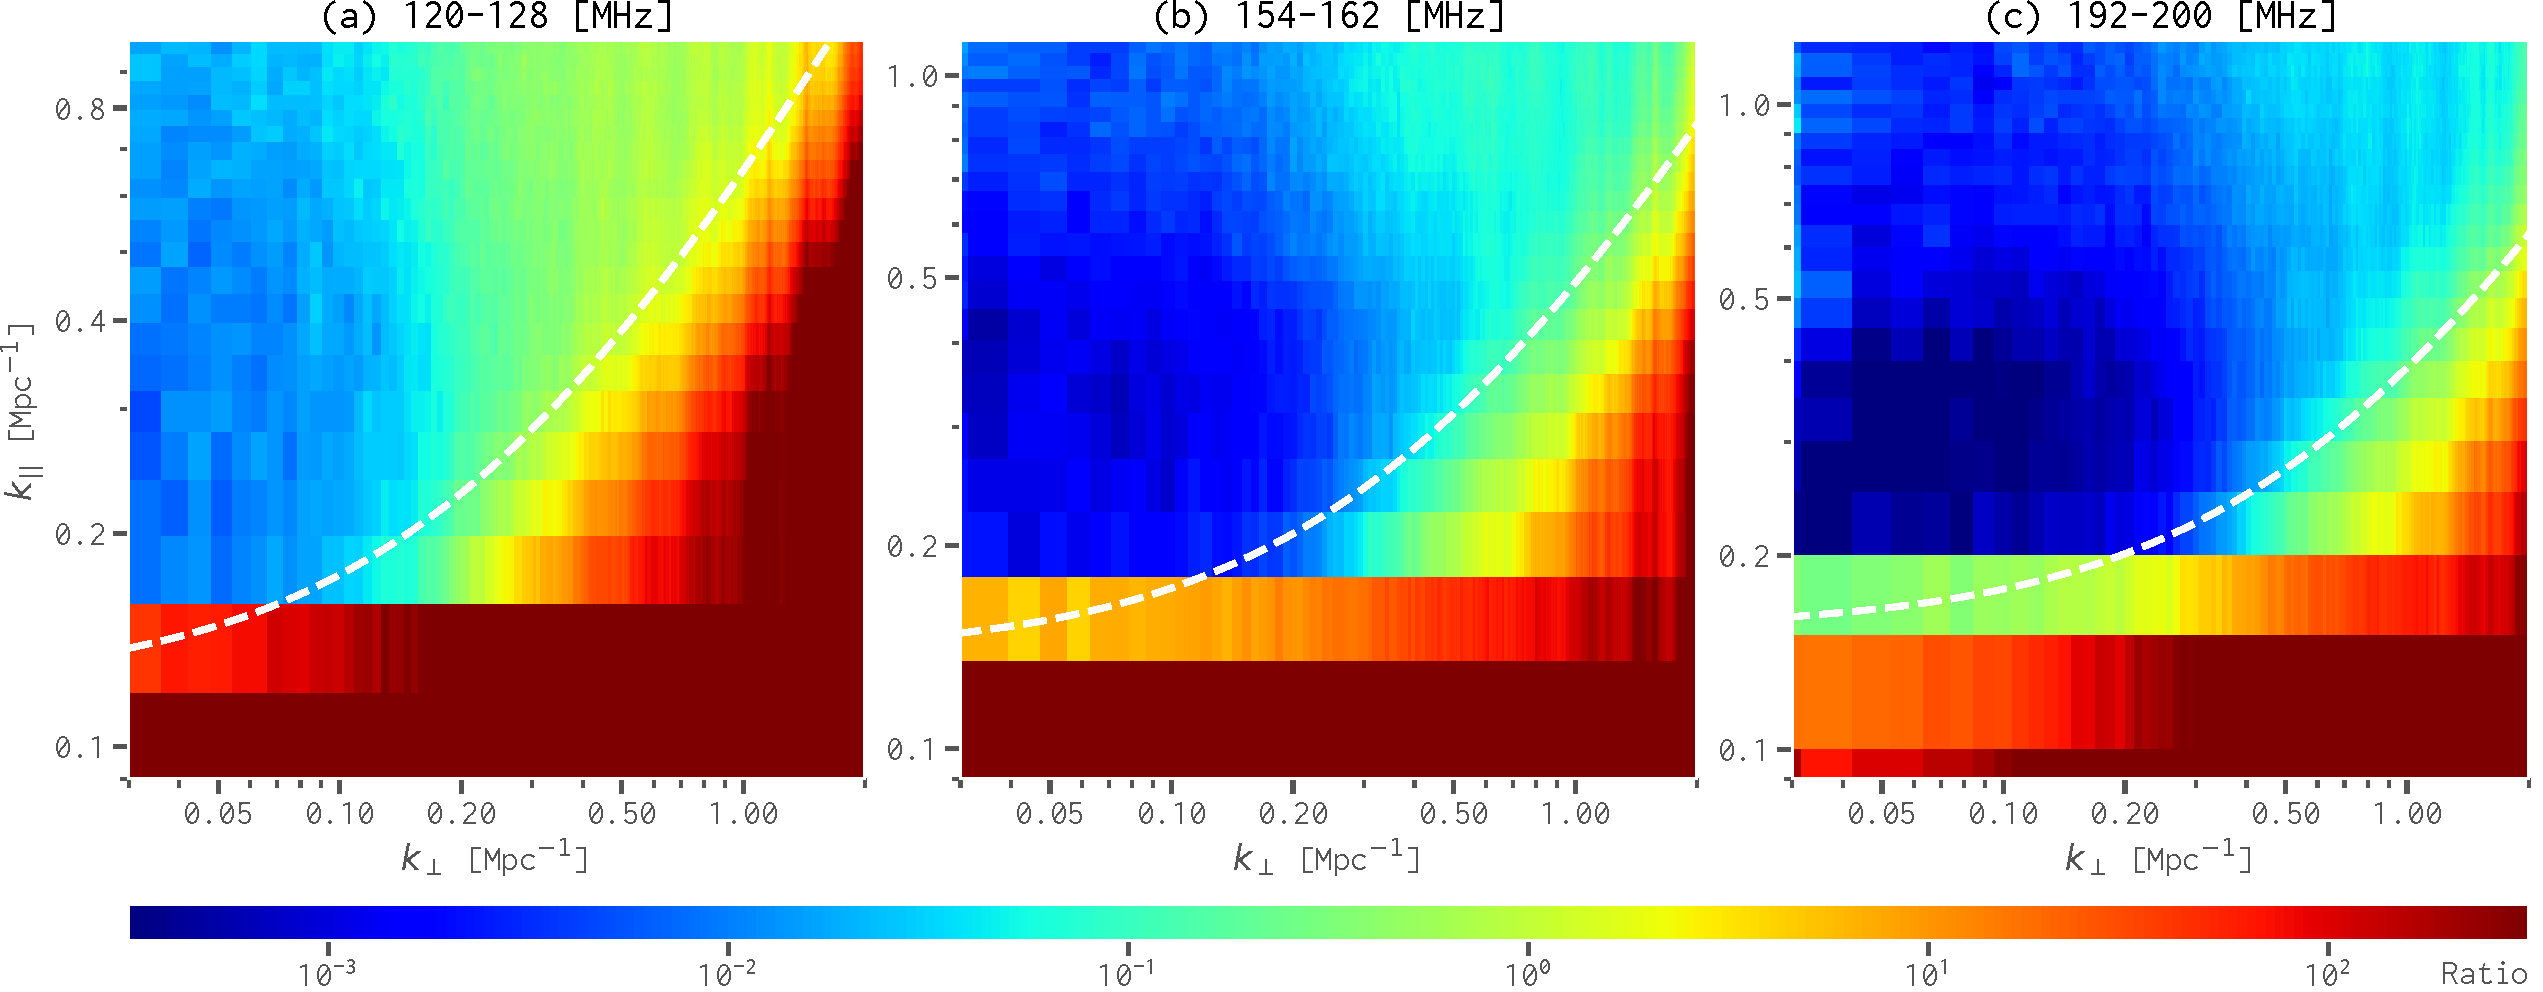
\includegraphics[width=\textwidth]{ps2d-ratio-3bands}
  \end{figure}
  \vspace{-1ex}
  射电晕辐射与 EoR 信号的\alert{二维功率谱之比}:
  \vspace{-0.5ex}
  \begin{table}
    \centering
    \begin{tabular}{cc}
      \toprule
      频带 (\si{\MHz}) & 污染尺度 \\
      \midrule
      120--128 & $k_{\perp} \gtrsim \SI{0.1}{\per\Mpc}$
                 ($\lesssim \SI{22}{\arcminute}$) \\
      154--162 & $k_{\perp} \gtrsim \SI{0.3}{\per\Mpc}$
                 ($\lesssim \SI{8}{\arcminute}$) \\
      192--200 & $k_{\perp} \gtrsim \SI{0.5}{\per\Mpc}$
                 ($\lesssim \SI{5}{\arcminute}$) \\
      \bottomrule
    \end{tabular}
  \end{table}
\end{frame}

%............
\begin{frame}[subsec]
  \frametitle{EoR 窗口内一维功率比的结果}
  \begin{columns}[t,onlytextwidth]
    \column{0.45\textwidth}
      尺度 \SI{2.4}{\arcminute}--\SI{4.8}{\arcminute}
      ($k \sim \SIrange{0.5}{1}{\per\Mpc}$):
      \vspace{-1ex}
      \begin{table}
        \small
        \begin{tabular}{cc}
          \toprule
          频带 (\si{\MHz}) & $\max(P_{\R{halo}} / P_{\R{eor}})$ \\
          \midrule
          120--128 & $\sim$\,230--800\% \\
          154--162 & $\sim$\,18--95\% \\
          192--200 & $\sim$\,7-40\% \\
          \bottomrule
        \end{tabular}
      \end{table}
      EoR 窗口内的射电晕辐射仍然不可忽略

    \column{0.53\textwidth}
    \begin{figure}
      \centering
      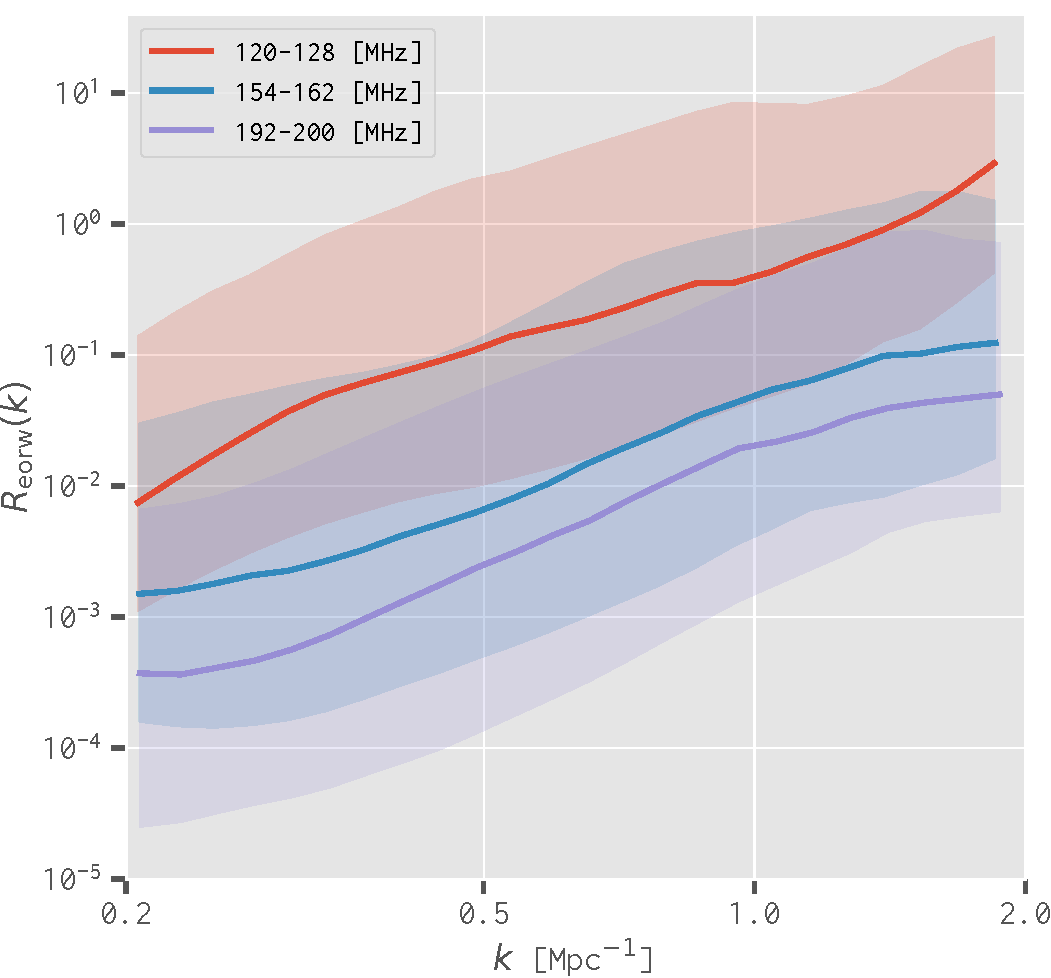
\includegraphics[width=\columnwidth]{ps1d-ratio-3bands}
    \end{figure}
  \end{columns}
\end{frame}

%---------------------------------------------------------------------
\subsection{频谱伪结构对射电晕辐射的影响}

%............
\begin{frame}{3.4 频谱伪结构对射电晕辐射的影响}
  \begin{itemize}
    \item 干涉阵列的频率响应约有 0.1--1\% 的校准不确定度
    \item \alert{频谱伪结构}幅度 $A_{\R{arti}} = 0.1\%$:
      射电晕辐射在 EoR 窗口内部分尺度的功率分别增加约 17、15、13 倍
    \item $A_{\R{arti}} = 1\%$:功率分别增加约 1700、1500、1300 倍
  \end{itemize}
  \vspace{-1ex}
  \begin{figure}
    \centering
    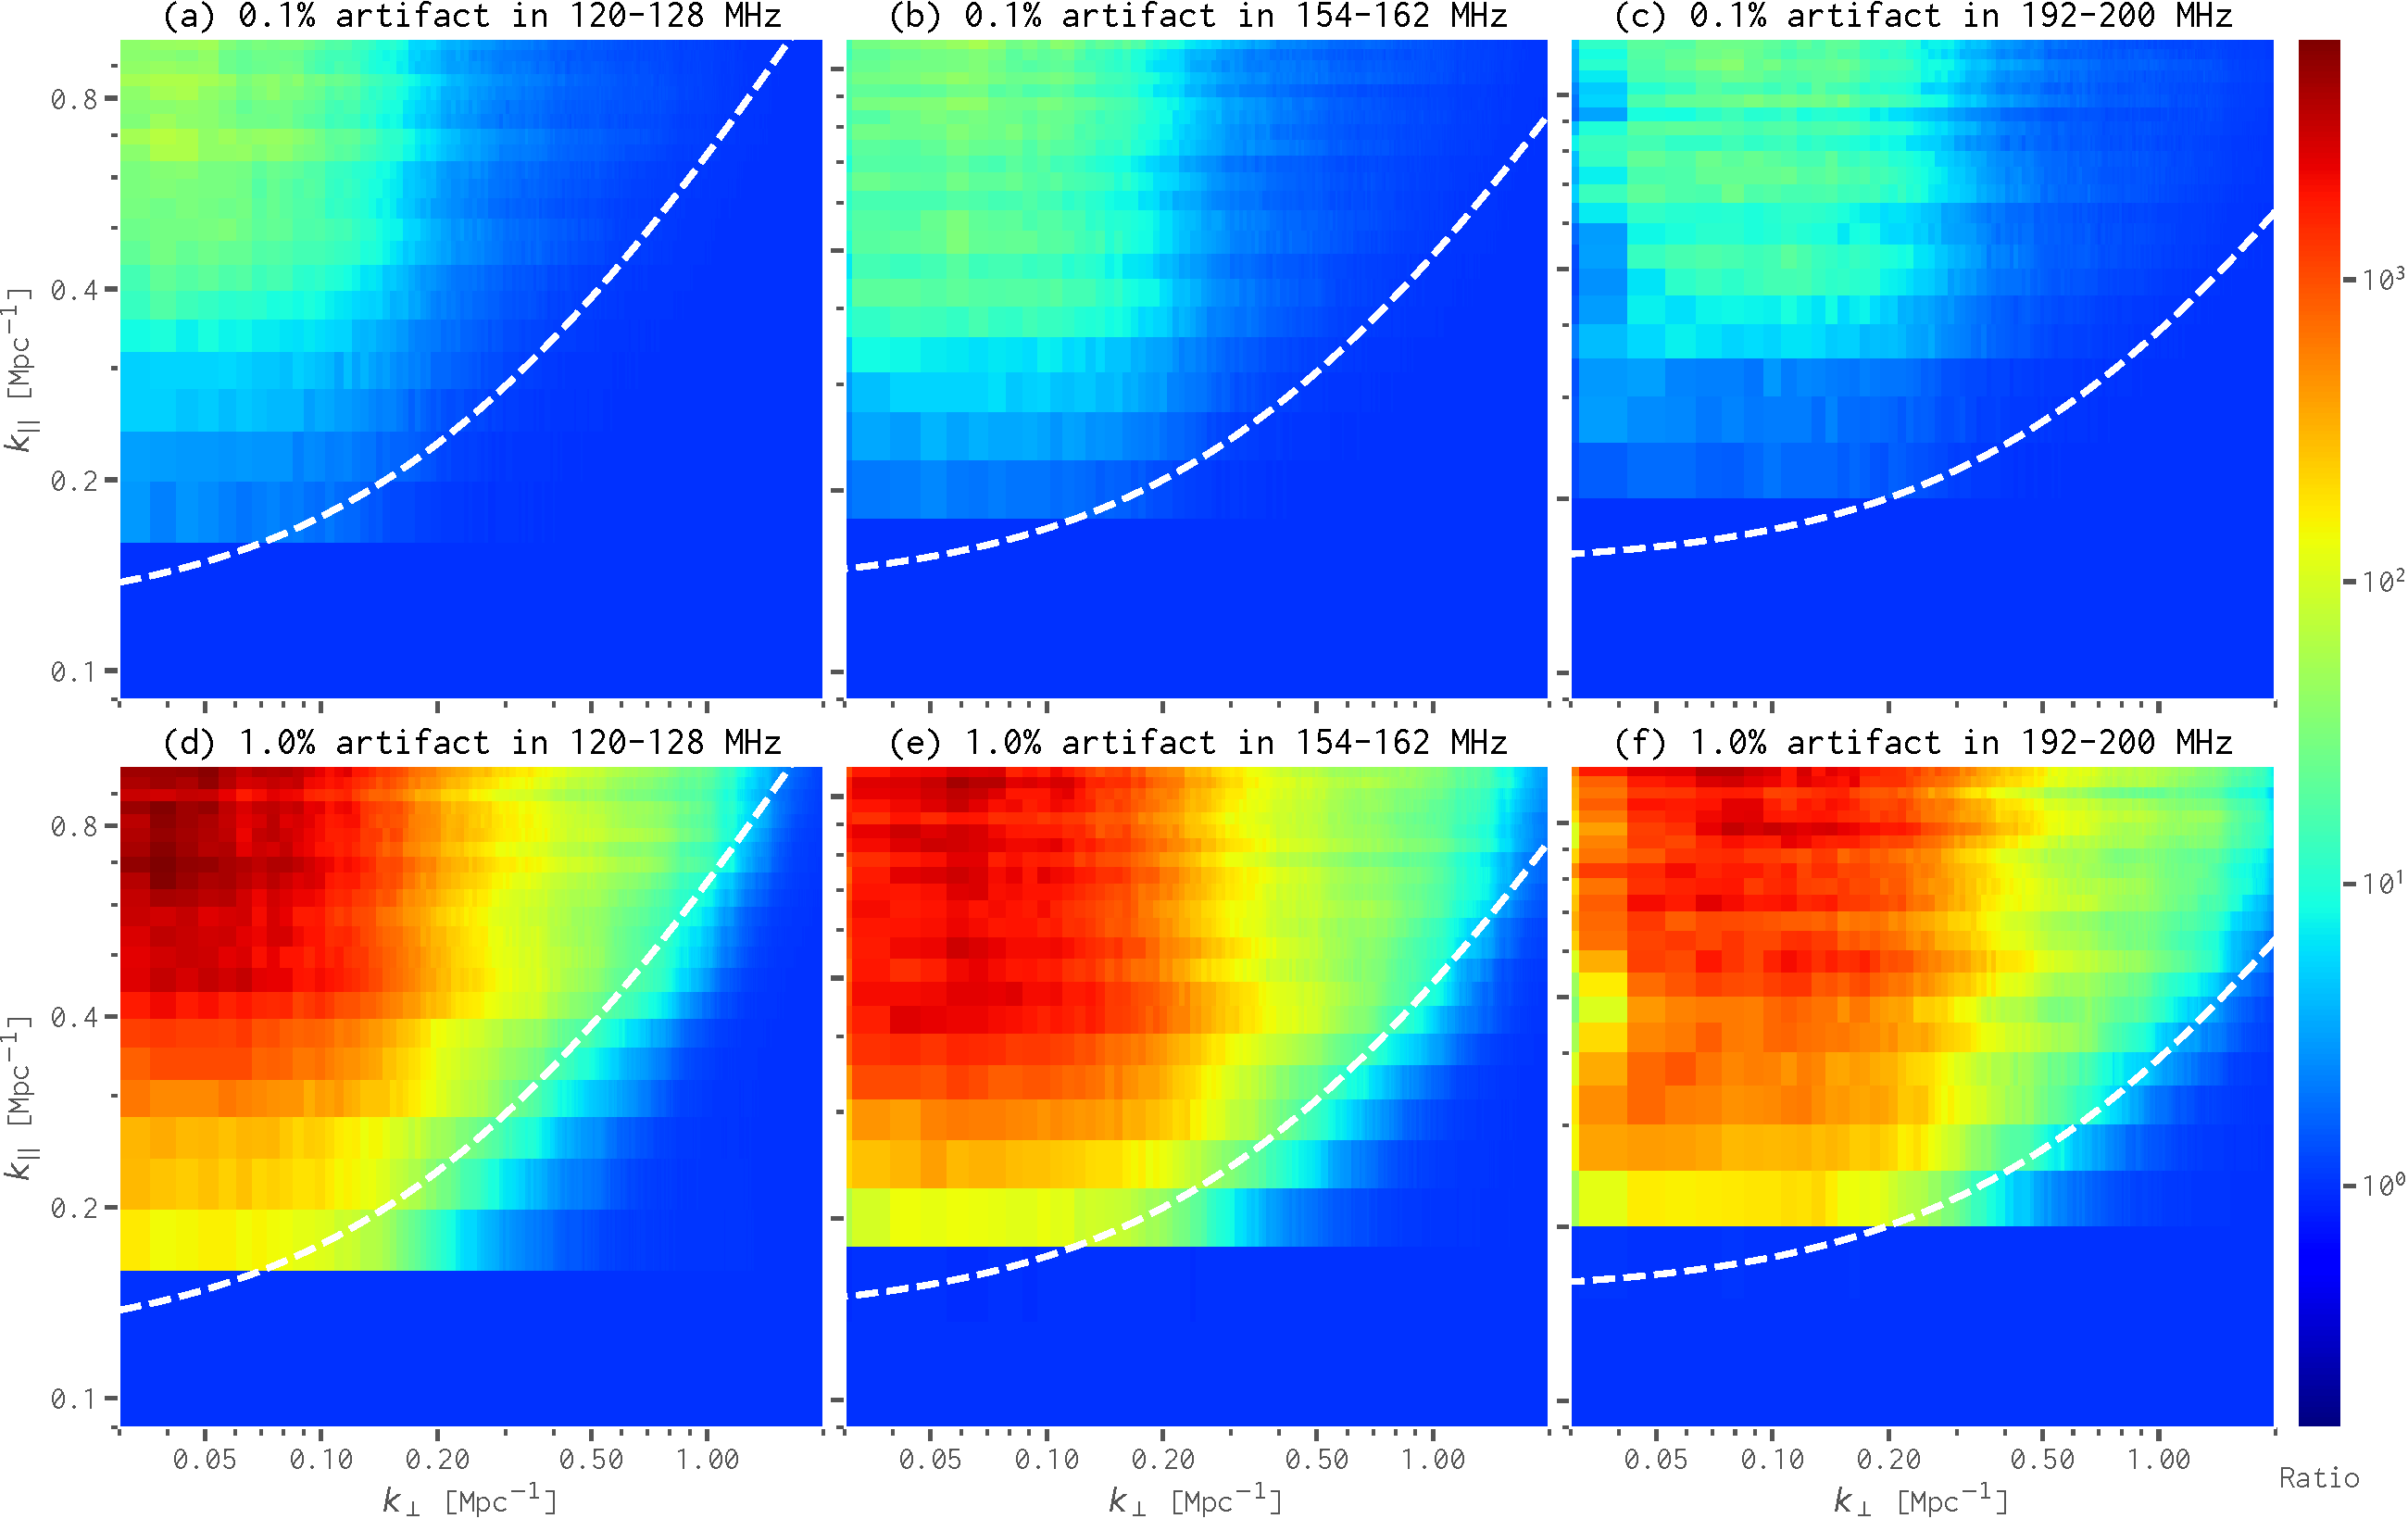
\includegraphics[height=0.7\textheight]{ps2d-ratio-crp-3bands}
  \end{figure}
\end{frame}

%---------------------------------------------------------------------
\subsection{旁瓣内射电晕辐射对 EoR 探测的影响}

%............
\begin{frame}{3.5 旁瓣内射电晕辐射对 EoR 探测的影响}
  \begin{itemize}
    \item \alert{远旁瓣致淆噪声 (FSCN)}:场外源通过旁瓣在视场中产生干扰
    \item 模拟新射电晕图像:从角半径 \SI{10}{\degree} 覆盖至地平线
    \item 射电晕 FSCN 在 EoR 窗口内的功率可达 EoR 信号约 20 倍
  \end{itemize}
  \vspace{-1ex}
  \begin{figure}
    \centering
    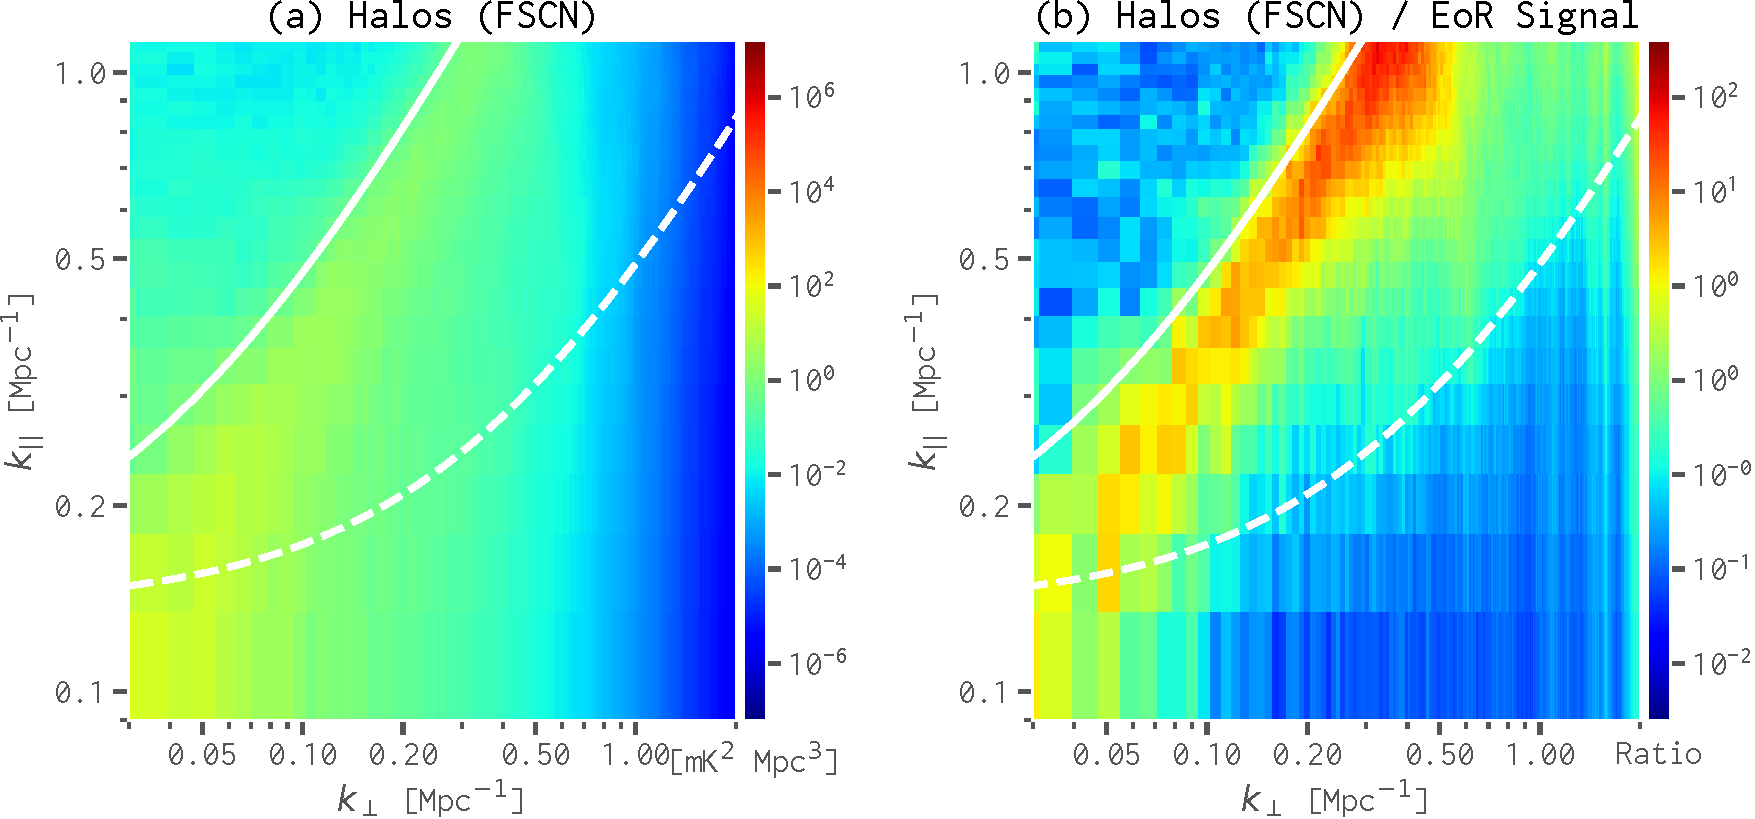
\includegraphics[width=\textwidth]{ps2d-fscn}
  \end{figure}
\end{frame}


%=====================================================================
\section{基于深度学习的 EoR 信号分离算法}

\begin{frame}
  \begin{block}{本节提纲}
    \vspace{2ex}
    \tableofcontents[
      sections=\value{section},
      sectionstyle=hide,
    ]
  \end{block}
\end{frame}

%---------------------------------------------------------------------
\subsection{EoR 信号分离原则}

%............
\begin{frame}{4.1 EoR 信号分离原则}
  \begin{itemize}
    \item EoR 信号沿频率方法剧烈变化
    \item 前景辐射的频谱在本质上非常光滑
    \item 利用两者的频谱结构差异实现 EoR 信号的分离
  \end{itemize}
\end{frame}

\begin{frame}[subsec]
  \frametitle{波束效应对频谱光滑性的影响}
  \begin{columns}[t,onlytextwidth]
    \column{0.48\textwidth}
    \begin{itemize}
      \item 旁瓣位置随频率增大而向中间移动 ($\theta \propto 1/\nu$)
      \item 干扰源的辐射分布随频率变化
      \item 考虑视场中一个位置,频率维度出现小尺度涨落
      \item 前景辐射的频谱光滑性受损,传统前景扣除方法失效
    \end{itemize}

    \column{0.5\textwidth}
    \begin{figure}
      \centering
      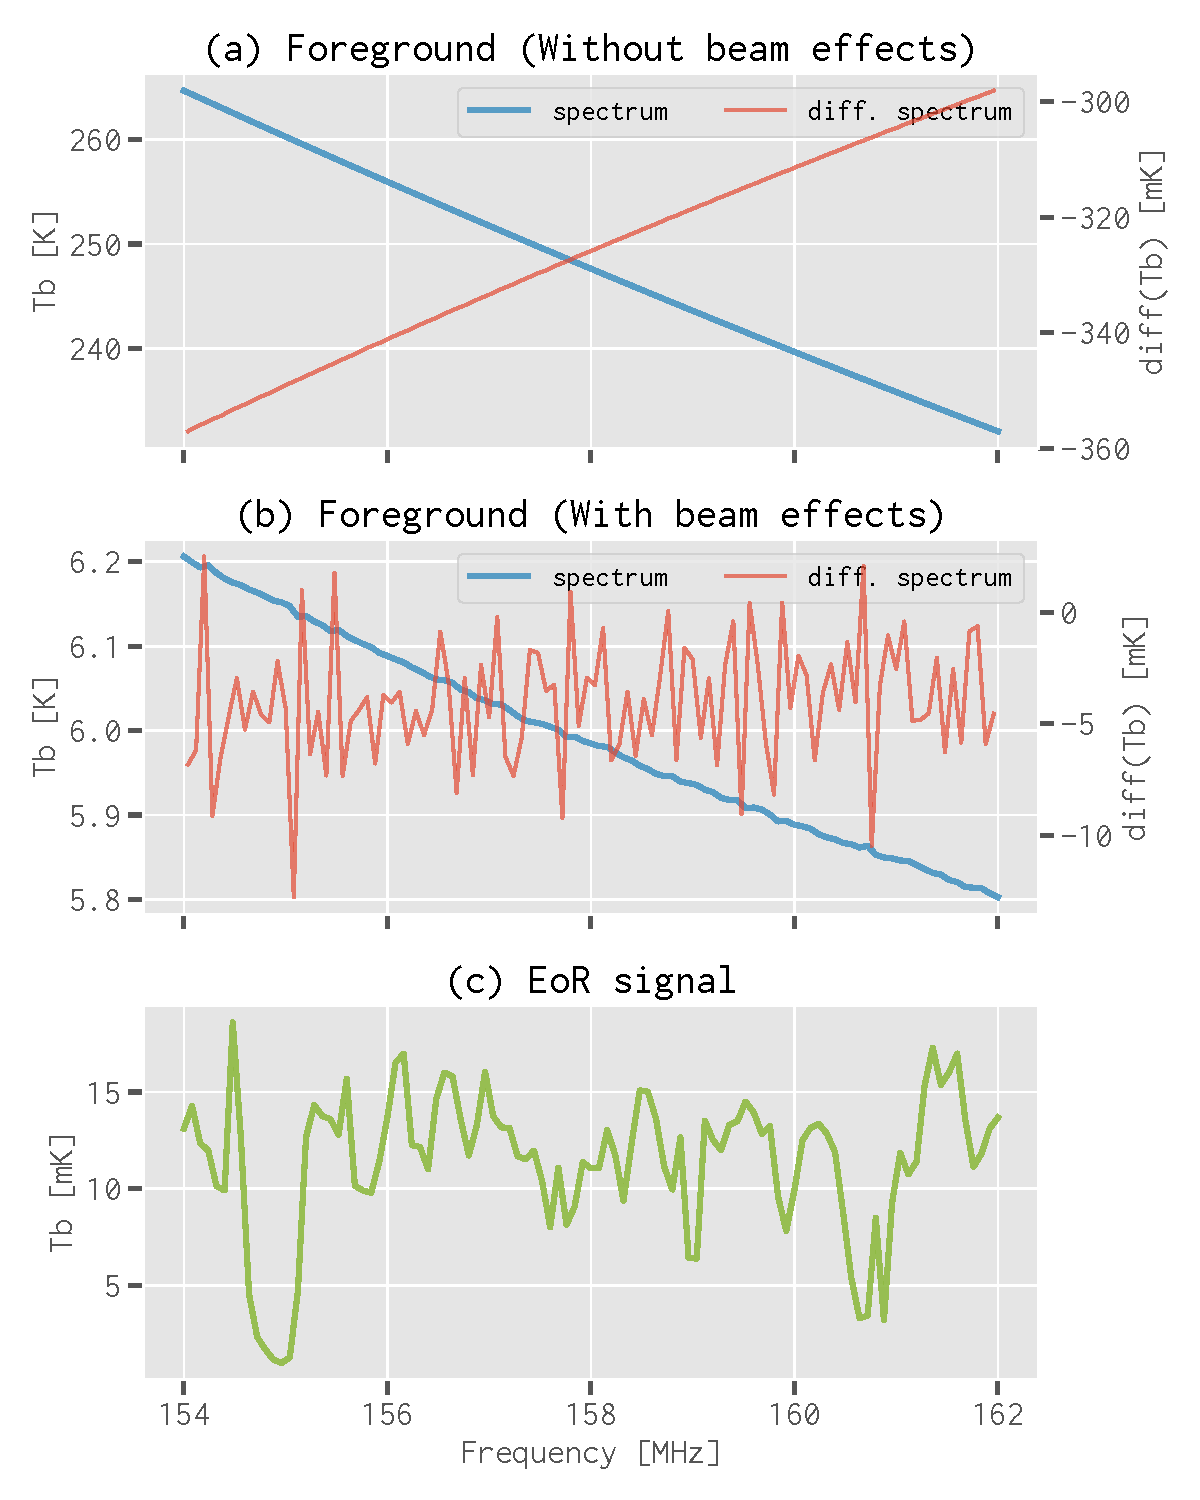
\includegraphics[width=\columnwidth]{cdae-simdata-example}
    \end{figure}
  \end{columns}
\end{frame}

%---------------------------------------------------------------------
\subsection{基于深度学习的新算法}

%............
\begin{frame}{4.2 基于深度学习的新算法}
  \begin{figure}
    \centering
    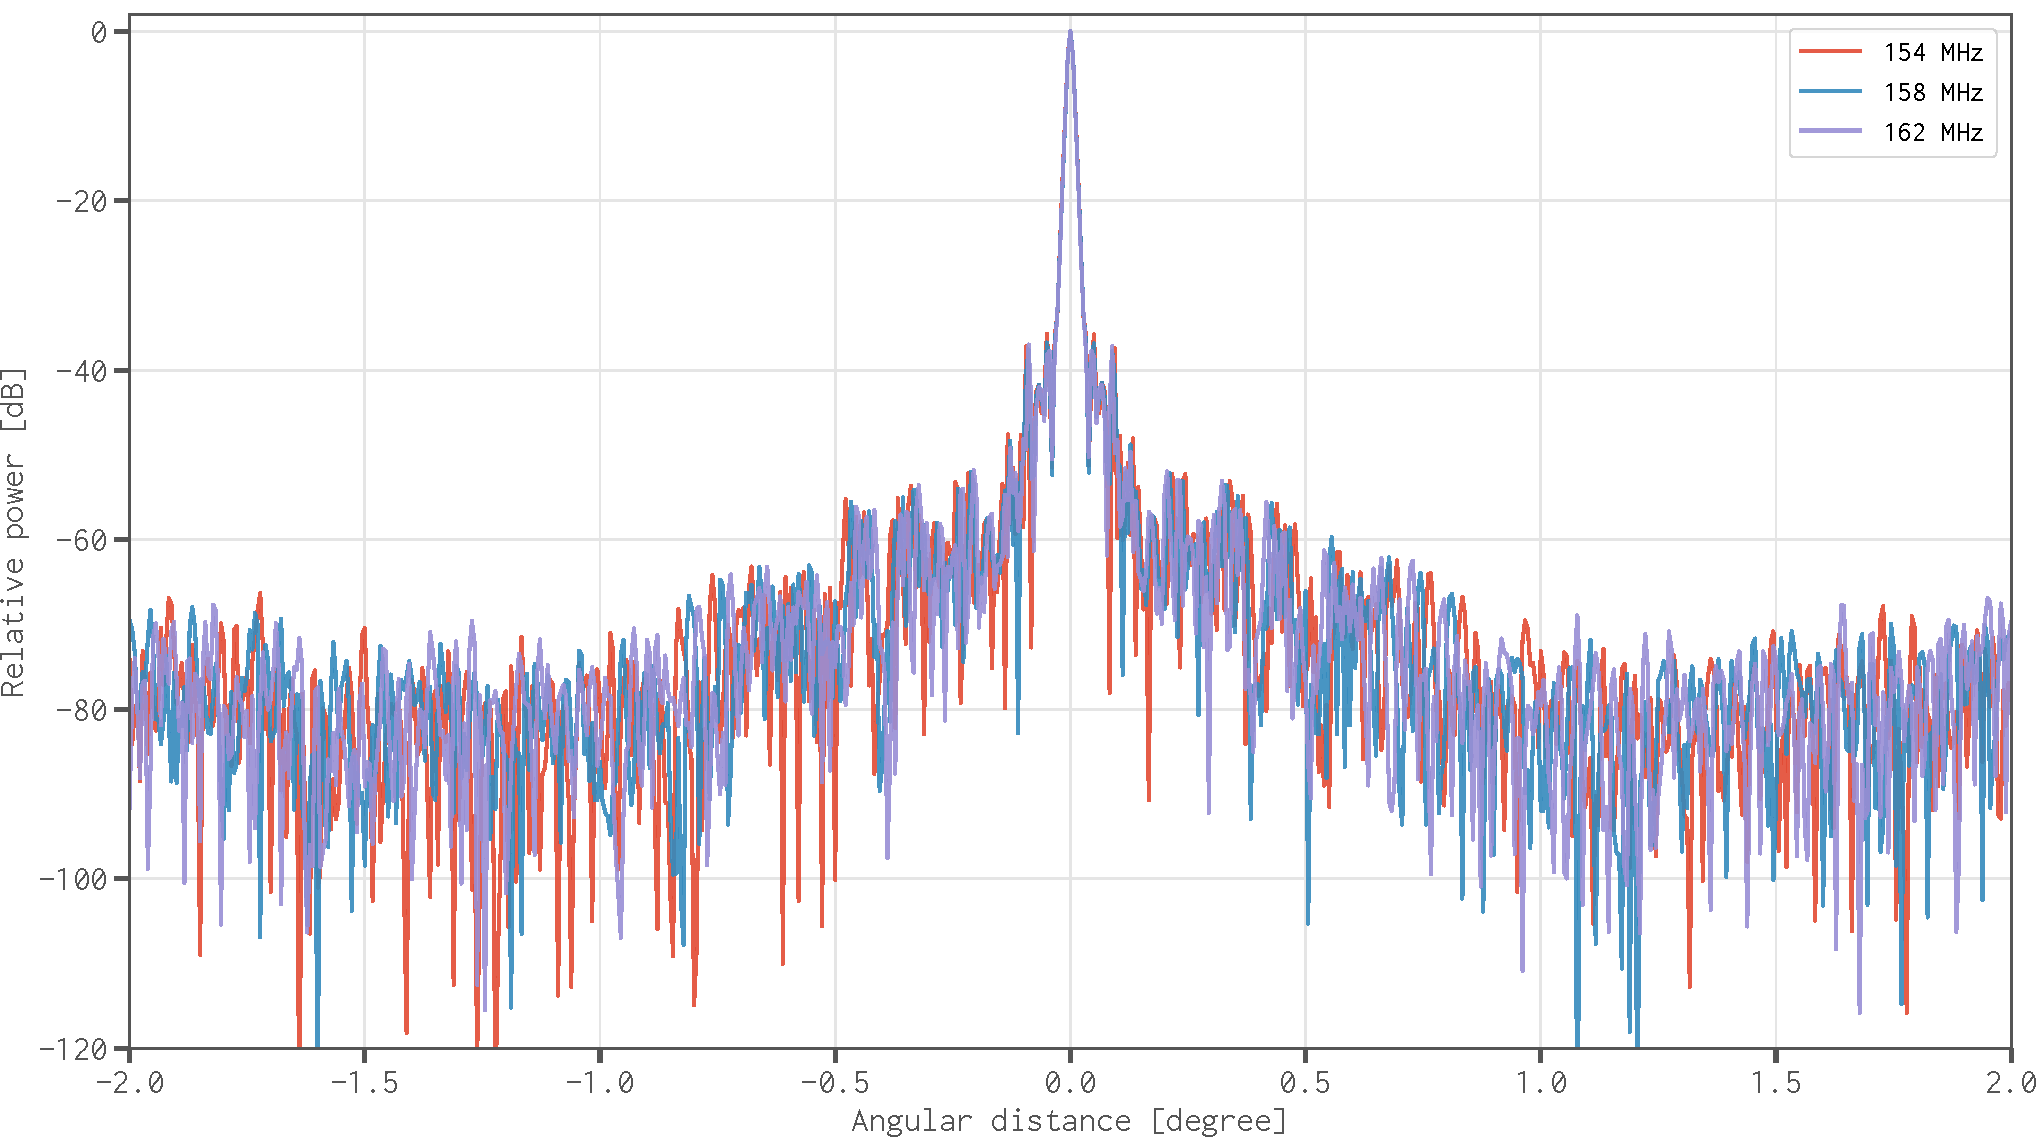
\includegraphics[height=0.54\textheight]{SKA1-low-psf}
  \end{figure}

  \begin{itemize}
    \item 对波束效应进行解析建模几乎不可行
    \item \alert{深度学习}是一条可能的途径:
      \begin{itemize}
        \item 从数据中学习特征并自适应地优化模型
        \item 一旦训练好,使用过程非常高效
        \item 灵活性高,易扩展用于其他望远镜
      \end{itemize}
  \end{itemize}
\end{frame}

%............
\begin{frame}[subsec]
  \frametitle{为什么采用 CDAE ?}
  \begin{itemize}
    \item EoR 信号分离问题可转化为 EoR 信号的\alert{去噪问题}
    \item EoR 信号为需要的信号,前景辐射为强烈的噪声
    \item \alert{自编码器}:深度学习算法中最常用的数据去噪算法之一
    \item \alert{卷积去噪自编码器 (CDAE)}: \\
      自编码器的去噪能力 + 卷积神经网络的特征提取能力 \\
      $\rightarrow$ 值得尝试
  \end{itemize}
\end{frame}

%............
\begin{frame}[subsec]
  \frametitle{CDAE 是什么?}
  \begin{figure}
    \centering
    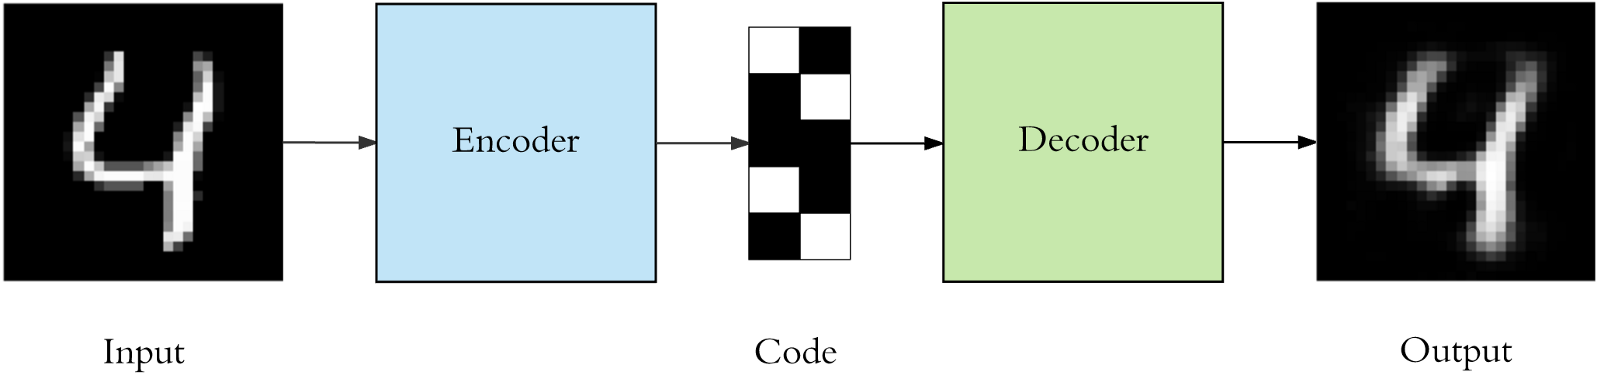
\includegraphics[width=0.7\textwidth]{autoencoder}
  \end{figure}
  \vspace{-0.8ex}
  \begin{alertblock}{自编码器}
    \vspace{-0.5ex}
    \begin{itemize}
      \item 由编码器 $f$ 和解码器 $g$ 组成:
        $\B{x} \rightarrow \B{h} = f(\B{x}) \rightarrow \B{r} = g(\B{h})$
      \item 训练使得重建信号 $\B{r}$ 的损失 $L(\B{r}, \B{x})$ 最小
    \end{itemize}
  \end{alertblock}
  \vspace{-0.3ex}
  \begin{alertblock}{去噪自编码器}
    \vspace{-0.5ex}
    \begin{itemize}
      \item 去噪训练策略:
        人为损坏 $\B{x}$ $\rightarrow$
        训练 $\rightarrow$ 使 $\B{r}$ 恢复 $\B{x}$
      \item 迫使学习一个更有效的表示,提升性能
    \end{itemize}
  \end{alertblock}
  \vspace{-0.3ex}
  \begin{alertblock}{卷积去噪自编码器}
    \vspace{-0.5ex}
    \begin{itemize}
      \item 使用卷积层的去噪自编码器
      \item 拥有更强的特征提取能力,提升去噪能力
    \end{itemize}
  \end{alertblock}
\end{frame}

%............
\begin{frame}[subsec]
  \frametitle{CDAE 网络架构}
  \begin{itemize}
    \item 编码器:4 层 (32, 64, 64, 32)
    \item 解码器:5 层 (32, 64, 64, 32, 1)
    \item 过滤器尺寸:3
    \item 输出层:\alert{tanh} 激活函数
    \item 其余层:\alert{指数线性单元} (ELU),\alert{批标准化} (BN)
  \end{itemize}

  \begin{figure}
    \makebox[\textwidth][c]{%
      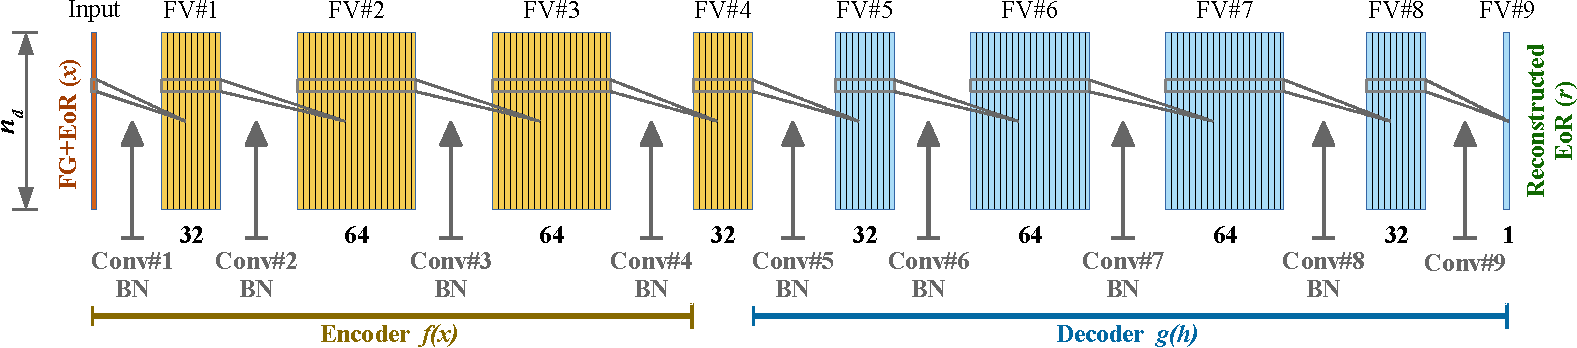
\includegraphics[width=1.1\textwidth]{cdae-network-crop}}
  \end{figure}
\end{frame}

%............
\begin{frame}[subsec]
  \frametitle{训练和评估方法}
  \begin{itemize}
    \item 三个数据集:
      \begin{itemize}
        \item \alert{训练集 $S_{\R{tr}}$}:拟合待训练参数
        \item \alert{验证集 $S_{\R{val}}$}:验证训练过程是否正常;约束超参数
        \item \alert{测试集 $S_{\R{test}}$}:训练结束后用于评估性能
      \end{itemize}
    \item 损失 $L(\B{r}, \B{x})$ 由\alert{均方误差}量化:
      \begin{equation}
        L = \frac{1}{N_{\R{tr}}} \sum_{i=1}^{N_{\R{tr}}}
            \left[ \B{r}_{\R{eor}}^{(i)} - \B{x}_{\R{eor}}^{(i)} \right]^T
            \left[ \B{r}_{\R{eor}}^{(i)} - \B{x}_{\R{eor}}^{(i)} \right]
      \end{equation}
    \item 评估指标采用\alert{相关系数}:
      \begin{equation}
        \xi(\B{r}_{\R{eor}}, \B{x}_{\R{eor}})
          = \frac{\sum_{j=1}^{n}(r_{\R{eor},j} - \bar{r}_{\R{eor}})
              (x_{\R{eor},j} - \bar{x}_{\R{eor}})}{
                \sqrt{\sum_{j=1}^{n}(r_{\R{eor},j} - \bar{r}_{\R{eor}})^2
                \sum_{j=1}^{n}(x_{\R{eor},j} - \bar{x}_{\R{eor}})^2}
            }
      \end{equation}
  \end{itemize}
\end{frame}

%---------------------------------------------------------------------
\subsection{新算法的演示}

%............
\begin{frame}{4.3 新算法的演示}
  \begin{alertblock}{主要流程}
    \begin{enumerate}
      \item 模拟训练数据
      \item 预处理数据
      \item 训练 CDAE
      \item 测试 CDAE 的分离效果
      \item 对比传统前景扣除算法
    \end{enumerate}
  \end{alertblock}
\end{frame}

%............
\begin{frame}[subsec]
  \frametitle{训练数据的模拟和预处理}
  \begin{itemize}
    \item 模拟两组 SKA 图像立方:
      EoR 信号 $C_{\R{eor}}$,前景辐射 $C_{\R{fg}}$
      \begin{itemize}
        \item \SIrange{154}{162}{\MHz},频率分辨率 \SI{80}{\kHz},
          尺寸 \num{360 x 360 x 101}
        \item 形成数据集 $S = \left\{ \left(\B{x}^{(i)},
          \,\B{x}^{(i)}_{\R{eor}} \right) \right\}$,
          其中 $\B{x}^{(i)} = \B{x}^{(i)}_{\R{eor}} + \B{x}^{(i)}_{\R{fg}}$
      \end{itemize}
    \item 预处理输入数据 $X = \big\{ \B{x}^{(i)} \big\}$
      和输入 EoR 信号 $X_{\R{eor}} = \big\{ \B{x}^{(i)}_{\R{eor}} \big\}$
    \item 划分为三个数据集:
      \begin{itemize}
        \item 第一组:80\% 为训练集 $S_{\R{tr}}$,20\% 为验证集 $S_{\R{val}}$
        \item 第二组:全部为测试集 $S_{\R{test}}$
      \end{itemize}
  \end{itemize}
\end{frame}

%............
\begin{frame}[subsec]
  \frametitle{CDAE 的训练结果}
  \begin{figure}
    \centering
    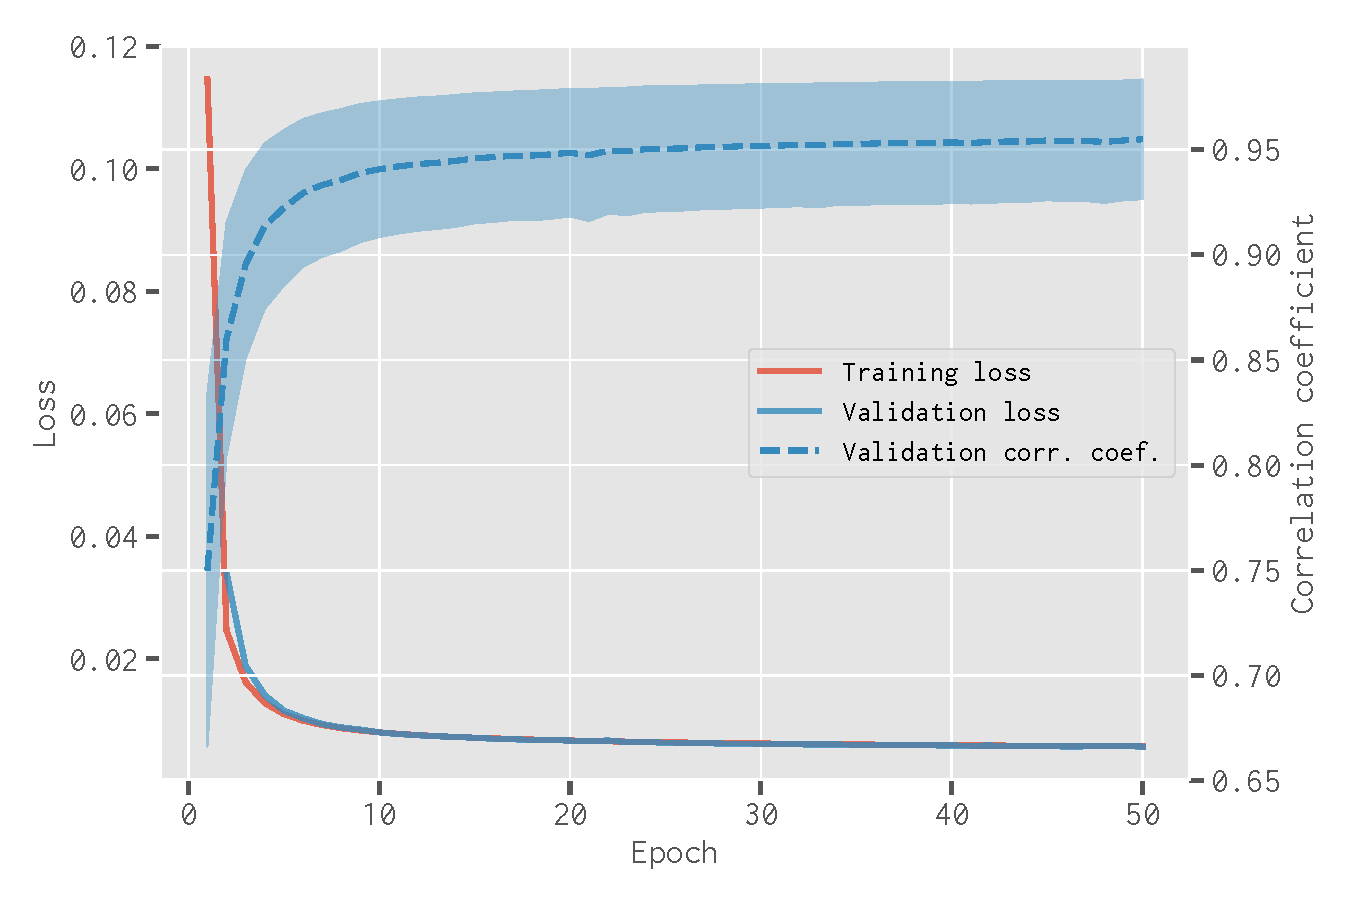
\includegraphics[width=0.8\textwidth]{cdae-train}
  \end{figure}
  \vspace{-1ex}
  训练损失 $L_{\R{tr}}$ 和验证损失 $L_{\R{val}}$ 平稳减小,
  评估指标 $\xi$ 稳步上升 \\
  $\rightarrow$
  训练效果良好,无过拟合
\end{frame}

%............
\begin{frame}[subsec]
  \frametitle{CDAE 的分离效果}
  \begin{itemize}
    \item 利用测试集 $S_{\R{test}}$,
      分离效果达 $\bar{\xi} = \num{0.929 +- 0.045}$
    \item CDAE 重建的 EoR 信号示例 ($\xi = 0.931$):
      \begin{figure}
        \centering
        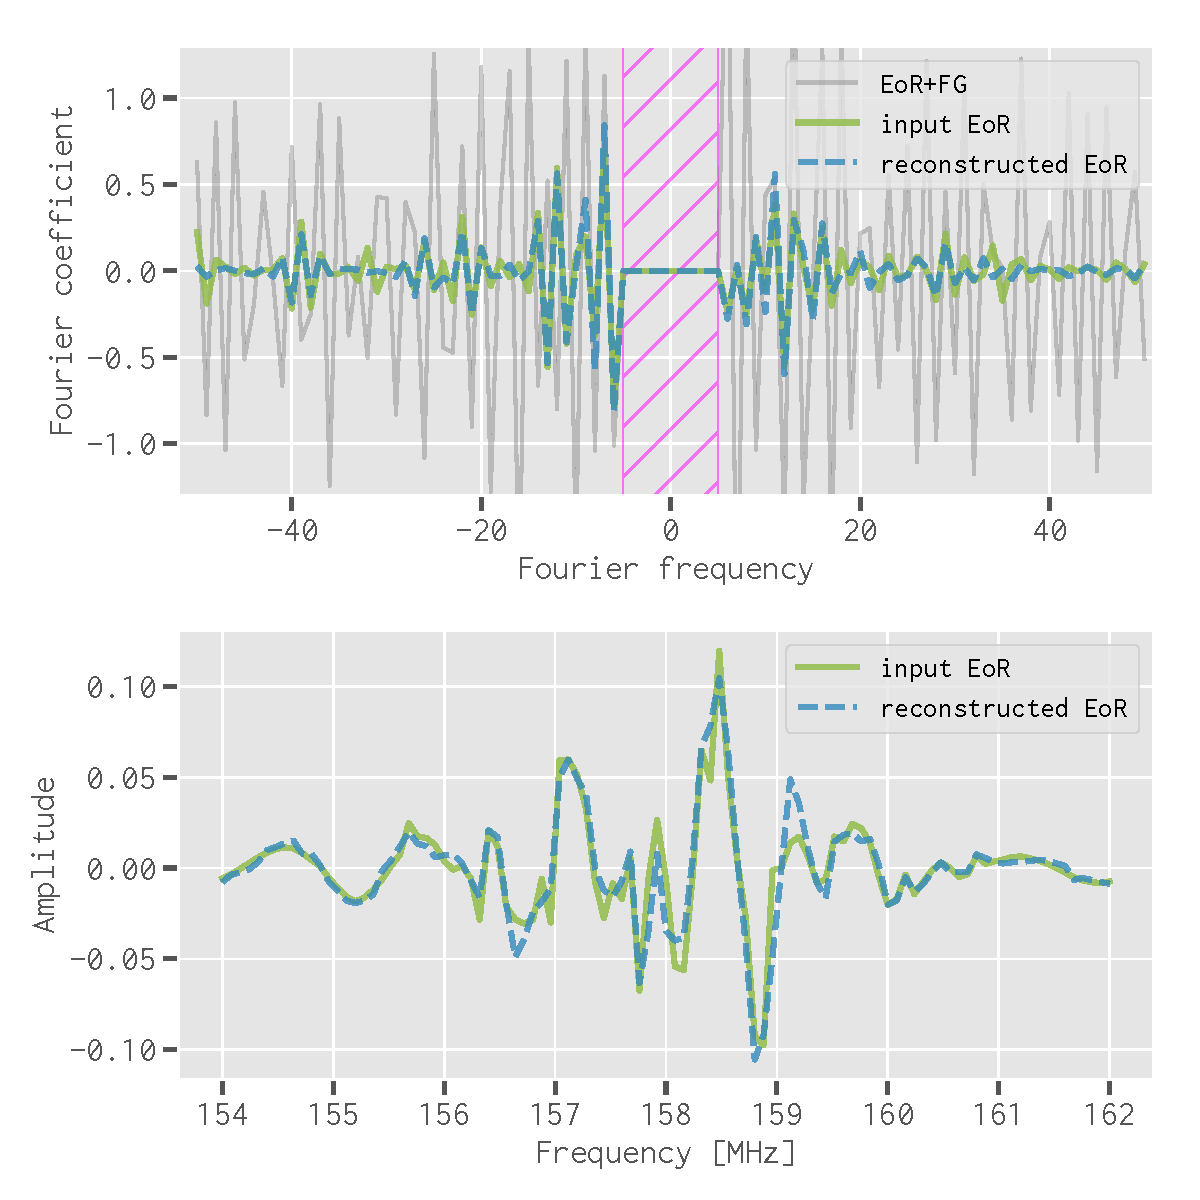
\includegraphics[height=0.8\textheight]{cdae-eor-pix}
      \end{figure}
  \end{itemize}
\end{frame}

\begin{frame}
  \vspace{1ex}
  \begin{itemize}
    \item 重建图像的空间结构与强度分布与输入几乎完全相同 \\
      {\small(小尺度波纹结构源自预处理时去除了低频 Fourier 系数)}
      \begin{figure}
        \centering
        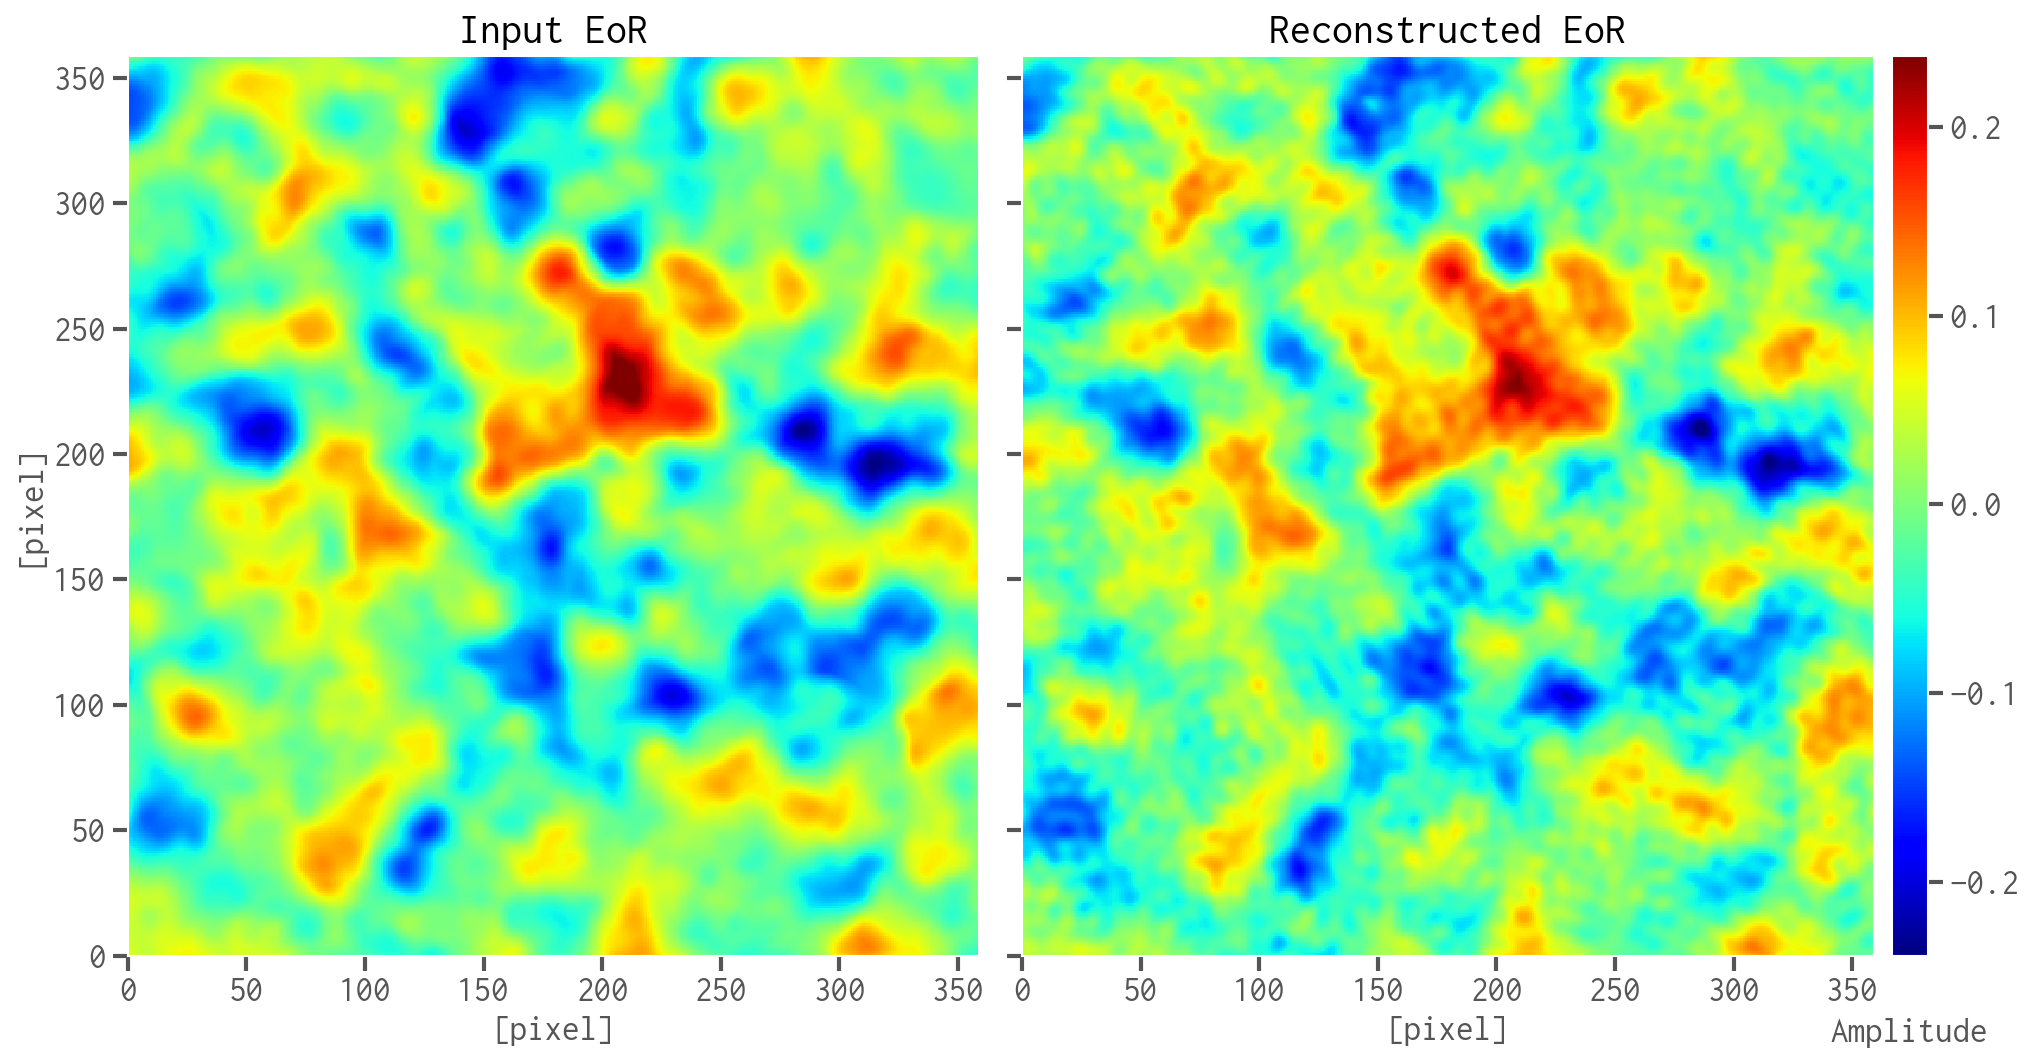
\includegraphics[height=0.44\textheight]{cdae-eor-img-comp}
      \end{figure}
    \item CDAE 很好地恢复了 EoR 信号在各尺度的功率:
      \begin{figure}
        \centering
        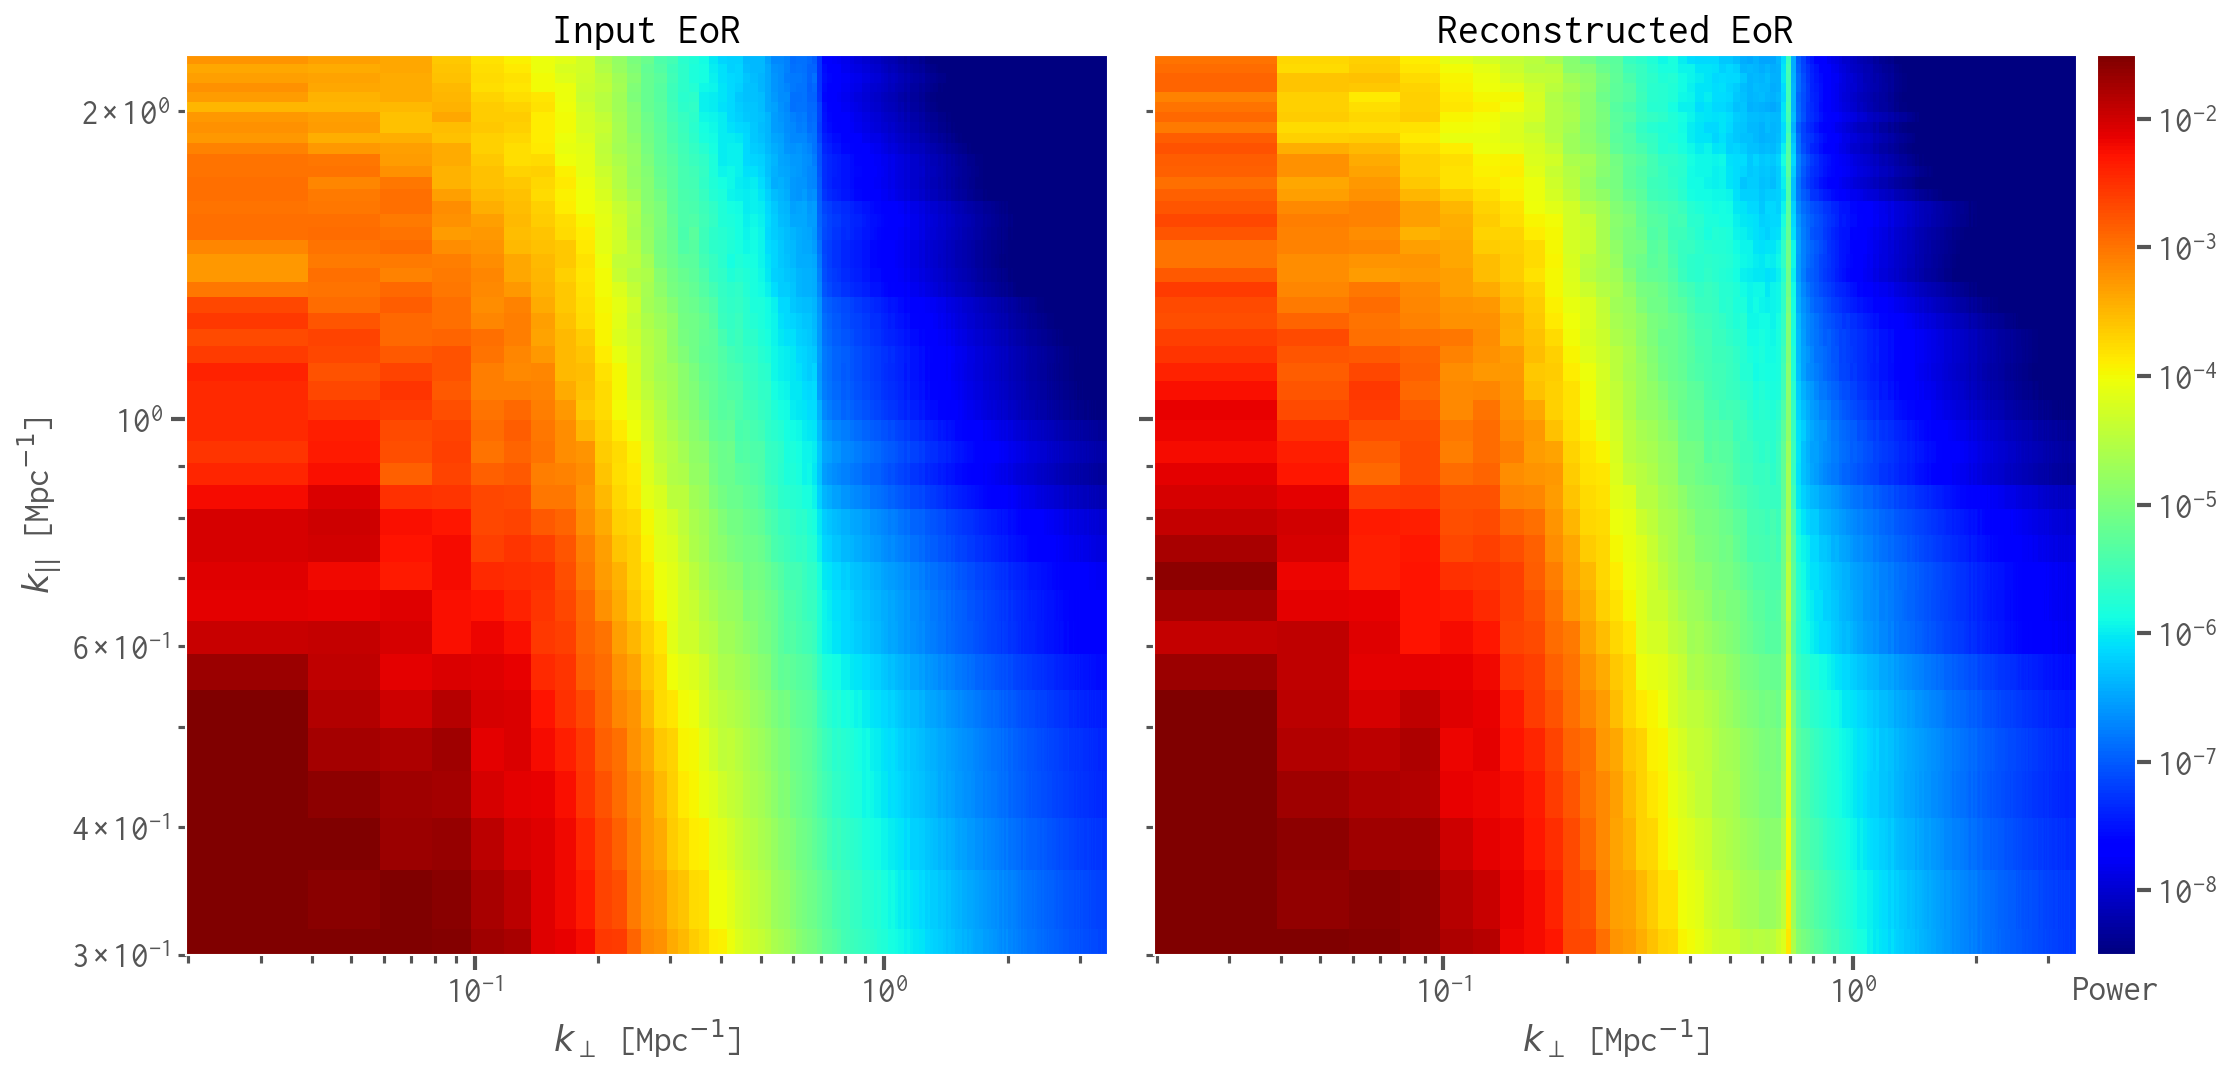
\includegraphics[height=0.44\textheight]{cdae-eor-ps-comp}
      \end{figure}
  \end{itemize}
\end{frame}

%............
\begin{frame}[subsec]
  \frametitle{与传统前景扣除方法的对比}
  \begin{table}
    \centering
    \begin{tabular}{cc}
      \toprule
      方法 & 分离效果 ($\bar{\xi}$) \\
      \midrule
      CDAE & \num{0.929 +- 0.045} \\
      \midrule
      多项式拟合法 & \num{0.296 +- 0.121} \\
      连续小波变换法 & \num{0.198 +- 0.160} \\
      \bottomrule
    \end{tabular}
  \end{table}
\end{frame}


%=====================================================================
\section{总结}

\begin{frame}{总\cspace{}结}
  \begin{itemize}
    \item 改进了射电晕的低频射电天图的模拟,整合了 SKA1-Low 阵列的仪器效应,
      获得了更逼真的 EoR 前景模型
    \item 定量评估了射电晕辐射对 EoR 信号探测的影响,
      说明了射电晕是一个有待重视的较强前景干扰成分
    \item 基于深度学习设计了一个卷积去噪自编码器,
      准确地分离出 EoR 信号,效果显著优于传统方法
  \end{itemize}

  程序、文档和论文均已公开在
  \href{https://github.com/liweitianux/}{Github}:\\
  \href{https://github.com/liweitianux/fg21sim}{fg21sim},
  \href{https://github.com/liweitianux/cdae-eor}{cdae-eor},
  \href{https://github.com/liweitianux/atoolbox}{atoolbox},
  \href{https://github.com/liweitianux/paper-halo-eor}{paper-halo-eor},
  \href{https://github.com/liweitianux/paper-eor-detection}{paper-eor-detection},
  \href{https://github.com/liweitianux/phd-thesis}{phd-thesis}
\end{frame}

\begin{frame}{已发表论文}
  \small
  \begin{itemize}
    \item
      \textsc{\alert{Li, Weitian}; Xu, Haiguang; Ma, Zhixian; Hu, Dan;
      Zhu, Zhenghao; Shan, Chenxi; Wang, Jingying; Gu, Junhua;
      Zheng, Dongchao; Lian, Xiaoli; Zheng, Qian; Wang, Yu;
      Zhu, Jie; Wu, Xiang-Ping}.
      \enquote{\it Contribution of Radio Halos to the Foreground for
        SKA EoR Experiments,}
      \href{http://adsabs.harvard.edu/abs/2019ApJ...879..104L}{%
        2019, ApJ, 879, 104}
    \item
      \textsc{\alert{Li, Weitian}; Xu, Haiguang; Ma, Zhixian; Zhu, Ruimin;
      Hu, Dan; Zhu, Zhenghao; Gu, Junhua; Shan, Chenxi; Zhu, Jie;
      Wu, Xiang-Ping}.
      \enquote{\it Separating the EoR Signal with a Convolutional Denoising
        Autoencoder: A Deep-learning-based Method,}
      \href{http://adsabs.harvard.edu/abs/2019MNRAS.485.2628L}{%
        2019, MNRAS, 485, 2628}
    \item
      合作论文 12 篇
  \end{itemize}
\end{frame}

\begin{frame}[standout]
  \huge 请各位老师批评指正,谢谢!
\end{frame}


%=====================================================================
\appendix

\begin{frame}[standout]
  Backup slides
\end{frame}

%---------------------------------------------------------------------
\subsection{射电天文学}

%............
\begin{frame}[subsec]
  \frametitle{射电天文学}
  \alert{射电天文学}:
  在射电波段对天体和宇宙开展研究的天文学分支.
  \alert{射电窗口}的频率范围 $\sim$ \SI{10}{\MHz} -- \SI{1000}{\GHz}.

  \begin{figure}
    \centering\footnotesize
    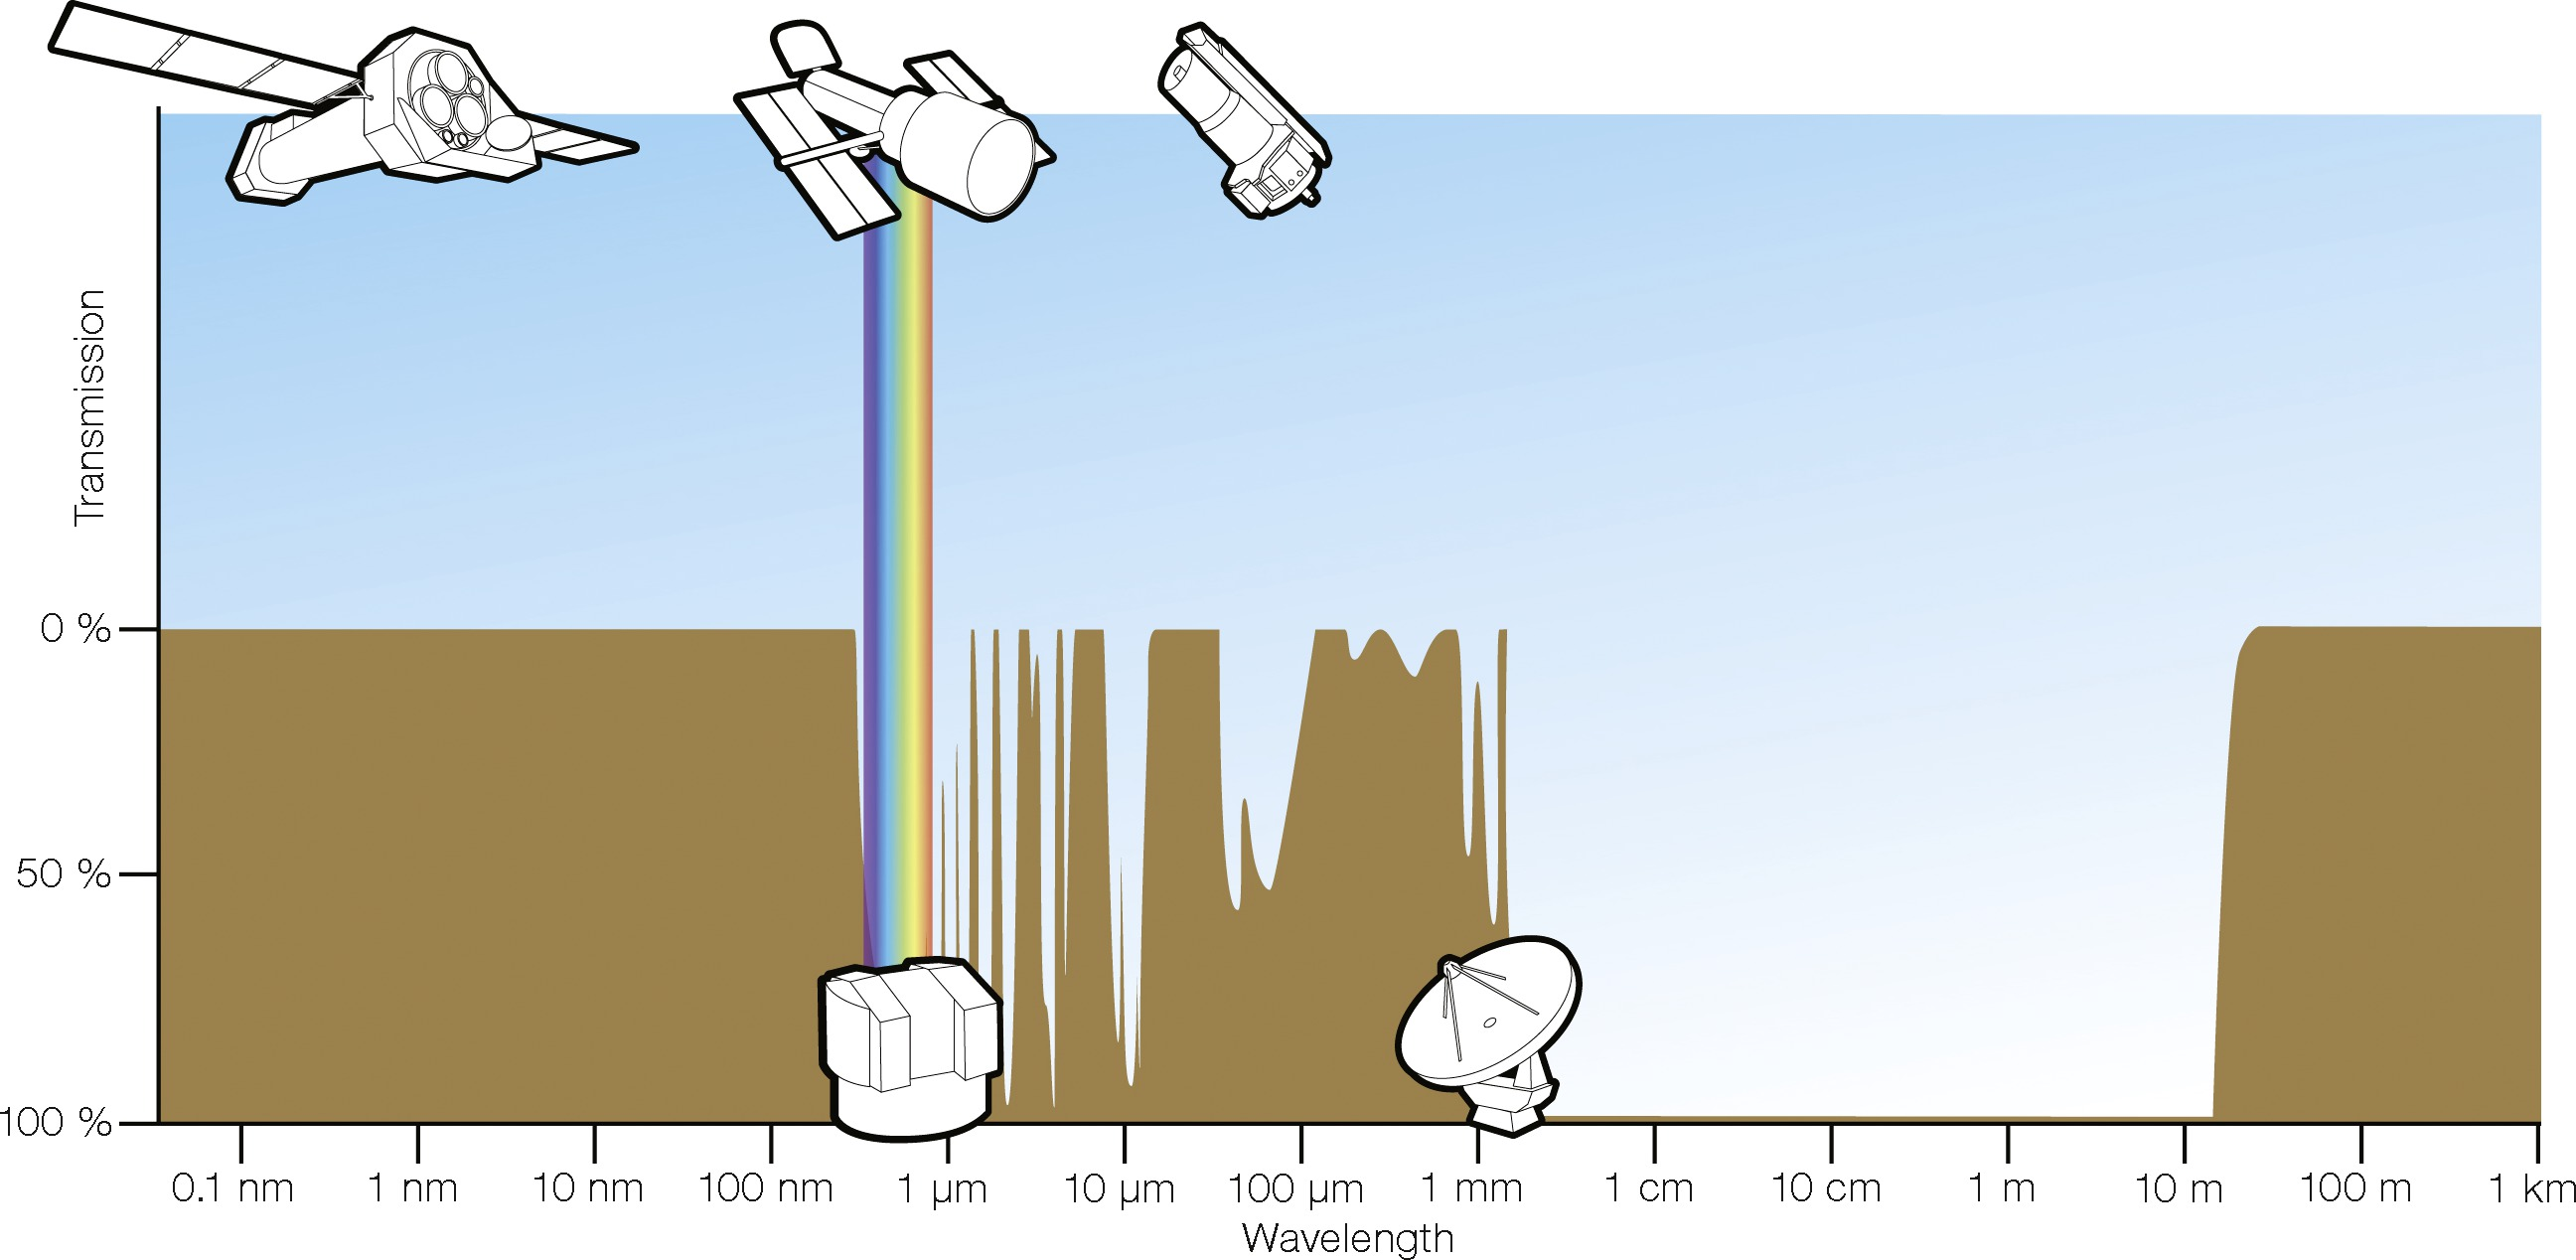
\includegraphics[width=\textwidth]{atmospheric-em-transmittance}
    大气层的电磁辐射透射率
  \end{figure}

  \vspace*{0.5em}
  \blfootnote{图片来源: \cite{condon2016}}
\end{frame}

%---------------------------------------------------------------------
\subsection{基本概念}

%............
\begin{frame}[subsec]
  \frametitle{比强度和流量密度}
  \begin{columns}[onlytextwidth]
    \column{0.6\textwidth}
      \begin{alertblock}{比强度 (specific intensity)}
        \smallskip
        单位频率间隔内、沿着辐射传播方向上单位立体角穿过垂直于传播方向的单位面积
        的辐射功率,即:
        \begin{equation}
          I_{\nu} \equiv
            \frac{\D{P_{\nu}}}{(\cos\theta\,\D{\sigma})
              \,\D{\nu} \,\D{\Omega}} .
        \end{equation}
      \end{alertblock}

      \begin{alertblock}{流量密度 (flux density)}
        \smallskip
        \begin{equation}
          S_{\nu} \equiv
            \int_{\R{source}} I_{\nu}(\theta,\phi) \cos\theta \,\D{\Omega} ,
        \end{equation}
        单位为 \si{\jansky},
        $\SI{1}{\jansky} = \SI{e-26}{\watt\per\square\meter\per\hertz}$.
      \end{alertblock}

    \column{0.35\textwidth}
      \begin{figure}
        \centering
        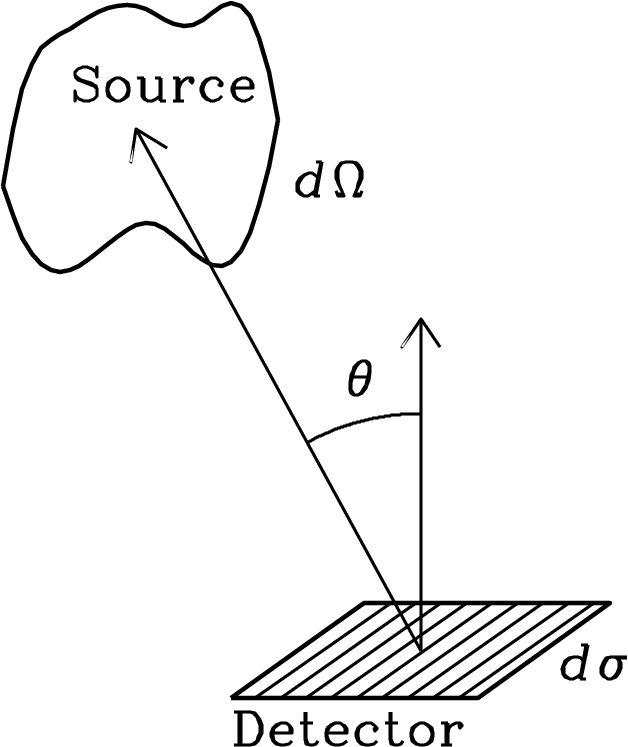
\includegraphics[width=\columnwidth]{specific-intensity}
      \end{figure}
  \end{columns}

  \blfootnote{图片来源: \cite{condon2016}}
\end{frame}

%............
\begin{frame}[subsec]
  \frametitle{黑体辐射和亮温度}
  \begin{itemize}
    \item \alert{黑体辐射}的频谱 $B_{\nu}(\nu, T)$ 只取决于其温度 $T$,
      由 \alert{Planck 定律}给出:
      \begin{equation}
        B_{\nu}(\nu, T) =
          \frac{2 h_p \nu^3}{c^2} \left[ \exp\left(
            \frac{h_p \nu}{k_B T} \right) - 1 \right]^{-1} .
      \end{equation}
    \item 在射电波段有 $h_p \nu \ll k_B T$,于是有 \alert{Rayleigh--Jeans 近似}:
      \begin{equation}
        B_{\nu}(\nu, T) \approx \frac{2 \nu^2 k_B T}{c^2} .
      \end{equation}
      黑体的亮度 $B_{\nu}$ 与其温度 $T$ 严格成正比.
    \item 一个辐射源的亮度 $I_{\nu}$ 可以很方便与使用\alert{亮温度}来描述:
      \begin{equation}
        T_b(\nu) \equiv \frac{I_{\nu} c^2}{2 k_B \nu^2} .
      \end{equation}
  \end{itemize}
\end{frame}

%............
\begin{frame}[subsec]
  \frametitle{辐射转移方程和光深}
  \begin{itemize}
    \item 辐射在介质中传播时会经历吸收和发射,由\alert{辐射转移方程}描述:
      \begin{equation}
        \diff{I_{\nu}}{s} = -\kappa I_{\nu} + j_{\nu} ,
      \end{equation}
      其中 $\kappa$ 为吸收系数, $j_{\nu}$ 为发射系数.
    \item \alert{光深}:
      \begin{equation}
        \tau \equiv
          - \int_{s_{\R{out}}}^{s_{\R{in}}} \kappa(s') \,\D{s'} .
      \end{equation}
      当 $\tau \ll 1$ 时,称介质是\emph{光学薄}的;
      当 $\tau \gg 1$ 时,则称介质是\emph{光学厚}的.
  \end{itemize}
\end{frame}

%---------------------------------------------------------------------
\subsection{干涉测量原理}

%............
\begin{frame}[subsec]
  \frametitle{干涉测量的基本原理}
  \begin{columns}[onlytextwidth]
    \column{0.38\textwidth}
    二元单色干涉仪观测一个点源,相关器的输出响应为:
    \begin{align}
      R & = \langle V_1(t) V_2(t) \rangle \\
        & = \frac{1}{2} V^2 \cos (\omega \tau_g) ,
    \end{align}
    $\tau_g = \B{b} \cdot \hat{\B{s}}$ 为几何延迟,\\
    $\B{b}$ 为基线矢量,\\
    $\hat{\B{s}}$ 为辐射源的方向.

    \column{0.55\textwidth}
    \begin{figure}
      \centering
      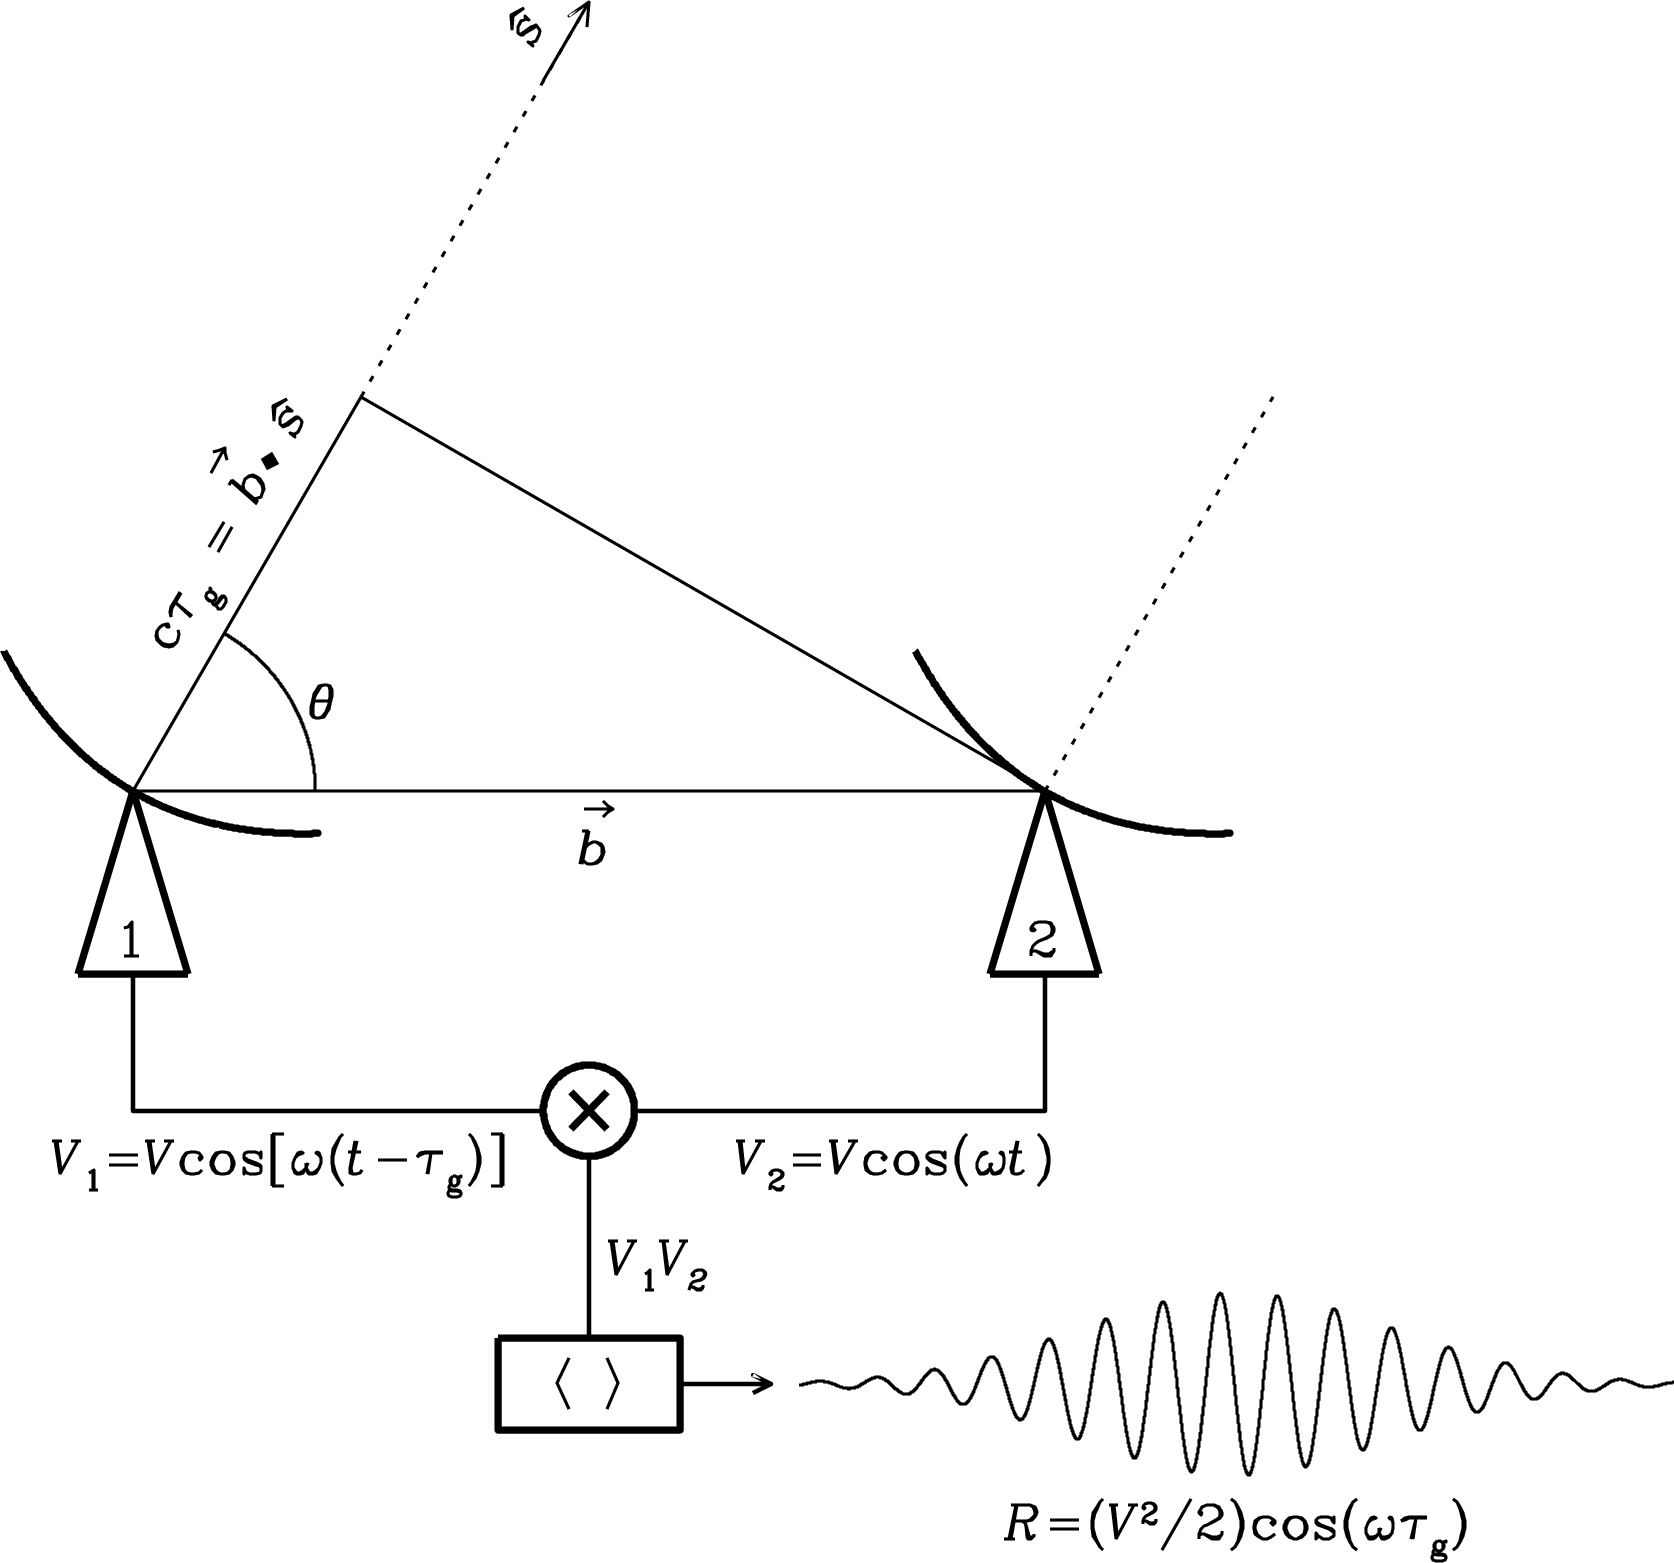
\includegraphics[width=\columnwidth]{interferometer}
    \end{figure}
  \end{columns}

  \blfootnote{图片来源: \cite{condon2016}}
\end{frame}

%............
\begin{frame}
  \begin{itemize}
    \item 一个展源 $I_{\nu}(\hat{\B{s}})$ 可当作一系列独立的点源处理,
      于是干涉仪响应为:
      \begin{equation}
        R_c = \int I_{\nu}(\hat{\B{s}})
          \cos (2\Cpi\, \B{b} \cdot \hat{\B{s}} / \lambda) \,\D{\Omega} .
      \end{equation}
    \item 上述 \enquote{cosine} 相关器只能测量 $I_{\nu}(\hat{\B{s}})$ 的偶成分.
    \item 为测量 $I_{\nu}(\hat{\B{s}})$ 的奇成分,
      还需要一个 \enquote{sine} 相关器,
      可通过对其中一个天线的输出增加 $\Cpi/2$ 的相位延迟来实现,于是:
      \begin{equation}
        R_s = \int I_{\nu}(\hat{\B{s}})
          \sin (2\Cpi\, \B{b} \cdot \hat{\B{s}} / \lambda) \,\D{\Omega} .
      \end{equation}
    \item \alert{复可见度 (complex visibility)} 定义为:
      \begin{equation}
        \mathcal{V}
          \equiv R_c - \Ci R_s
          = \int I_{\nu}(\hat{\B{s}})
            \exp (- 2\Cpi\Ci\, \B{b} \cdot \hat{\B{s}} / \lambda)
            \,\D{\Omega} .
      \end{equation}
  \end{itemize}
\end{frame}

%............
\begin{frame}[subsec]
  \frametitle{干涉成像坐标系统}
  \begin{columns}[onlytextwidth]
    \column{0.55\textwidth}
    \begin{itemize}
      \item $w$ 轴指向参考方向,通常为目标的中心; \\
        $u$ 轴向东; \\
        $v$ 轴向北.
      \item 基线矢量: $\B{b} = (u,v,w) \,\lambda$.
      \item 方向矢量: $\hat{\B{s}} = \left( l, m, \sqrt{1-l^2-m^2} \right)$,
        其中 $l, m$ 分别为 $\hat{\B{s}}$ 对 $u, v$ 轴的投影长度.
    \end{itemize}

    \column{0.4\textwidth}
    \begin{figure}
      \centering
      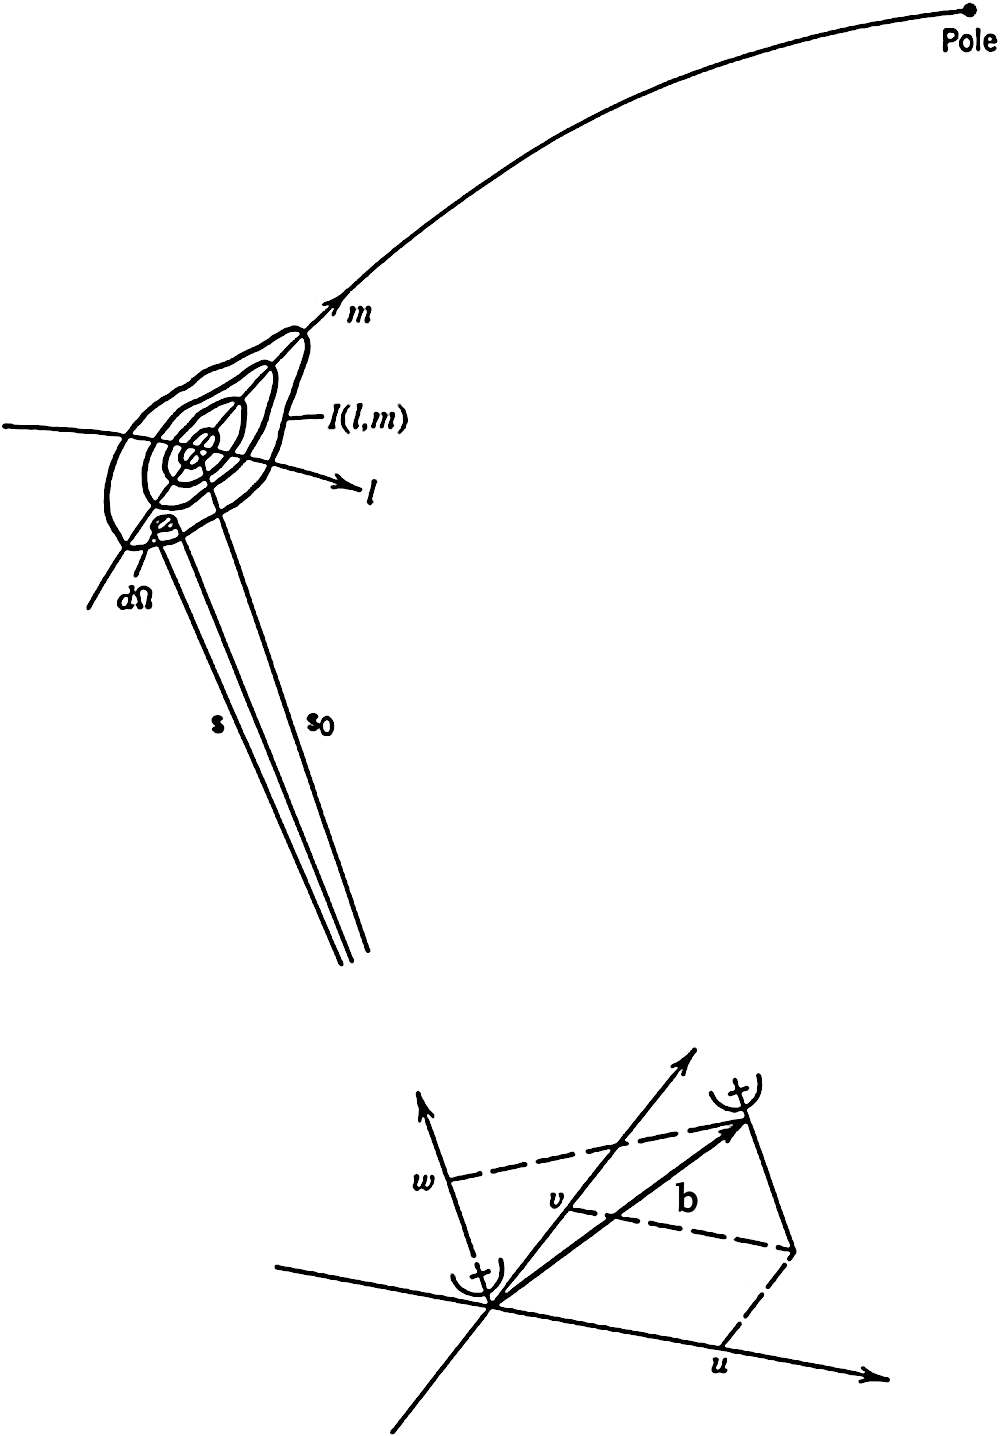
\includegraphics[width=\columnwidth]{interferometer-coordsys}
    \end{figure}
  \end{columns}

  \blfootnote{图片来源: \cite{thompson2017}}
\end{frame}

%............
\begin{frame}[subsec]
  \frametitle{干涉成像原理}
  \vspace{-1ex}
  \begin{equation}
    \mathcal{V}(u,v,w)
      = \!\iint \!\frac{I_{\nu}(l,m)}{\sqrt{1-l^2-m^2}}
      \exp \!\left[ -2\Cpi\Ci \!\left( ul+vm+w\sqrt{1-l^2-m^2} \right) \right]
      \D{l}\,\D{m}
  \end{equation}

  \begin{itemize}
    \item 注意,上式\alert{不是}二维 Fourier 变换.
    \item 在以下两种常见的特殊情况下:
      \begin{itemize}
        \item 所有基线矢量共面,即有 $w = 0$;
        \item 小视场成像,即满足 $\big| \Cpi w(l^2+m^2) \big| \ll 1$.
      \end{itemize}
      上式可近似成二维 Fourier 变换:
      \begin{equation}
        \mathcal{V}(u,v)
          = \iint \frac{I_{\nu}(l,m)}{\sqrt{1-l^2-m^2}}
            \exp [-2\Cpi\Ci\, (ul+vm)] \,\D{l}\,\D{m},
      \end{equation}
    \item 通过逆变换,可得目标的亮度分布 $I_{\nu}(l,m)$:
      \begin{equation}
        \frac{I_{\nu}(l,m)}{\sqrt{1-l^2-m^2}}
          = \iint \mathcal{V}(u,v)
            \exp [2\Cpi\Ci\, (ul+vm)] \,\D{l}\,\D{m}.
      \end{equation}
  \end{itemize}
\end{frame}

%............
\begin{frame}[subsec]
  \frametitle{$uv$ 覆盖和脏图}
  \begin{itemize}
    \item 基线 $\B{b} = (u,v,w) \,\lambda$ 每个时刻测量一对可见度数据: \\
      $\mathcal{V}(u,v)$ 和 $\mathcal{V}(-u,-v)$.
    \item \alert{$uv$ 覆盖}指 $uv$ 平面内被测量到的范围,
      由\alert{采样函数} $S(u,v)$ 描述.
    \item 对测量的可见度数据进行逆 Fourier 变换,
      仅能得到目标的\alert{脏图 (dirty map)}:
      \begin{equation}
        \frac{I_{\nu}^D(l,m)}{\sqrt{1-l^2-m^2}}
          = \iint \mathcal{V}(u,v) S(u,v)
            \exp [2\Cpi\Ci\, (ul+vm)] \,\D{l}\,\D{m}.
      \end{equation}
    \item \alert{综合波束 (synthesized beam)}
      或\alert{点扩散函数 (point spread function; PSF)}
      是 $S(u,v)$ 的 Fourier 变换:
      \begin{equation}
        B(l,m) = \iint S(u,v) \exp [2\Cpi\Ci\, (ul+vm)] \,\D{l}\,\D{m}.
      \end{equation}
  \end{itemize}
\end{frame}

%............
\begin{frame}[subsec]
  \frametitle{成像过程的变换关系}
  \vspace{-1ex}
  \begin{equation}
    I_{\nu}^D(l,m) = I_{\nu}(l,m) * B(l,m)
  \end{equation}
  \begin{center}
    \footnotesize\noindent
    真实天图 \hspace{4em} 综合波束 \hspace{4.5em} 脏图 \\
    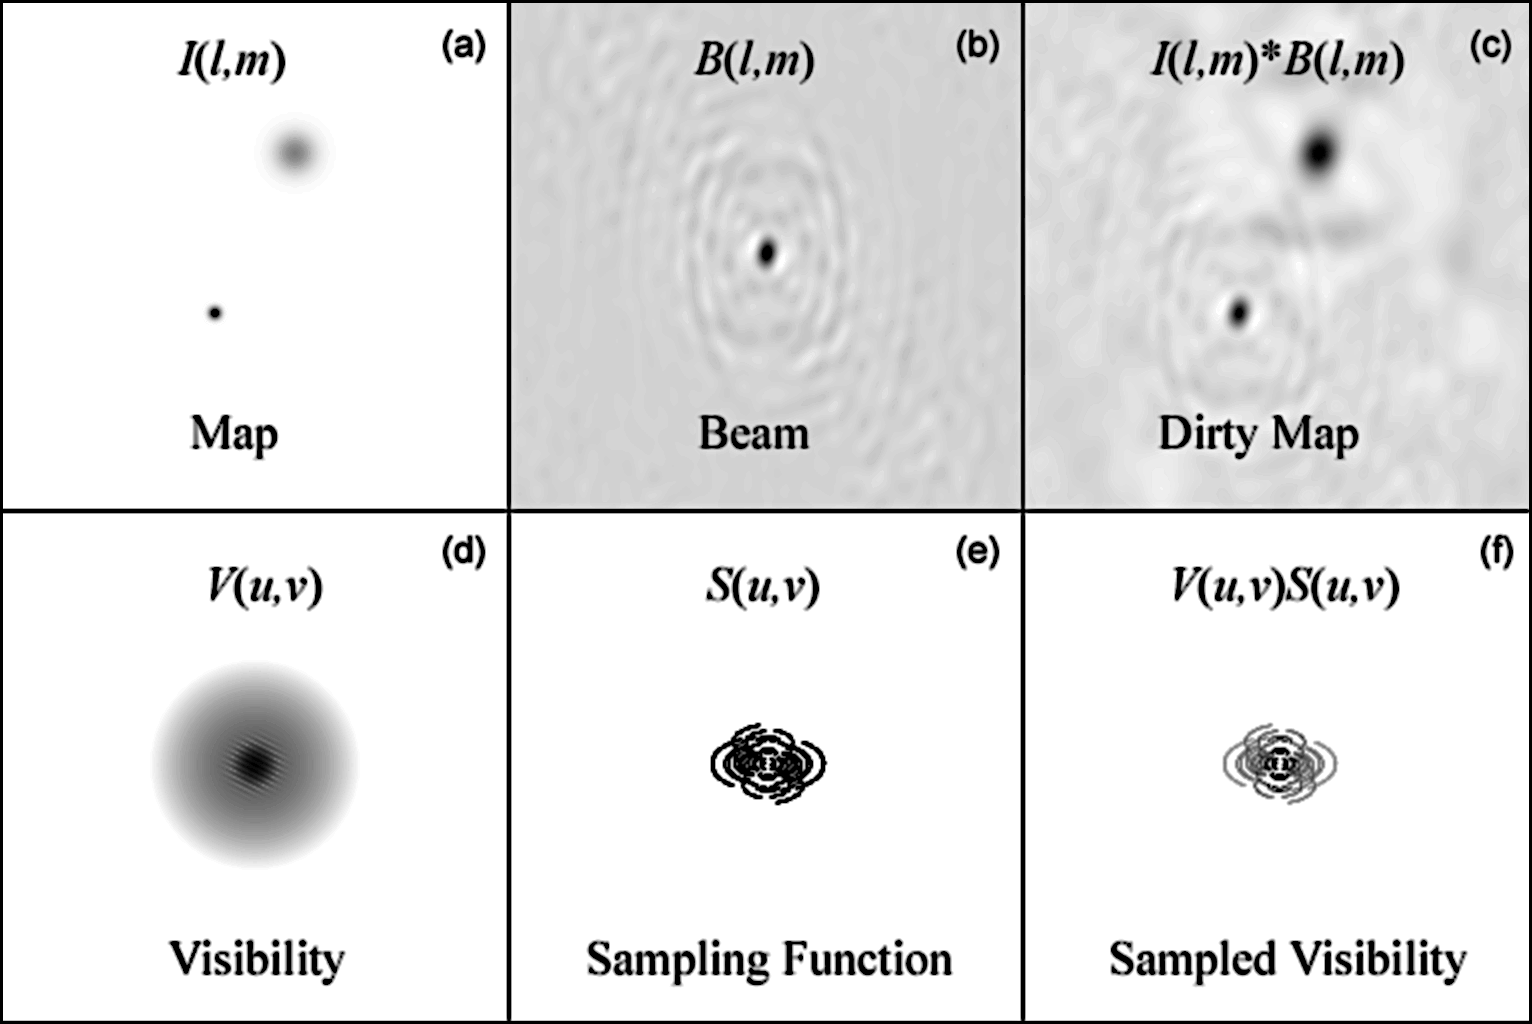
\includegraphics[width=0.75\textwidth]{imaging-relations} \\
    真实的可见度 \hspace{2.5em} 采样函数 \hspace{3em} 测量的可见度
  \end{center}

  \vspace*{1em}
  \blfootnote{图片来源: Dale E. Gary, Radio Astronomy}
\end{frame}

%---------------------------------------------------------------------
\subsection{EoR 信号原理}

%............
\begin{frame}[subsec]
  \frametitle{中性氢 21\,cm 谱线}
  \begin{columns}[t,onlytextwidth]
    \column{0.55\textwidth}
    \begin{itemize}
      \item 质子和电子均有 1/2 自旋
      \item 两个自旋的相互作用使氢原子的基态发生\alert{超精细分裂}
      \item 当电子的自旋发生翻转时,会产生/吸收频率约为 \SI{1420}{\MHz} 的光子,
        波长约为 21\,cm,因此称为 \alert{21\,cm 谱线}
    \end{itemize}

    \column{0.45\textwidth}
    \begin{figure}
      \centering
      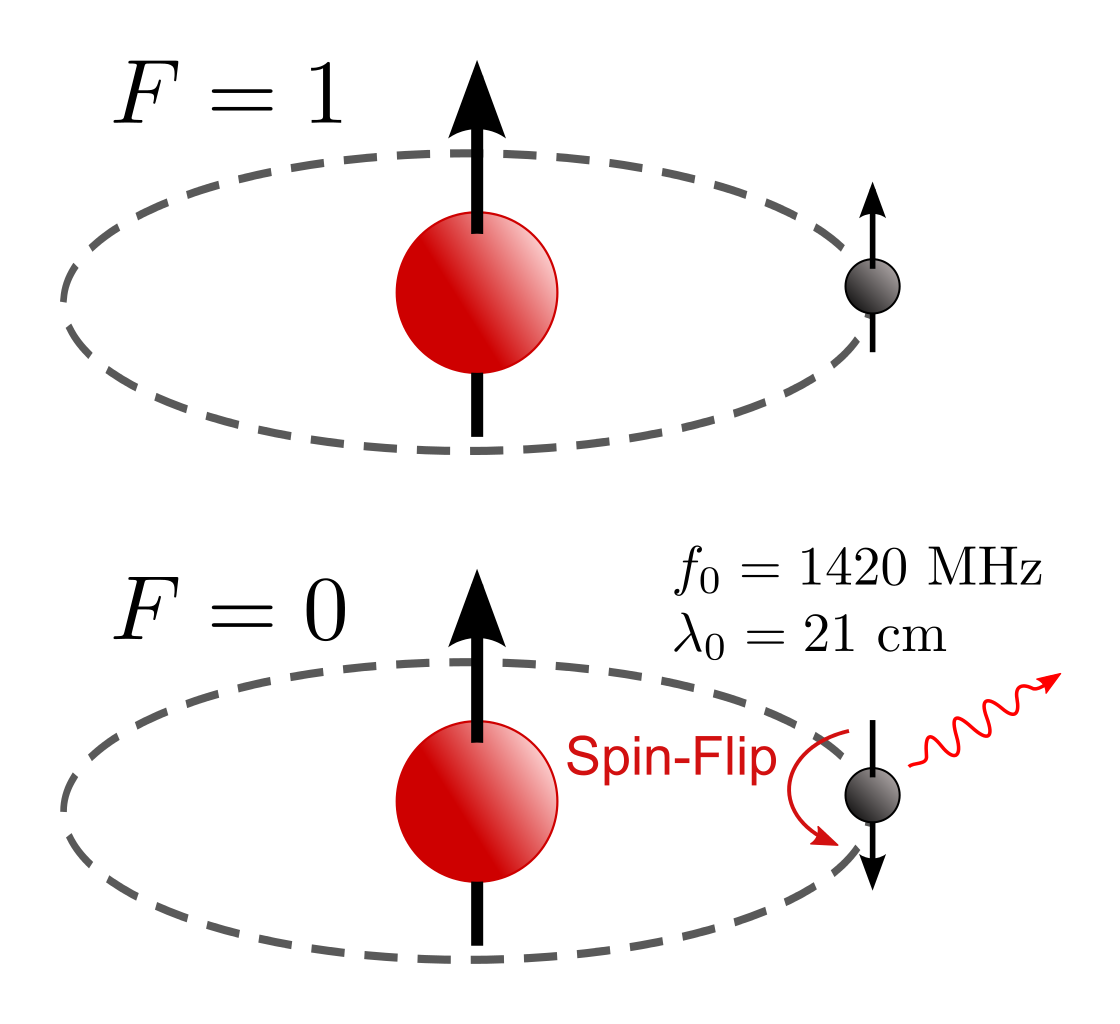
\includegraphics[width=\columnwidth]{hydrogen-spinflip}
    \end{figure}
  \end{columns}

  \blfootnote{图片来源: Tiltec, Wikipedia}
\end{frame}

%............
\begin{frame}{EoR 信号的亮温度}
  \begin{figure}
    \centering
    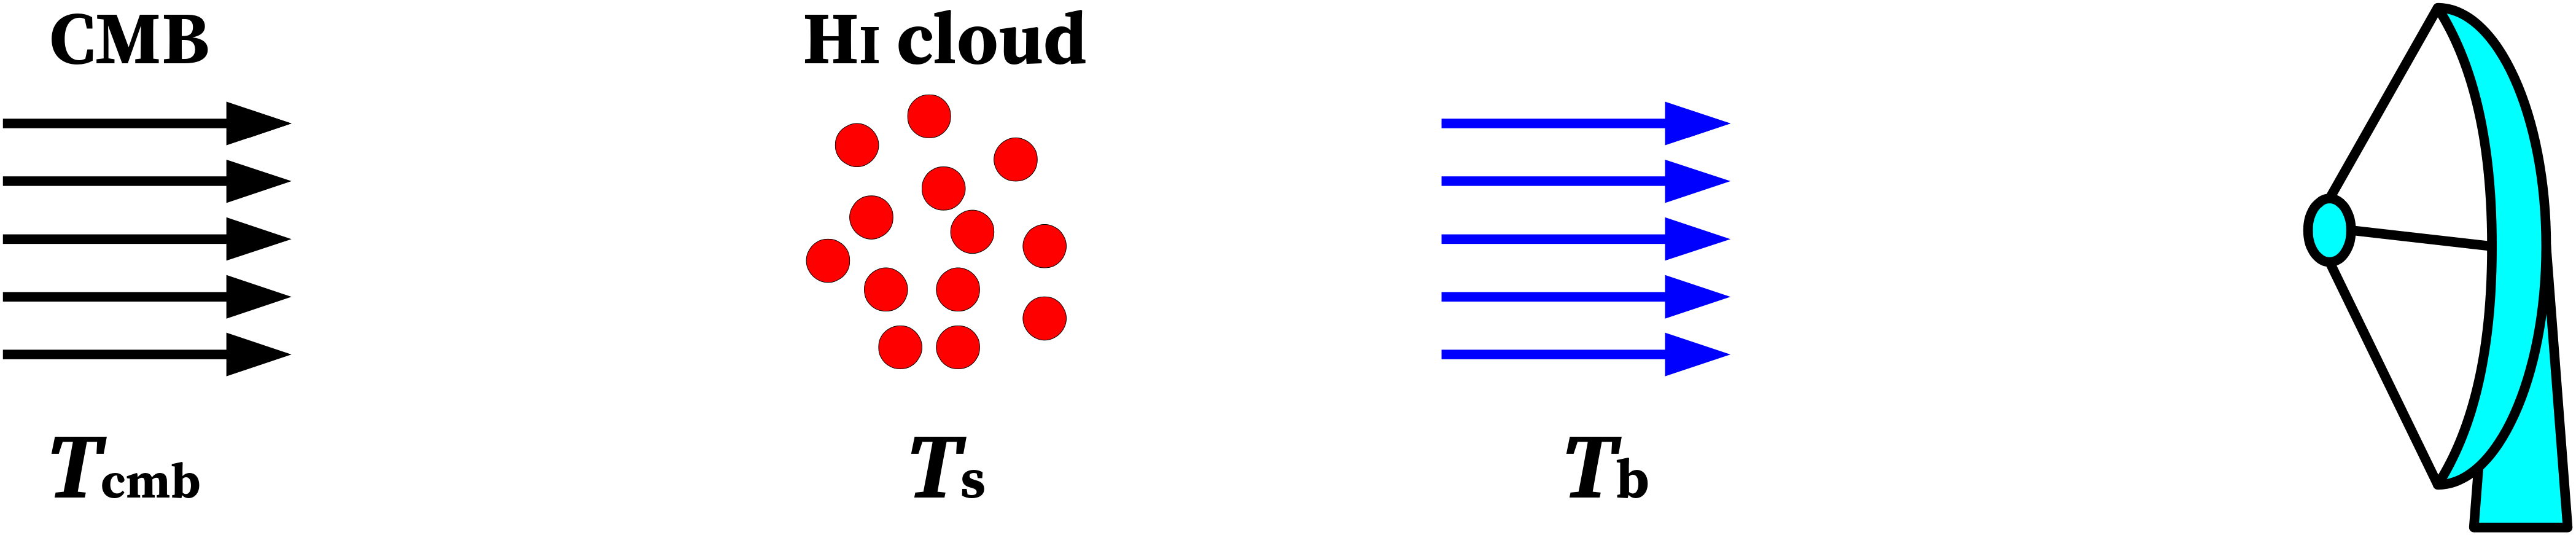
\includegraphics[width=\textwidth]{21cm-radiative-transfer}
  \end{figure}

  待探测的 \alert{EoR 信号}为中性氢云的辐射相对于 CMB 辐射的\alert{差异}:
  \begin{equation}
    \delta T_b(\nu) \approx
      \frac{3 h_p c^3 A_{21}}{32\Cpi \nu_0^2 \,k_B}
      \frac{\chi_{\R{HI}} n_{\R{HI}}}{
        (1+z)^2 (\partial v_{\parallel} / \partial r_{\parallel})}
      \left[ 1 - \frac{T_{\R{cmb}}(z)}{T_s} \right] ,
  \end{equation}
  其中 $A_{21}$ 为自发发射系数,
  $\chi_{\R{HI}}$ 为氢原子的中性比例, \\
  $n_{\R{HI}}$ 为数密度,$v$ 为自行速度,$T_s$ 为自旋温度,\\
  $T_{\R{cmb}}$ 为 CMB 辐射亮温度

  \vspace*{2em}
  \blfootnote{图片来源: \cite{zaroubi2013}}
\end{frame}

%............
\begin{frame}[subsec]
  \frametitle{EoR 信号随红移的演化}
  \begin{equation}
    \delta T_b(\nu) \propto
      \chi_{\R{HI}} n_{\R{HI}}
      \left[ 1 - \frac{T_{\R{cmb}}(z)}{T_s} \right]
  \end{equation}

  \begin{figure}
    \centering
    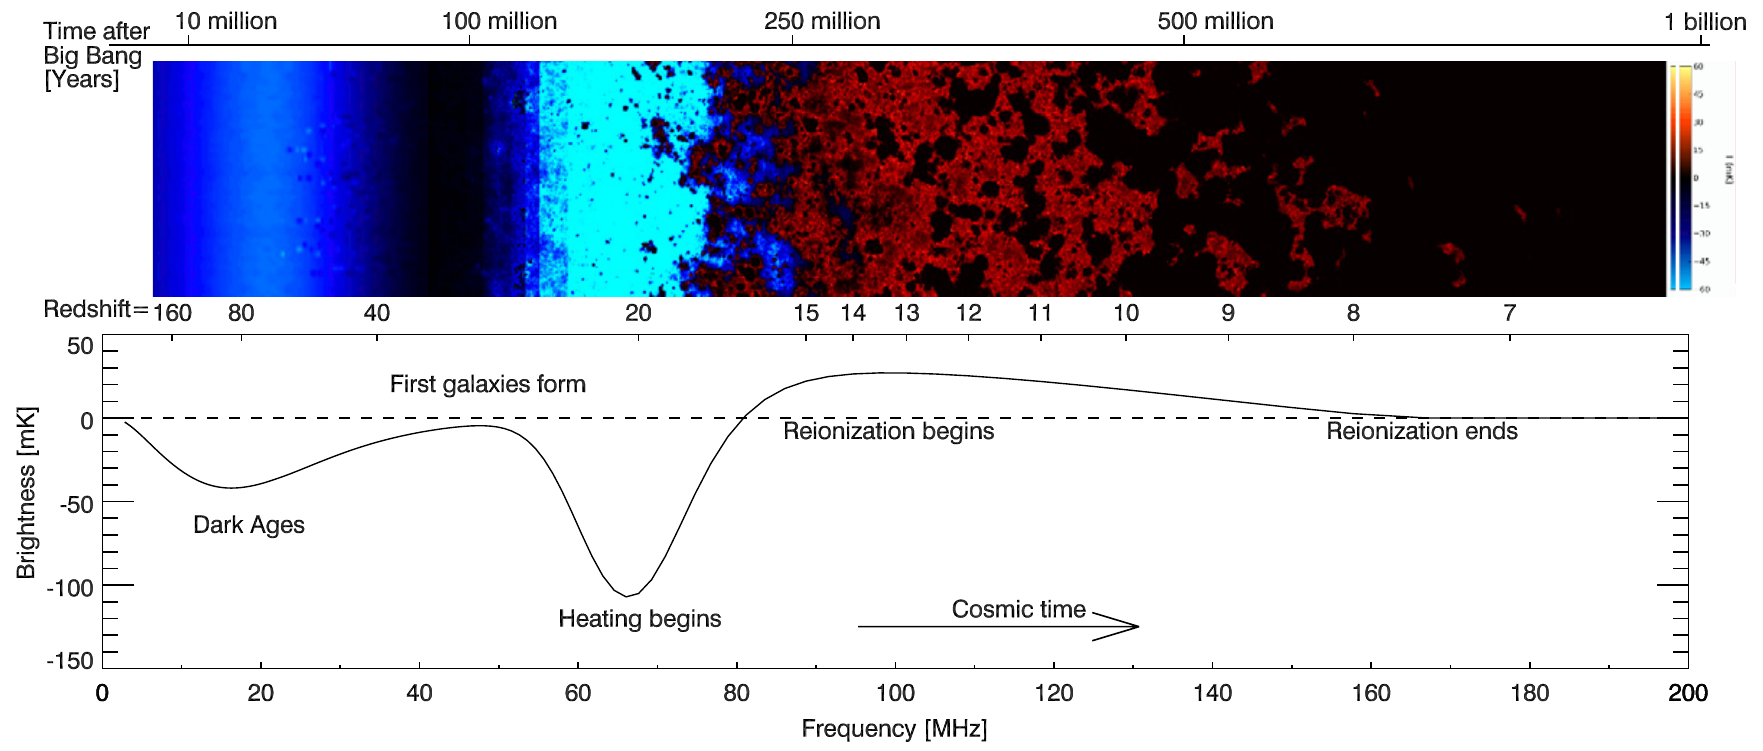
\includegraphics[width=\textwidth]{eor-signal-evolution}
  \end{figure}

  \blfootnote{图片来源: \cite{pritchard2012}}
\end{frame}

%---------------------------------------------------------------------
\subsection{模式混合}

%............
\begin{frame}[subsec]
  \frametitle{模式混合和前景楔形}
  \begin{itemize}
    \item \alert{色彩效应 (chromatic effect)}:
      一条基线的空间分辨率随频率的增大而提高,
      即所测量的波数正比于频率: $u = b/\lambda \propto \nu$
    \item 基线越长,色彩效应越显著
    \item 将 $k_{\perp}$ 模式里的功率\alert{混合}到 $k_{\parallel}$ 模式里,
      导致\alert{前景楔形}
  \end{itemize}

  \vspace{-1ex}
  \myfigure{%
    height=0.68\textheight,
    vertcap,
  }{chromatic-baselines}{%
    基线的色彩效应示意图
  }
\end{frame}

%---------------------------------------------------------------------
\subsection{射电晕建模}

%............
\begin{frame}[subsec]
  \frametitle{星系团的质量和红移分布}
  \begin{columns}[onlytextwidth]
    \column{0.49\textwidth}
    红移 $z$ 时每单位共动体积内质量范围 $[M,\, M+\D{M}]$ 的星系团数目:
    \begin{multline}
      n_{\R{cl}}(M,z) \,\D{M} =
        \sqrt{\frac{2}{\Cpi}} \frac{\langle \rho_0 \rangle}{M}
        \frac{\delta_c(z)}{\sigma^2(M)} \times \\
        \left| \diff{\sigma(M)}{M} \right|
        \exp\!\left[ -\frac{\delta_c^2(z)}{2\sigma^2(M)} \right]
        \,\D{M} ,
    \end{multline}
    $\langle \rho_0 \rangle$ 是当前的宇宙平均密度,
    $\delta_c(z)$ 是暗物质坍缩的临界密度,
    $\sigma(M)$ 是平均质量为 $M$ 的球形区域里的密度涨落值.

    \column{0.49\textwidth}
    \begin{figure}
      \centering
      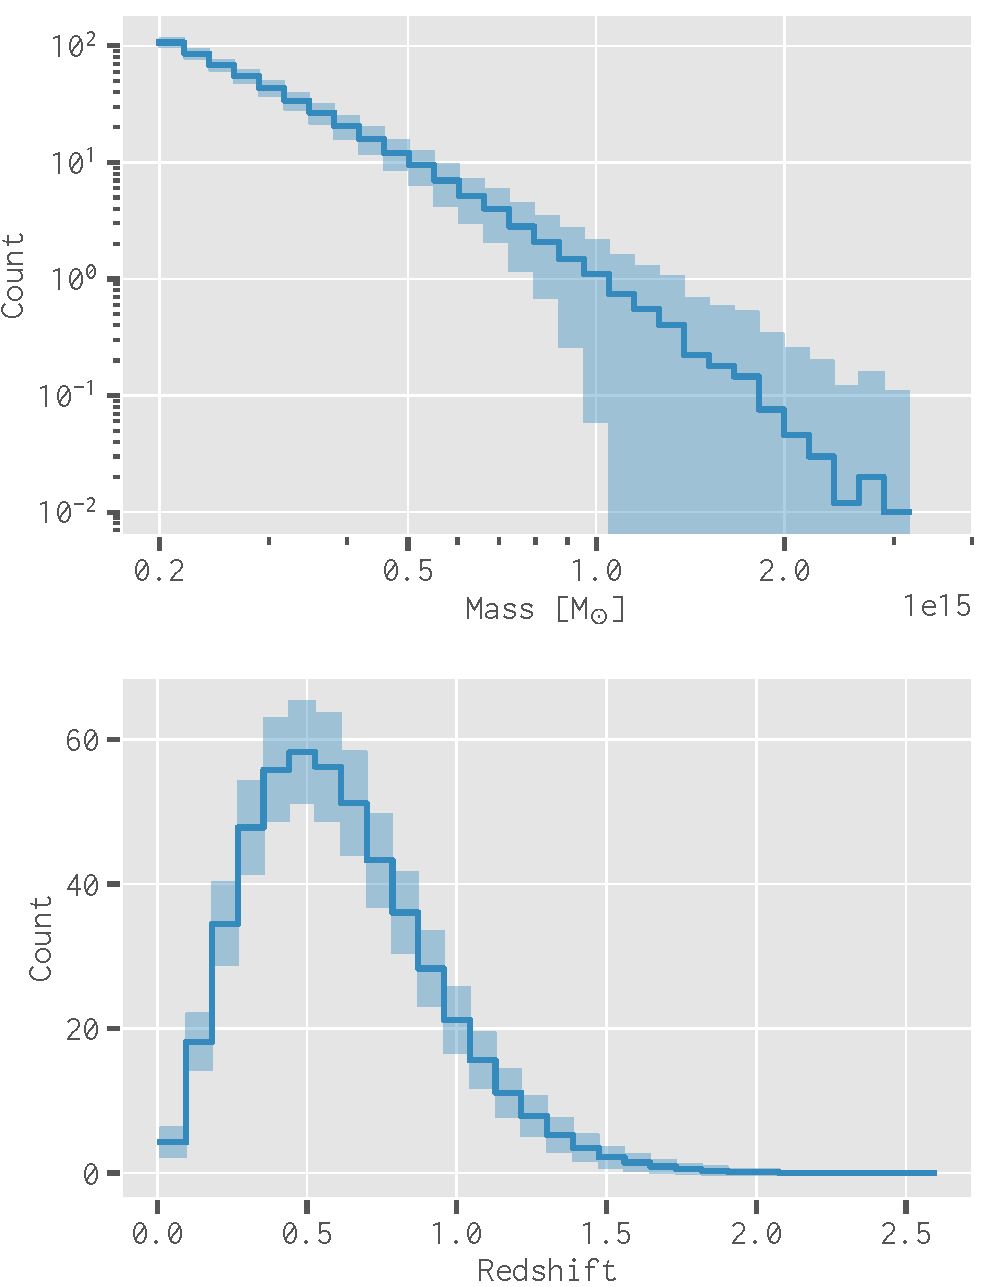
\includegraphics[width=\columnwidth]{mass-z-dist}
    \end{figure}
  \end{columns}
\end{frame}

%............
\begin{frame}[subsec]
  \frametitle{星系团并合历史的模拟}
  \begin{columns}[onlytextwidth]
    \column{0.49\textwidth}
    质量为 $M_2$ 的星系团在一个较早时刻 $t_1$ 具有一个质量范围为
    $[M_1,\, M_1+\D{M_1}]$ 的前身的条件概率为:
    \begin{multline}
      \R{Pr}(M_1, t_1 \,|\, M_2, t_2) \,\D{M_1} = \\
        \frac{1}{\sqrt{2\Cpi}} \frac{M_2}{M_1}
        \frac{\delta_{c1} - \delta_{c2}}{(\sigma_1^2 - \sigma_2^2)^{3/2}}
        \left| \diff{\sigma_1^2}{M_1} \right|
        \times \\
        \exp \!\left[ -\frac{(\delta_{c1} - \delta_{c2})^2}
        {2(\sigma_1^2 - \sigma_2^2)} \right] \,\D{M_1} .
    \end{multline}
    利用 Monte Carlo 模拟构建星系团\alert{并合树}.

    \column{0.49\textwidth}
    \begin{figure}
      \centering
      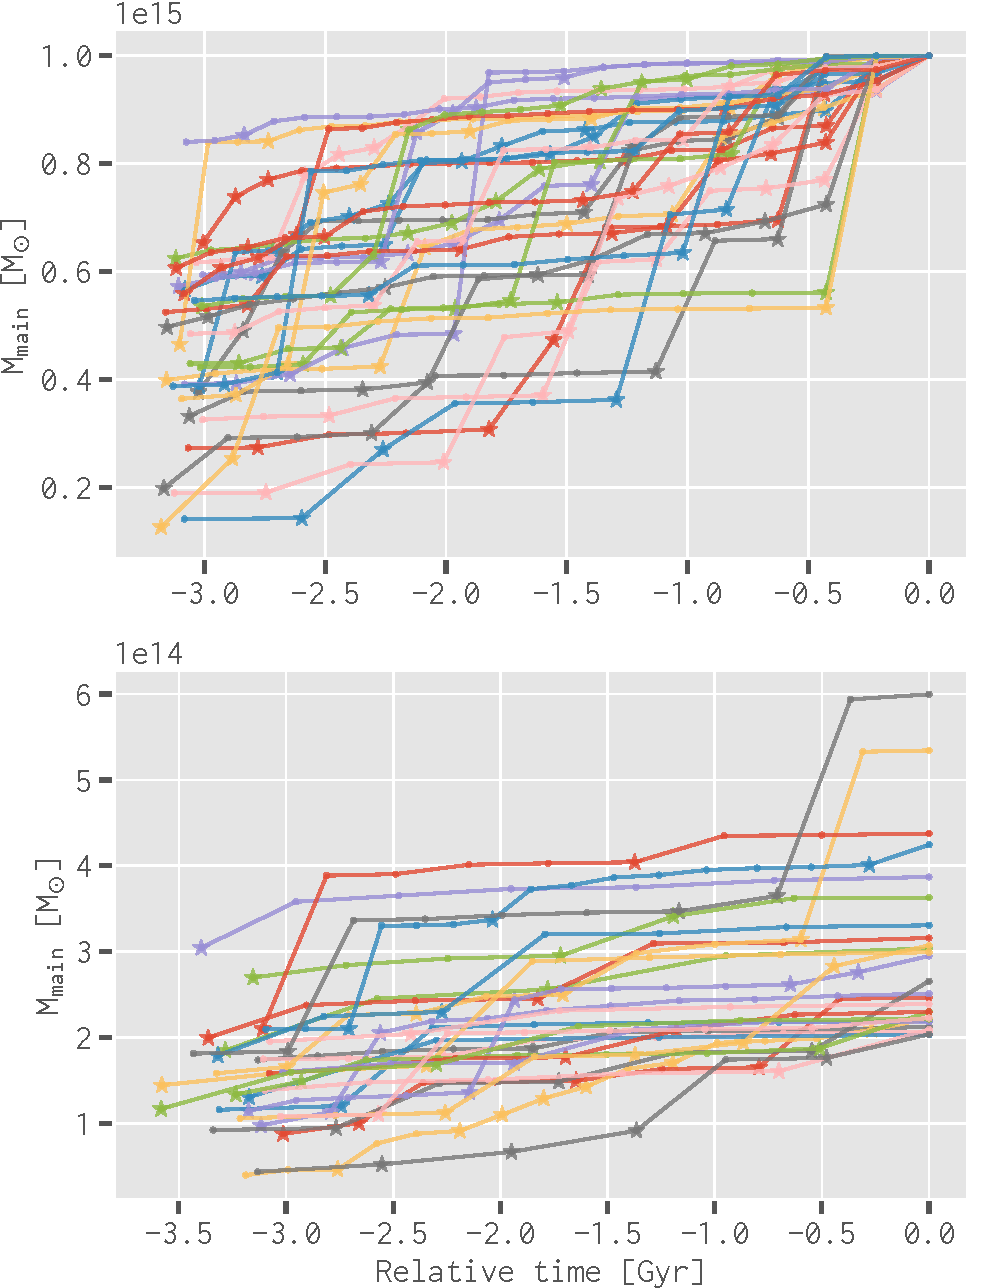
\includegraphics[width=\columnwidth]{merging-history}
    \end{figure}
  \end{columns}
\end{frame}

%............
\begin{frame}[subsec]
  \frametitle{高能电子的演化模型}
  在\alert{湍流再加速}和\alert{能量损失}的共同作用下,
  电子能谱 $n_e(\gamma, t)$ 随时间的演化由 \alert{FP 方程}描述:
  \begin{multline}
    \pdiff{n_e(\gamma, t)}{t} =
      \pdiff{}{\gamma} \left[ n_e(\gamma, t) \left(
        \left| \diff{\gamma}{t} \right| -
        \frac{2}{\gamma} D_{\gamma\gamma}(\gamma, t) \right) \right] + \\
      \pdiff{}{\gamma} \left[
      D_{\gamma\gamma} \pdiff{n_e(\gamma, t)}{\gamma} \right]
      + Q_e(\gamma, t) ,
  \end{multline}
  $D_{\gamma\gamma}$ 是描述湍流和电子相互作用的扩散系数,\\
  $|\R{d}\gamma / \R{d}t|$ 是能量损失速率,\\
  $Q_e$ 描述初级电子注入过程.
\end{frame}

%............
\begin{frame}[t]
  \begin{alertblock}{初级电子注入过程}
    \smallskip
    \begin{itemize}
      \item AGN 活动、恒星形成等过程持续地将初级电子注入 ICM
      \item 假定:
        \begin{itemize}
          \item 注入速率 $K_e$ 恒定
          \item 注入电子的能谱为幂律形式,谱指数为 $s$
          \item 注入电子的总能量密度与 ICM 热能密度 $\epsilon_{\R{th}}$
            之比为 $\eta_e$
        \end{itemize}
      \item 可得:
        \begin{align}
          Q_e(\gamma, t) & = K_e \gamma^{-s} , \\
          K_e & = \frac{(s-2) \eta_e \epsilon_{\R{th}}}{
            \epsilon_e \tau_{\R{cl}}} \gamma_{\R{min}}^{s-2} ,
        \end{align}
        其中 $\epsilon_e = m_e c^2$,
        $\tau_{\R{cl}}$ 为星系团年龄
    \end{itemize}
  \end{alertblock}
\end{frame}

%............
\begin{frame}[t]
  \begin{alertblock}{湍流再加速过程}
    \smallskip
    \begin{itemize}
      \item 湍流与 ICM 中的宇宙射线粒子发生作用而耗散能量,
        使初级电子获得能量而加速
      \item 该加速机制的扩散系数为:
        \begin{equation}
          D_{\gamma\gamma} =
            2 \gamma^2 \zeta k_L
            \frac{\langle (\delta v_t)^2 \rangle^2}{\chi_{\R{cr}} c_s^3} ,
        \end{equation}
        $\zeta$ 为 ICM 等离子体的不稳定性,\\
        $\chi_{\R{cr}}$ 为宇宙射线的能量密度与 ICM 热能密度之比,\\
        $k_L = 2\Cpi / r_{\R{turb}}$ 为湍流注入尺度,
        $c_s$ 为声速
      \item $\langle (\delta v_t)^2 \rangle$ 为湍流的速度弥散:
        \begin{equation}
          \langle (\delta v_t)^2 \rangle =
            \langle (\delta v_0)^2 \rangle +
            \frac{2 \eta_t E_m}{M_{\R{turb}}} ,
        \end{equation}
        $\eta_t$ 为并合注入湍流的能量比例
    \end{itemize}
  \end{alertblock}
\end{frame}

\begin{frame}[t]
  \begin{alertblock}{湍流再加速过程}
    \smallskip
    \begin{itemize}
      \item $E_m$ 为并合释放的能量:
        \begin{equation}
          E_m \simeq \bar{\rho}_m v_{\R{imp}}^2
            \Cpi r_s^2 r_{\R{vir,m}} ,
        \end{equation}
        $\bar{\rho}_m$ 为主团的平均气体密度,
        $v_{\R{imp}}$ 为并合的碰撞速度,\\
        $r_s$ 为子团的剥离半径
      \item $r_{\R{turb}}$ 为湍流区域的半径:
        \begin{equation}
          r_{\R{turb}} \simeq r_s + r_{\R{c,m}}
            = r_s + 0.1\,r_{\R{vir,m}} .
        \end{equation}
      \item $M_{\R{turb}}$ 为湍流区域内的气体质量:
        \begin{equation}
          M_{\R{turb}} =
            \int_0^{r_{\R{turb}}} \! \rho(r) \,4\Cpi r^2 \,\D{r} ,
        \end{equation}
        $\rho(r)$ 为气体密度轮廓,由 β 模型描述
    \end{itemize}
  \end{alertblock}
\end{frame}

%............
\begin{frame}[t]
  \begin{alertblock}{能量损失过程}
    \smallskip
    \begin{itemize}
      \item 与 CMB 光子发生逆 Compton 散射:
        \begin{equation}
          \left( \diff{\gamma}{t} \right)_{\R{IC}} =
            \num{-4.32e-4} \,\gamma^2 (1+z)^4
            \quad [\si{\per\Gyr}]
        \end{equation}
      \item 产生同步辐射:
        \begin{equation}
          \left( \diff{\gamma}{t} \right)_{\R{syn}} =
            \num{-4.10e-5} \,\gamma^2
            \left( \frac{B}{\SI{1}{\uG}} \right)^2
            \quad [\si{\per\Gyr}]
        \end{equation}
      \item 与 ICM 热电子发生 Coulomb 碰撞:
        \begin{multline}
          \left( \diff{\gamma}{t} \right)_{\R{Coul}} =
            \num{-3.79e4} \left( \frac{n_{\R{th}}}{\SI{1}{\per\cm\cubed}} \right)
            \left[ 1 + \frac{1}{75} \ln \left(
              \gamma\,\frac{\SI{1}{\per\cm\cubed}}{n_{\R{th}}} \right) \right]
            \\ \quad [\si{\per\Gyr}]
        \end{multline}
        $n_{\R{th}}$ 为热电子数密度
    \end{itemize}
  \end{alertblock}
\end{frame}

%............
\begin{frame}[subsec]
  \frametitle{射电晕的识别和半径}
  \begin{itemize}
    \item 射电晕在频率 $\nu$ 处存在的判据:
      \begin{itemize}
        \item 同步辐射发射率 $J_{\R{syn}}(\nu)$
          是相应\enquote{参考值} $J'_{\R{syn}}(\nu)$ 的至少 1000 倍
        \item 同步辐射在该频率处的谱指数 $\alpha_{\nu} \le 3$
      \end{itemize}

    \item 射电晕半径 $r_{\R{halo}}$ 随星系团维里半径 $r_{\R{vir}}$
      超线性地增大,据此假定:
      \begin{equation}
        r_{\R{halo}} = f_r R_{\R{turb}}
          \left( \frac{r_{\R{vir}}}{r_{\R{vir,*}}} \right)^b
      \end{equation}
      $R_{\R{turb}}$ 是最大湍流区域的半径,\\
      $r_{\R{vir,*}}$ 是质量为 \SI{e15}{\solarmass} 的参考星系团的维里半径
    \item 对比观测结果,选取 $f_r = 0.7$ 和 $b = 1.8$
  \end{itemize}
\end{frame}

%............
\begin{frame}[subsec]
  \frametitle{数值计算方法}
  \begin{itemize}
    \item 采用 \cite{chang1970} 提出的有限差分法求解 FP 方程
    \item 初始电子能谱 $n_e(\gamma, t_0)$:
      让积累的电子能谱 $\tilde{n}_e(\gamma) = Q_e(\gamma) \tau_0$
      在无并合的情况下演化 \SI{1}{\Gyr}
    \item 每次并合的有效加速时间:
      \begin{equation}
        \tau_{\R{turb}} \simeq 2 r_{\R{turb}} / v_{\R{imp}}
      \end{equation}
    \item 同步辐射发射率:
      \begin{equation}
        J_{\R{syn}}(\nu) =
          \frac{\sqrt{3} \,e^3 B}{m_e c^2}
          \!\int_{\gamma_{\R{min}}}^{\gamma_{\R{max}}}
          \!\!\!\int_0^{\Cpi/2}
          \! F_{\R{syn}} \!\left( \frac{\nu}{\nu_c} \right)
          n_e(\gamma, t) \sin^2 \!\theta \,\D{\theta} \,\D{\gamma}
      \end{equation}
      $\theta$ 为电子的螺距角,
      $\nu_c$ 为电子的临界频率,\\
      $F_{\R{syn}}()$ 是同步辐射核函数
  \end{itemize}
\end{frame}

%............
\begin{frame}[subsec]
  \frametitle{模型参数的约束}
  \begin{itemize}
    \item 射电晕模型的 5 个待约束参数:
      \begin{itemize}
        \item $\eta_e$:
          注入电子的总能量密度与 ICM 热能密度 $\epsilon_{\R{th}}$ 之比
        \item $\eta_t$:
          并合释放的能量中转化为湍流能量的比例
        \item $\chi_{\R{cr}}$:
          宇宙射线的能量密度与 ICM 热能密度 $\epsilon_{\R{th}}$ 之比
        \item $\chi_{\R{turb}}$:
          初  始湍流的能量密度与 ICM 热能密度 $\epsilon_{\R{th}}$ 之比
        \item $\zeta$:
          ICM 等离子体的不稳定性
      \end{itemize}
    \item 对比观测结果:
      \begin{itemize}
        \item 射电晕 \SI{1.4}{\GHz} 功率 ($P_{1400}$)
          与星系团质量 ($M_{\R{vir}}$) 的标度关系
        \item 射电晕 \SI{1.4}{\GHz} 流量函数
      \end{itemize}
    \item 最终选取参数:\\
      $\eta_e = 0.01\%$,
      $\eta_t = 15\%$,
      $\chi_{\R{cr}} = 1.5\%$,
      $\chi_{\R{turb}} = 1.5\%$,
      $\zeta = 0.1$.
  \end{itemize}
\end{frame}

%............
\begin{frame}[subsec]
  \frametitle{射电晕模拟结果}
  \begin{columns}
    \column{0.55\textwidth}
    \begin{figure}
      \centering
      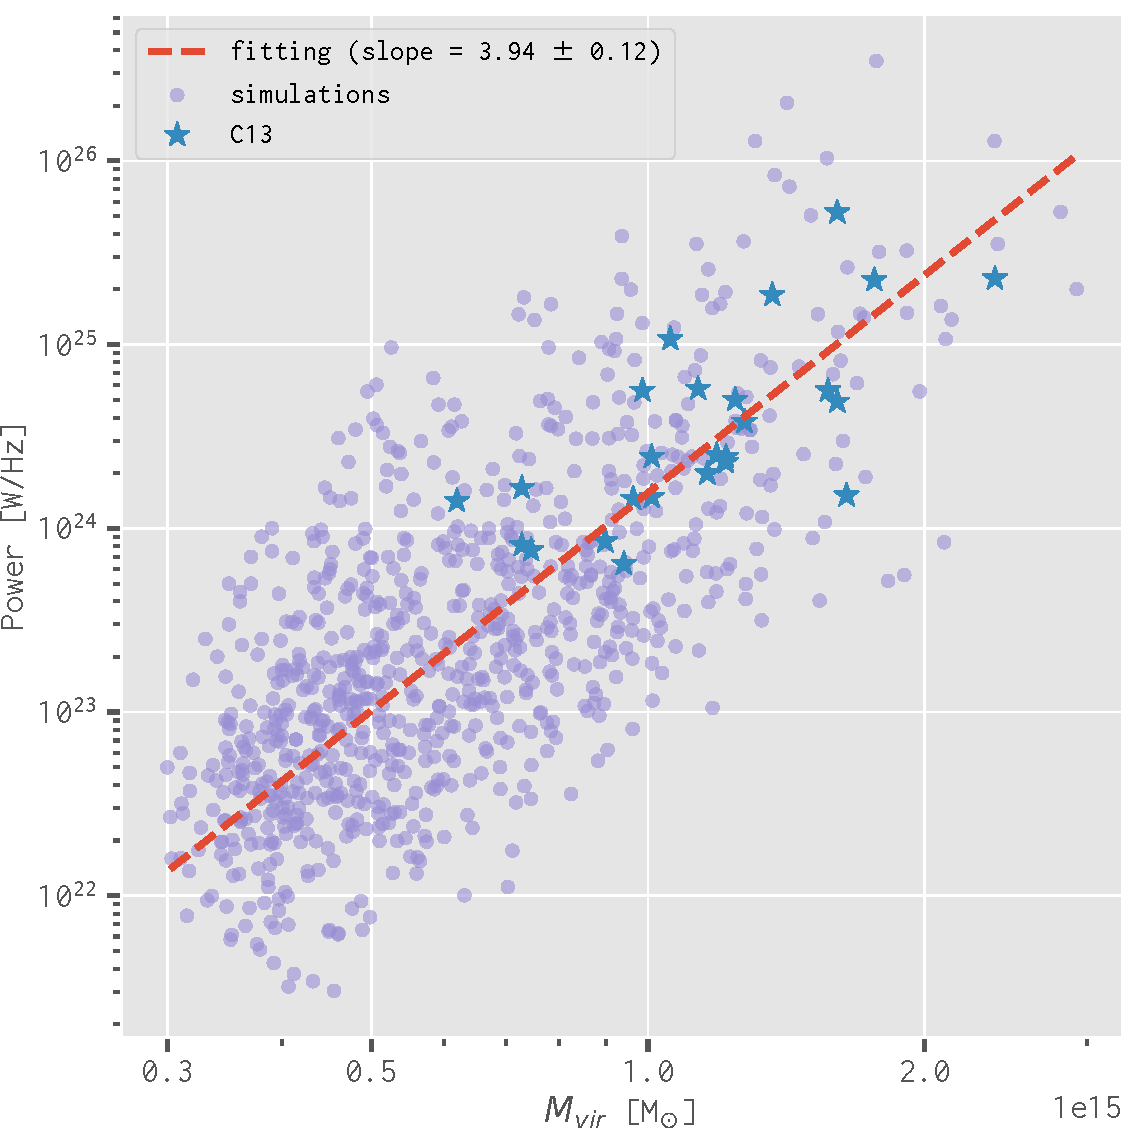
\includegraphics[width=\columnwidth]{halo-power-mvir}
      \caption{$P_{1400}$--$M_{\R{vir}}$ 标度关系的对比}
    \end{figure}

    \column{0.55\textwidth}
    \begin{figure}
      \centering
      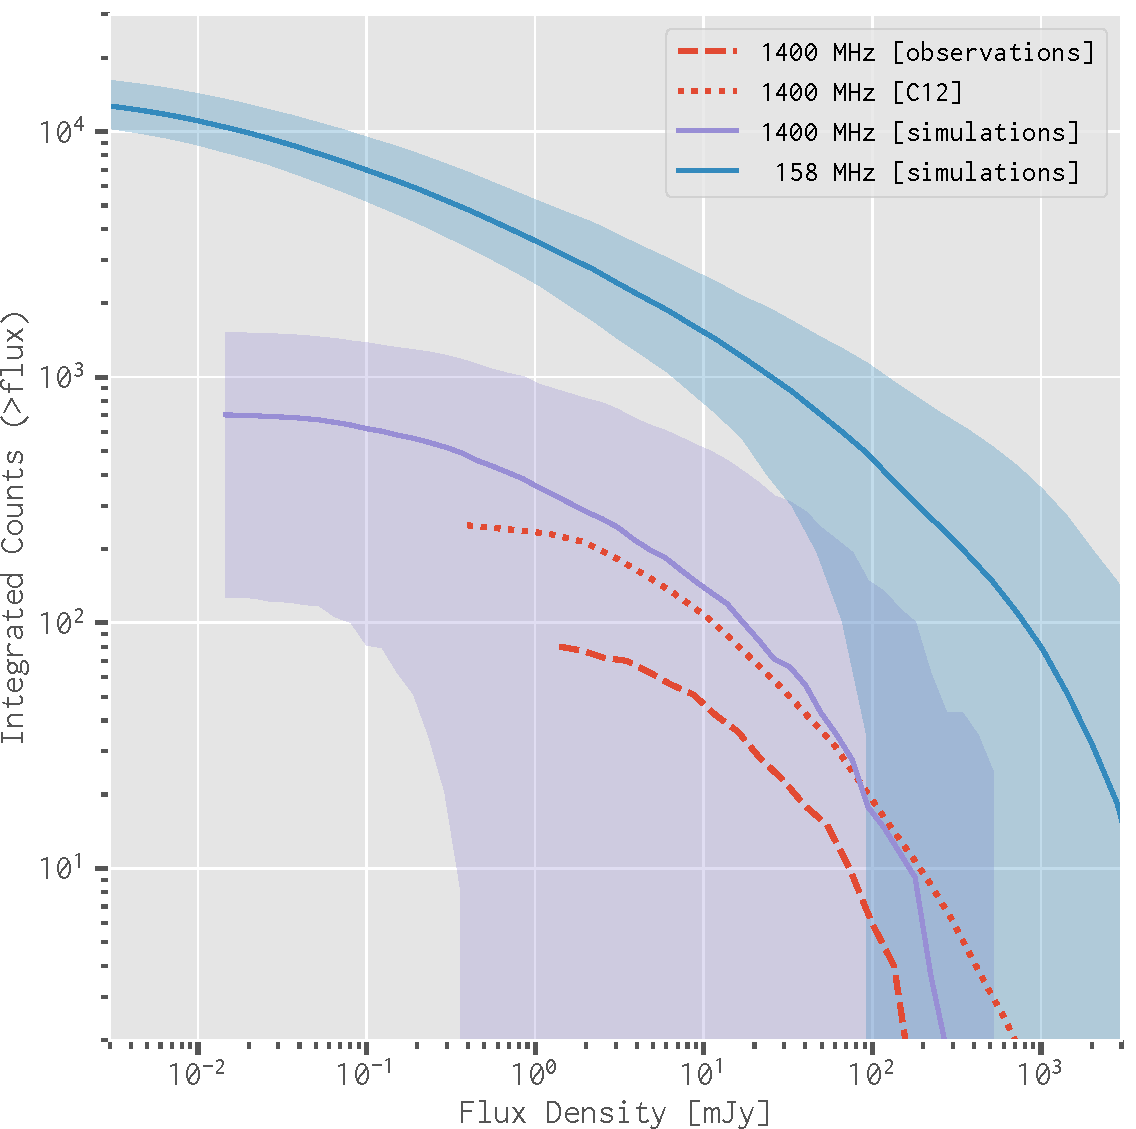
\includegraphics[width=\columnwidth]{fluxfunc-simucomp}
      \caption{\SI{1.4}{\GHz} 流量函数的对比}
    \end{figure}
  \end{columns}
\end{frame}

%............
\begin{frame}[subsec]
  \frametitle{射电晕天图生成}
  \begin{itemize}
    \item 射电晕在频率 $\nu$ 处的功率和流量密度:
      \begin{align}
        P_{\R{halo}}(\nu)
          & = \frac{4\Cpi}{3} r^3_{\R{halo}} J_{\R{syn}}(\nu) , \\
        S_{\R{halo}}(\nu)
          & = \frac{(1+z_{\R{sim}}) P_{\R{halo}}[\nu (1+z_{\R{sim}})]}{
            4\Cpi D^2_{\!L}(z_{\R{sim}})} ,
      \end{align}
      $D_{\!L}$ 是光度距离,因子 $(1+z_{\R{sim}})$ 为 $K$ 修正
    \item 射电晕的角向平均亮度分布:
      \begin{equation}
        I_{\nu}(\theta) = I_{\nu,0} \exp
          \left( -\frac{3\theta}{\theta_{\R{halo}}} \right) ,
      \end{equation}
      $\theta = r / D_{\!A}(z_{\R{sim}})$ 为角半径,
      $I_{\nu,0}$ 为中心亮度
    \item 利用 Rayleigh--Jeans 近似,表示为亮温度分布
  \end{itemize}
\end{frame}

%---------------------------------------------------------------------
\subsection{其他前景成分}

%............
\begin{frame}[subsec]
  \frametitle{银河系同步辐射}
  \begin{itemize}
    \item 以 Haslam \SI{408}{\MHz} 全天图为模板,
      按幂律形式向低频外延:
      \begin{equation}
        T_b^{\R{syn}}(\hat{\B{r}}, \nu)
          = T_b^{\R{haslam}}(\hat{\B{r}})
            \left( \frac{\nu}{\SI{408}{\MHz}}
            \right)^{-\alpha_{\R{syn}}(\hat{\B{r}})}
      \end{equation}
    \item $T_b^{\R{haslam}}(\hat{\B{r}})$
      为银河系 $\hat{\B{r}}$ 处的 \SI{408}{\MHz} 亮温度;\\
      使用 \cite{remazeilles2015} 重新处理的全天图
    \item $\alpha_{\R{syn}}(\hat{\B{r}})$ 为同步辐射谱指数;\\
      使用 \cite{giardino2002} 提供的谱指数全天分布图
  \end{itemize}
\end{frame}

%............
\begin{frame}[subsec]
  \frametitle{银河系自由—自由辐射}
  \begin{itemize}
    \item 自由–自由辐射和 Hα 辐射联系紧密
    \item Hα 辐射易被尘埃吸收,需要修正:
      \begin{equation}
        I_{\R{Hα}}^{\R{corr}}(\hat{\B{r}})
          = I_{\R{Hα}}(\hat{\B{r}}) \times
            10^{0.0185 \, f_d \, D(\hat{\B{r}})} ,
      \end{equation}
      $D(\hat{\B{r}})$ 是尘埃柱密度分布图,\\
      $f_d$ 是尘埃在视线方向上的有效吸收比例
    \item 在频率 $\nu$ 处的自由—自由辐射:
      \begin{equation}
        T_b^{\R{ff}}(\hat{\B{r}}, \nu)
          = 38.86 \,\nu^{-2.1} 10^{(290/T_e)} \, T_e^{0.667} \,a(\nu, T_e)
            \left[ \frac{I_{\R{Hα}}^{\R{corr}}(\hat{\B{r}})}{\si{\rayleigh}}
            \right] \quad [\si{\kelvin}]
      \end{equation}
    \item $a(\nu, T_e)$ 是光深的修正因子:
      \begin{equation}
        a(\nu, T_e) =
          0.183 \,\nu^{0.1} T_e^{-0.15}
          \left[ 3.91 - \ln \nu + 1.5 \ln T_e \right]
      \end{equation}
    \item 本文取 $f_d = 0.33$ 和 $T_e = \SI{7000}{\kelvin}$
  \end{itemize}
\end{frame}

%............
\begin{frame}[subsec]
  \frametitle{河外点源}
  \begin{itemize}
    \item 继承自我们之前的一项工作:\cite{wang2010}
    \item 模拟了下述 4 类点源:
      \begin{enumerate}
        \item FR I 型和 II 型射电星系
        \item 恒星形成星系
        \item 射电宁静 AGN
        \item GHz 倒转谱和致密陡谱 AGN
      \end{enumerate}
    \item 第 1--3 类点源的模拟使用了 \cite{wilman2008} 针对 SKA 的模拟结果
    \item 第 4 类点源的模拟使用了相应的光度函数和频谱模型
  \end{itemize}
\end{frame}

%---------------------------------------------------------------------
\subsection{频率维度的加窗处理}

%............
\begin{frame}[subsec]
  \frametitle{频率维度的加窗处理}
  \myfigure{%
    width=\textwidth,
  }{ft-sidelobes}{%
    使用 Blackman--Nuttall 窗函数与否的 Fourier 变换结果对比;\\
    输入信号为 $y = (x / 158)^{-2}$.
  }
\end{frame}

%---------------------------------------------------------------------
\subsection{SKA1-Low 阵列布局}

%............
\begin{frame}[subsec]
  \frametitle{SKA1-Low~阵列布局}
  \begin{columns}
    \column{0.55\textwidth}
    \myfigure{%
      width=\columnwidth,
    }{SKA1low-config-central}{%
      中央区域 ($R \le \SI{1700}{\meter}$) 的站点布局:
      核心区域 ($R \le \SI{500}{\meter}$) 224 个,
      以及 12 个站点团
    }

    \column{0.55\textwidth}
    \myfigure{%
      width=\columnwidth,
    }{SKA1low-config-outside}{%
      外围区域的 36 个站点团\\(\cite{dewdney2016ska})
    }
  \end{columns}
\end{frame}

%---------------------------------------------------------------------
\subsection{参考文献}

\begin{frame}[allowframebreaks]{参考文献}
  \printbibliography[heading=none]
\end{frame}

\end{document}
